\documentclass[conference]{IEEEtran}
\IEEEoverridecommandlockouts


%\usepackage{tikz}
\usepackage{amsmath}
\usepackage{multirow}
\usepackage{makecell}
\usepackage{verbatim}
\usepackage{subfig}
\usepackage{url}

%\usepackage{markdown}

%\usepackage{cite} % will generate Runaway argument? error, we also need to replace '#' with. '##' in the bib file for all URL
\usepackage{ulem}
\usepackage{pifont}

%\usepackage[notextcomp]{stix}
\usepackage{graphicx}
\usepackage{color, colortbl}


\usepackage{listings}
%\usetikzlibrary{positioning,shadows.blur,fit}
\definecolor{auburn}{rgb}{0.43, 0.21, 0.1}
\definecolor{codegreen}{rgb}{0,0.6,0}
\definecolor{codegray}{rgb}{0.5,0.5,0.5}
\definecolor{codepurple}{rgb}{0.58,0,0.82}
\lstdefinelanguage
   [x64]{Assembler}     % add a "x64" dialect of Assembler
   [x86masm]{Assembler} % based on the "x86masm" dialect
   % with these extra keywords:
   {morekeywords={CDQE,CQO,CMPSQ,CMPXCHG16B,JRCXZ,LODSQ,MOVSXD,movl,addl,subl, %
                  pushq,popq,leaq,cmpq,POPFQ,PUSHFQ,SCASQ,STOSQ,IRETQ,RDTSCP,SWAPGS, %
                  rax,rdx,rcx,rbx,rsi,rdi,rsp,rbp,retq,callq,movq, %
                  r8,r8d,r8w,r8b,r9,r9d,r9w,r9b,r10,r11,r12,r15,enclu,mfence,lfence,cmova,cmovg,cmovl}} % etc.
\lstdefinestyle{mystyle}{
    backgroundcolor=\color{white},   
    commentstyle=\color{blue},
    keywordstyle=\color{auburn},
    numberstyle=\tiny\color{codegray},
    stringstyle=\color{codepurple},
    basicstyle=\footnotesize,
    breakatwhitespace=false,         
    breaklines=true,                 
    captionpos=b,                    
    keepspaces=true,                 
    numbers=left,                    
    numbersep=5pt,                  
    showspaces=false,                
    showstringspaces=false,
    showtabs=false,                  
    tabsize=2
}
\lstset{
  language=[x64]Assembler,
  style=mystyle
}

% for IEEE format
% \usepackage{appendix}
\usepackage{cite}


\usepackage{amsmath,amssymb,amsfonts}
\usepackage{algorithmic}
\usepackage{textcomp}
\usepackage{xcolor}
\def\BibTeX{{\rm B\kern-.05em{\sc i\kern-.025em b}\kern-.08em
    T\kern-.1667em\lower.7ex\hbox{E}\kern-.125emX}}
    

\newcommand\xiaofeng[1]{\textcolor{red}{\{\textbf{xiaofeng:} {\em#1}\}}}
\newcommand{\ignore}[1]{}
\newcommand\todo[1]{\textcolor{blue}{\{\textbf{To-Do:} {\em#1}\}}}

\newcommand\wenhao[1]{\textcolor{magenta}{\{\textbf{wenhao:} {\em#1}\}}}
\newcommand\hongbo[1]{\textcolor{teal}{\{\textbf{hongbo:} {\em#1}\}}}
\newcommand\weijie[1]{\textcolor{brown}{\{\textbf{weijie:} {\em#1}\}}}
\newcommand\yaosong[1]{\textcolor{gray}{\{\textbf{yaosong:} {\em#1}\}}}
\newcommand\xinyu[1]{\textcolor{cyan}{\{\textbf{xinyu:} {\em#1}\}}}
\newcommand\kai[1]{\textcolor{blue}{\{\textbf{kai:} {\em#1}\}}}

% for revision
%\newcommand\revise[1]{{\color{red}{#1}}}
\newcommand\revise[1]{{#1}}

\pagestyle{plain}


%last page balance
\usepackage{flushend}


\begin{document}

\title{Practical and Efficient in-Enclave Verification of Privacy Compliance}


%\title{Confidential Attestation: Practical and Efficient in-Enclave Verification of Privacy Compliance}
%\title{Confidential Attestation: Efficient in-Enclave Verification of Privacy Policy Compliance}

%\title{Privacy-preserving TEE on a service-oriented environment

\author{\IEEEauthorblockN{1\textsuperscript{st} Given Name Surname}
\IEEEauthorblockA{\textit{dept. name of organization (of Aff.)} \\
\textit{name of organization (of Aff.)}\\
City, Country \\
email address}
\and
\IEEEauthorblockN{2\textsuperscript{nd} Given Name Surname}
\IEEEauthorblockA{\textit{dept. name of organization (of Aff.)} \\
\textit{name of organization (of Aff.)}\\
City, Country \\
email address}
\and
\IEEEauthorblockN{3\textsuperscript{rd} Given Name Surname}
\IEEEauthorblockA{\textit{dept. name of organization (of Aff.)} \\
\textit{name of organization (of Aff.)}\\
City, Country \\
email address}
\and
\IEEEauthorblockN{4\textsuperscript{th} Given Name Surname}
\IEEEauthorblockA{\textit{dept. name of organization (of Aff.)} \\
\textit{name of organization (of Aff.)}\\
City, Country \\
email address}
\and
\IEEEauthorblockN{5\textsuperscript{th} Given Name Surname}
\IEEEauthorblockA{\textit{dept. name of organization (of Aff.)} \\
\textit{name of organization (of Aff.)}\\
City, Country \\
email address}
\and
\IEEEauthorblockN{6\textsuperscript{th} Given Name Surname}
\IEEEauthorblockA{\textit{dept. name of organization (of Aff.)} \\
\textit{name of organization (of Aff.)}\\
City, Country \\
email address}
}
% \author{}


%\keywords{Intel SGX, PCC, Confidentiality, Verification}

\maketitle
%corresponding authors
\begingroup\renewcommand\thefootnote{\textsection}
\footnotetext{Corresponding authors}
\endgroup

\begin{abstract}

A trusted execution environment (TEE) such as Intel Software Guard Extension (SGX) runs attestation to prove to a data owner the integrity of the initial state of an enclave, including the program to operate on her data. For this purpose, the data-processing program is supposed to be open to the owner or a trusted third party, so its functionality can be evaluated before trust being established. In the real world, however, increasingly there are application scenarios in which the program itself needs to be protected (e.g., proprietary algorithm). So its compliance with privacy policies as expected by the data owner should be verified without exposing its code. 


To this end, this paper presents \textsc{Deflection}, a new model for TEE-based \revise{delegated and flexible in-enclave code verification}. Given that the conventional solutions do not work well under the resource-limited and TCB-frugal TEE, we come up with a new design inspired by Proof-Carrying Code\DIFdelbegin \DIFdel{that allows an untrusted out-enclave generator to analyze and instrument the source code of a program when compiling it into binary and a trusted in-enclave consumer efficiently verifies the correctness of the instrumentation and the presence of other protection before running the binary.
}\DIFdelend \DIFaddbegin \DIFadd{.
%DIF >  that allows an untrusted out-enclave generator to analyze and instrument the source code of a program when compiling it into binary and a trusted in-enclave consumer efficiently verifies the correctness of the instrumentation and the presence of other protection before running the binary. 
}\DIFaddend Our design strategically moves most of the workload to the code generator, which is responsible for producing easy-to-check code, while keeping the consumer simple. Also, the whole consumer can be made public and verified through a conventional attestation. We implemented this model on Intel SGX and demonstrate that it introduces a very small part of TCB. We also thoroughly evaluated its performance on micro- and macro- benchmarks and real-world applications, showing that the design only incurs a small overhead when enforcing several categories of security policies.



%technology using Intel SGX for multiple scenarios. CAT is designed with a Proof-Carrying Code (PCC) concept composed of an LLVM-based code producer and Intel SGX-based code consumer. We implement CAT and thoroughly evaluate it on real SGX hardware. It can effectively prevent data breaches and preserve code confidentiality at the same time. Moreover, the TCB of our design is smaller than mostly related approaches. Performance evaluation shows low overhead (about 18\% on average) in running common micro-benchmarks and acceptable overhead (less than 23\% on average) in running more realistic workloads.
%Security analysis elaborates that attackers only have very limited ways to leakage data and

\end{abstract}

% for Oakland
%\begin{IEEEkeywords}
%Intel SGX, PCC, Confidentiality, Verification
%\end{IEEEkeywords}
\DIFaddbegin 

\begin{IEEEkeywords}
\DIFadd{Intel SGX, Confidential Computing, Proof-Carrying Code, Enclave Shielding Runtime
}\end{IEEEkeywords}
\DIFaddend 


%Intel Software Guard Extension (SGX) has been studied widely for protecting data and code under many circumstances, especially on cloud computing platforms. Data owners always want their data to be used in a highly secure way, so SGX is naturally a practical and effective way that can be leveraged in such scenarios. Intel SGX provides a relatively trustworthy execution environment for preventing data from being observed by the outside world. This crucial step requires remote attestation protocols, and meanwhile, the service provider's code needs to be exposed. However, service providers may not want their data-processing code to be public.

%To address the dilemma, this paper presents CAT, a new practical confidential attestation technology using Intel SGX for multiple scenarios. CAT is designed with a Proof-Carrying Code (PCC) concept composed of an LLVM-based code producer and Intel SGX-based code consumer. We implement CAT and thoroughly evaluate it on real SGX hardware. It can effectively prevent data breaches and preserve code confidentiality at the same time. Moreover, the TCB of our design is smaller than mostly related approaches. Performance evaluation shows low overhead (about 18\% on average) in running common micro-benchmarks and acceptable overhead (less than 23\% on average) in running more realistic workloads.

\section{Introduction}\label{sec-introduction}

Recent years have witnessed the emergence of hardware trusted execution environments (TEEs) that enable efficient computation on untrusted platforms. 
%A prominent example is Intel SGX~\cite{mckeen2013innovative}, a TEE widely deployed on commercial-off-the-shelf (COTS) desktops and server processors, providing secure memory called \textit{enclave} to host confidential computing on sensitive data, which are protected from the adversary in control of the operating system and even with physical access to the data-processing machine. 
A prominent example such as Intel SGX~\cite{mckeen2013innovative} has already been supported by major cloud providers today, including Microsoft Azure and Google Cloud~\cite{russinovich2017introducing,asylo2019}, and its further adoption has been facilitated by the Confidential Computing Consortium~\cite{ccc2019}, a Linux Foundation project that brings together the biggest technical companies such as Intel, Google, Microsoft and IBM etc. However, before TEEs can see truly wide deployment for real-world confidential computing, key technical barriers still need to be overcome, \textit{remote attestation} in particular.

\vspace{3pt}\noindent\textbf{Remote attestation}. At the center of a TEE's trust model is remote attestation (RA), which allows the user of confidential computing to verify that the enclave code processing her sensitive data is correctly built and operates on a genuine TEE platform~\cite{zhang2017presence}, so her data is well protected. This is done on SGX through establishing a chain of trust rooted at a platform attestation key 
which is used to generate a \textit{Quote} -- a signed report that contains the measurement of the code and data in an enclave; the Quote is delivered to the data owner and checked against the signature and the expected measurement hash. This trust building process is contingent upon the availability of the measurement, which is calculated from the enclave program either by the data owner when the program is publicly available or by a trusted third party working on the owner's behalf. This becomes problematic when the program itself is private and cannot be exposed.
Programs may have exploitable bugs or they may write information out of the enclave through corrupted pointers easily.

For example, a  pharmaceutical company can run its proprietary algorithm inside an enclave hosting patient medical records, without exposing the algorithm but can still ensure the hospital (the data owner) the compliance of its data use with the hospital's privacy policy. Another example can be a privacy-preserving credit evaluation service, in which a customer's transactions are only exposed to an enclave running the credit evaluation code in compliance with a set of public privacy-protection rules (such as GDPR).
We consider confidential computing as a service (\textit{CCaaS}) as a privacy extension of today's online data processing services like machine-learning as a service~\cite{russinovich2017introducing}. CCaaS is hosted by the party that operates its own target binary on the data provided by its owner (e.g., an online image classifier to label uploaded user photos). With applications of this kind on the rise, new techniques for protecting both data and code privacy are in great demand.  

\vspace{3pt}\noindent\textbf{Challenges}. To address this problem, we present in this paper a novel \textit{Delegated and flexible in-enclave code verification} (\textsc{Deflection}) model to enable verification of an enclave program's compliance with user-defined security policies without exposing its source or binary code to unauthorized parties involved. Under the \textsc{Deflection} model, a \textit{bootstrap enclave} whose code is public and verifiable through the Intel's remote attestation, is responsible for performing the compliance check on behalf of the participating parties, who even without access to the code or data to be attested, can be convinced that desired policies are faithfully enforced.  
However, building a system to support this model turns out to be nontrivial, due to the complexity in static analysis of enclave binary for policy compliance, the need to keep the verification mechanism, which is inside the enclave's \textit{trusted computing base} (\textit{TCB}), small, the demand for a quick turnaround from the enclave user, and the limited computing resources today's SGX provides (about 93 MB physical memory on most commercial hardware~\cite{chakrabarti2019scaling}). 
%Simply sand-boxing the enclave code to enforce security policies, however, does not work well. 
Although the shielding runtimes such as Library OSes~\cite{priebe2019sgx,shen2020occlum},  SCONE container~\cite{arnautov2016scone}, Ryoan sandbox~\cite{hunt2018ryoan} and the interpreters/compilers built for SGX~\cite{wang2019towards,wang2019running} enable confinement of unmodified binary in SGX  enclaves, they all rely on a heavy interface layer for in-enclave service code to interact with the OS/Hypervisor~\cite{lazard2018teeshift}, which introduces performance overhead. More importantly, the confinement mechanisms (sometimes including a whole interpreter) significantly increase the TCB, leading to a challenge in ensuring its security~\cite{van2019tale}. In our research, we studied popular shielding runtimes, Graphene-SGX even includes more than 100 kLoCs, more than 50 MB in binary, based upon analysis of its code.

%\revise{\vspace{3pt}\noindent\textbf{Existing architectures of shielding runtimes}.  Library OSes~\cite{priebe2019sgx,shen2020occlum},  containers~\cite{arnautov2016scone}, and sandboxes~\cite{hunt2018ryoan} support  running  unmodified binary  in  SGX  enclaves. These solutions rely on a heavy interface layer for in-enclave service code interacting with the OS/Hypervisor, with a non-negligible performance overhead.Interpreters and compilers built for SGX~\cite{wang2019towards,wang2019running} also support in-enclave secure computing. However, they either introduce the language runtime environment or the whole code generator into the TCB, leading to a big uncertainty to security and performance~\cite{van2019tale}. }

%\weijie{Highlight the design principle of \textit{separating mechanism and policy}}

A promising direction we envision that could lead to a practical solution is \textit{proof-carrying code} (\textit{PCC})~\cite{necula1997proof,schneider2001language}, a technique that enables a \textit{verification condition generator} (\textit{VCGen})~\cite{colby2000certifying,leroy2006formal,pirzadeh2010extended} to analyze a program and create a proof that attests the program's adherence to policies, and a \textit{proof checker} to verify the proof and the code. The hope is to keep the VCGen outside the enclave while keeping the proof checker inside the enclave small and efficient.  The problem is that this \textit{cannot} be achieved by existing approaches, which utilize formal verification (such as~\cite{necula2001oracle,pirzadeh2010extended}) to produce a proof that could be considerably larger than the original code. Actually, today's formal verification techniques, theorem proving in particular, are still less scalable, difficult to handle large code blocks when constructing a security proof~\cite{sinha2015moat}. 


\vspace{3pt}\noindent\textbf{Our solution}. In our research, we developed a new technique to instantiate the \textsc{Deflection} model on SGX. Our approach, has been inspired by PCC, but relies on program analysis and Software-based Fault Isolation (SFI) techniques, particularly out-of-enclave targeted instrumentation for lightweight in-enclave information-flow confinement, instead of heavyweight theorem proving to ensure policy compliance of enclave code. More specifically, \textsc{Deflection} operates an untrusted \textit{code producer} as a compiler to build the binary code for a data-processing program (called \textit{target program}) and instrument it with a set of \textit{security annotations} for enforcing desired policies at runtime, together with a lightweight trusted \textit{code consumer} running in the bootstrap enclave to statically verify whether the target code indeed carries properly implanted security annotations.


To reduce the TCB and in-enclave computation, \textsc{Deflection} is designed to simplify the verification step by pushing out most computing burden to the code producer running outside the enclave. More specifically, the target binary is expected to be well formatted by the producer, with all its indirect control flows resolved, all possible jump target addresses specified on a list and enforced by security annotations.  In this way, the code consumer can check the target binary's policy compliance through lightweight \textit{Recursive Descent Disassembly} to inspect its complete control flow (Section~\ref{subsec-boundarychecking}), so as to ensure the presence of correctly constructed security annotations in front of each critical operation, such as load, store, enclave operations like OCall, and stack management (through a shadow stack). Any failure in such an inspection causes the rejection of the program. Also, since most code instrumentation (for injecting security annotations) is tasked to the producer, the code consumer does not need to make any change to the binary except relocating it inside the enclave. As a result, we only need a verifier with a vastly simplified disassembler, instead of a full-fledged, complicated binary analysis toolkit, to support categories of security policies, including data leak control, control-transfer management, self-modifying code block and side/covert channel mitigation in a small-size machine-language format (Section~\ref{subsec-policies}); in further work, other proofs could be extended given a formal model of the x64 instruction set (e.g., as in~\cite{morrisett1999system}).
A wider spectrum of policies can also be upheld by an extension of \textsc{Deflection}, as discussed in the paper (Section~\ref{sec-discussion}). 

%and multi-user isolation 

%To reduce the TCB and computations inside the bootstrap enclave, we move as much annotation generation workload as possible to the code producer and design simple-to-verify annotation formats. In this way, the code consumer only includes a simple disassembler, instead of a full-fledged, complicated binary analysis component, to verify the security checks. The verifier performs only a few simple binary rewriting by overwriting immediate operands in instructions and the policy-compliance verification is performed by traversing the code in a recursive descent manner. \kai{Reaching here, readers may think the contribution is only to shrink the code, and move unnecessary code outside the verifier.} The verifier defers the challenging problem of resolving indirect control flow to the code producer, requiring the code producer to provide a list of indirect control flow targets and security annotation before each indirect control flow for verifying the actual target at run-time. 


We implemented \textsc{Deflection} in our research, building the code producer on top of the LLVM compiler infrastructure and the code consumer based upon the Capstone disassembly framework~\cite{capstone} and the core disassembling engine for x86 architecture. 
Using this unbalanced design, our in-enclave program has only 2000 lines of source code, which is significantly smaller than other shielding runtimes. 
To port theorem prover Z3 into SGX, with 26 MB used in Moat~\cite{sinha2015moat}, is not easy as well, not only because of its size but also its inability to be statically linked against an enclave.
We further evaluated our implementation on micro-benchmarks (nBench), as well as macro-benchmarks, including credit scoring, HTTPS server, and also basic biomedical analysis algorithms.
%(sequence alignment, sequence generation, etc.) under the scenario of Confidential Computing as a Service. 

%For example, Ryoan uses NaCl's core library, whose binary is around 20 MB \weijie{Ryoan's code is released} and the LibOSes used by Graphene-SGX and Occlum are even bigger.
%PANOPLY offers two orders of magnitude lower TCB(about 20 KLOC in total
%libz3.so is 26M

\textsc{Deflection} incurs on average (calculated by geometric mean) 20\% performance overhead
%and less than 30\% storage overhead 
enforcing all the proposed security policies, and leads to around 10\% performance overhead
%and less than 20\% storage overhead 
without side/covert channel mitigation.
We have released our code on Github~\cite{our-prototype}.

%We observed a memory overhead from 3.8\% and 134\% and a slowdown merely 1.003$\times$ to 1.548$\times$. 
%\wenhao{geometry mean of the overhead is better}  

%on simple application bench
%geometry mean of performance overhead of P1~P5: 1.098
%geometry mean of performance overhead of P1~P6: 1.193
%geometry mean of storage overhead of P1~P5: 1.181
%geometry mean of storage overhead of P1~P6: 1.295
%on nbench
%geometry mean of performance overhead of P1~P5: 1.111
%geometry mean of performance overhead of P1~P6: 1.176

%The size of the code consumer is only 7.7 MB in total\kai{users may not know how small is 7.7MB, you may compare with other disassembing engines}\weijie{comparing ours with the verification toolset used by MOAT (disassembling and instruction modeling using BAP + transformation and annotation generation using BoogiePL + theorem proving using Z3), comparing ours with Ryoan (sandbox using NaCl)}, way less than a compiler/interpreter or a sandbox. The evaluation on several benchmarks and genomic processing algorithms shows that the size of the additional security annotation is between 3.8\% and 134\%, while the running time overhead is between 0.3\% and 54.8\%.


%the untrusted code producer by retrofitting the LLVM compiler infrastructure with a IR-level pass and a customized back-end pass. The code consumer is implemented inside the bootstrap enclave by tailoring the Capstone disassembly framework~\cite{capstone} and retaining the core disassembling engine for x86 architecture. The size of the code consumer is only 7.7 MB in total\kai{users may not know how small is 7.7MB, you may compare with other disassembing engines}\weijie{comparing ours with the verification toolset used by MOAT (disassembling and instruction modeling using BAP + transformation and annotation generation using BoogiePL + theorem proving using Z3), comparing ours with Ryoan (sandbox using NaCl)}, way less than a compiler/interpreter or a sandbox. The evaluation on several benchmarks and genomic processing algorithms shows that the size of the additional security annotation is between 3.8\% and 134\%, while the running time overhead is between 0.3\% and 54.8\%.

\vspace{3pt}\noindent\textbf{Contributions}. The contributions are outlined as follows:

\vspace{3pt}\noindent$\bullet$\textit{ New model}. We propose \textsc{Deflection}, a \revise{portable framework} that extends today's TEE to maintain the data owner's trust in protection of her enclave data, without exposing the code of the data-processing program. This is achieved through enforcing a set of security policies through a publicly verifiable bootstrap enclave. This new attestation model enables a wide spectrum of applications with great real-world demand in the confidential computing era. 
%that can enforce the privacy and security policies of both the code and data provided by untrusted parties, while preserving the confidentiality of them. We find that a number of application scenarios can be benefited from the proposed model.
    
\vspace{3pt}\noindent$\bullet$\textit{ New techniques}. We present the design for instantiating \textsc{Deflection} on SGX, following the idea of PCC. Our approach utilizes out-of-enclave code analysis and instrumentation to minimize the workload for in-enclave policy compliance check, which just involves a quick run of a well-formatted target binary for inspecting correct instrumentation. This simple design offers a much smaller TCB compared with existing solutions.   

%which consists of an untrusted code producer (which runs outside of the enclave) and a trusted code consumer (which runs in the bootstrap enclave). We illustrate how to use CAT to implement memory leak prevention policies and common SGX side/covert channel prevention policies. Such a design reduces the size of and computation inside the trusted code consumer and is scalable to real world applciations. 

\vspace{3pt}\noindent$\bullet$\textit{ Implementation and evaluation}. We implemented our design of \textsc{Deflection} and extensively evaluated our prototype on micro- and macro- benchmarks, together with popular biomedical algorithms.  Our experiments show that \textsc{Deflection} effectively enforces various security policies at small cost, with \revise{multiple level protections}. 


%\footnote{The current project code is available on (github link).}
%\end{itemize}

%\vspace{3pt}\noindent\textbf{Roadmap}. The rest of this paper is organized as follows. Section~\ref{sec-background} provides background information on Intel SGX and PCC; Section~\ref{sec-CAT} elaborates the Confidential attestation \weijie{} model, our design goals and the threat model; Section~\ref{sec-design} and Section~\ref{sec-implementation} provide the detailed design and implementation of our system;
% \textit{CAT}, and our system implementation in deploying PCC for the SGX environment. Section~\ref{sec-evaluation} reports the evaluation of our implementation; 
%discusses impacts of attacks against our system and performance evaluation. Discussions are made in Section~\ref{sec-discussion}. Section~\ref{sec-relatedwork} compares our work with related prior research, and Section~\ref{sec-conclusion} concludes the paper.

\section{Background}\label{sec-background}

\noindent\textbf{Intel SGX}. Intel SGX~\cite{mckeen2013innovative} is a user-space TEE, which is characterized by flexible process-level isolation. Such protection, however, comes with in-enclave resource constraints. Particularly, only 128 MB (256 MB for some new processors) encryption protected memory is reserved. Although virtual memory support is available, it incurs significant overheads in paging~\cite{arnautov2016scone}. 


 %In fact, due to the memory encryption engine carved from the EPC memory and the lingering of SGX SDK, there is around 90 MB physical memory that could be allocated for user programs.
Another problem caused by SGX's design is a large attack surface. The application can invoke a pre-defined function inside the enclave, passing input parameters and pointers to shared memory within the application. Those invocations from the application to the enclave are called ECall. When an enclave executes, it can perform an OCall to a pre-defined function in the application. Contrary to an ECall, an OCall cannot share enclave memory with the application, so it must copy the parameters into the application memory before the OCall. When an enclave program contains memory vulnerabilities, attacks can happen to compromise enclave's privacy protection. Prior research demonstrates that a Return-oriented programming (ROP) attack can succeed in injecting malicious code inside an enclave, which can be launched by the OS, Hypervisor, or BIOS~\cite{lee2017hacking,biondo2018guard,schwarz2019practical}. %Deploying the Control flow integrity (CFI) in the enclave also needs to consider the SGX-specific features~\cite{lee2017hacking}.
Another security risk is side-channel leak~\cite{schwarz2017malware,lee2017inferring,gras2018translation}, caused by the thin software stack inside an enclave (for reducing TCB),  which often has to resort to the OS for resource management (e.g., paging, I/O control). Particularly, an OS-level adversary can perform a controlled side channel attack (e.g.,~\cite{xu2015controlled}).
%Also in the threat model is the physical adversary, such as a system administrator, who tries to gain unauthorized access to a TEE’s computing units to compromise its integrity or confidentiality.

%\weijie{remove this paragraph}
%\vspace{3pt}\noindent\textbf{SGX remote attestation}. As mentioned earlier, attestation allows a remote user to verify that the enclave is correctly constructed and run on a genuine SGX-enabled platform. In Intel’s attestation model, three parties are involved: (1) the Independent Software Vendor (ISV) who is registered to Intel as the enclave developer; (2) the Intel Attestation Service (IAS) hosted by Intel to help enclave verification,
%\footnote{SGX now supports both the Intel Enhanced Privacy ID (Intel EPID) based Intel Attestation Service (IAS) and the Elliptic Curve Digital Signature Algorithm (ECDSA) based third-party attestation with Intel SGX Data Center Attestation Primitives (Intel SGX DCAP) to generate and verify the quote. The signing and verifying algorithms are orthogonal to the main part of the paper.}
%and for simplicity we assume the IAS based attestation is used.}
%and (3) the SGX-enabled platform that operates SGX enclaves. The attestation begins with the ISV sending an attestation request challenge, which can be generated by an enclave user or a data owner who wants to perform the attestation with the enclave to check its state. Upon recipient of the challenge, the enclave then generates a verification report including the enclave measurement, which can be verified by a quoting enclave (QE) through \textit{local attestation}. The QE signs the report using the attestation key and the generated \textit{quote} is forwarded to the Intel Attestation Service (IAS). 
%The IAS then checks the quote and signs the verification result using Intel's private key. The ISV can then validate the attestation result based upon the signature and the enclave measurement.

%\weijie{shrink and rewrite the following subsection}

\vspace{3pt}\noindent\textbf{PCC}. PCC is a mechanism that allows a host system to verify an application's properties with a proof accompanying the application's executable code.
Traditional PCC schemes tend to utilize formal verification for proof generation and validation. Techniques for this purpose includes verification condition generation~\cite{homeier1995mechanically,colby2000certifying}, theorem proving~\cite{paulson2000isabelle,de2008z3,bertot2013interactive}, and proof checking~\cite{appel2003trustworthy}, which typically work on type-safe intermediate languages (IL) or higher level languages. A problem here is that up to our knowledge, no formal tool today can automatically transform a binary to IL for in-enclave verification. BAP~\cite{brumley2011bap} disassembles binaries and lifts x86 instructions to a formal format, but it does not have a runtime C/C++ library for static linking, as required for an enclave program.
Moreover, the PCC architecture relies on the correctness of the VCGen and the proof checker, so a direct application of PCC to confidential computing needs to include both in TCB. This is problematic due to their complicated designs and implementations, which are known to be error-prone~\cite{necula2001oracle}. Particularly, today's VCGens are built on either an interpreter/compiler even a virtual machine~\cite{leroy2006formal}, and therefore will lead to a huge TCB. Prior attempts~\cite{appel2001foundational} to move VCGen out of TCB are found to have serious performance impacts, due to the significantly increased proof size growing exponentially with the size of the program that needs to be certified~\cite{necula1997proof}. \ignore{ It is common to have a proof 1000 times larger than the code~\cite{pirzadeh2010extended}. The proof/certificate in PCC is a formal representation that can be encoded as e.g. LF term. Such proof terms include a lot of repetition which means it includes huge certificates. } Although techniques are there to reduce the proof size~\cite{appel2001foundational,pirzadeh2010extended},\ignore{ e.g. OPCC introduces a non-deterministic proof checker that makes the proof 30 times smaller. However, } they are too complicated to scale to real-world applications~\cite{appel2003trustworthy}. 
%Therefore as far as we are aware, no existing PCC techniques can be directly applied to enable the CAT model on today's TEE. 

\section{Deflection}\label{sec-CAT}
%\vspace{3pt}\noindent\textbf{Motivating Example}.

%\subsection{Motivating Example}\label{subsec-motivation}

\DIFaddbegin \DIFadd{In this section, we present the }\textit{\DIFadd{DElegated and  FLexible  in-Enclave  Code verification}} \DIFadd{(}\textsc{\DIFadd{Deflection}}\DIFadd{) model to allow the data owner to verify that the enclave code satisfies predefined security policy requirements without undermining the privacy of the enclave code.
}

\DIFaddend Consider an organization that provides data-processing services, such as image editing, tax preparation, personal health analysis and deep learning inference as a service. To use the services, \DIFdelbegin \DIFdel{their }\DIFdelend customers need to upload their sensitive data, such as images, tax documents, and health data, to the hosts operated by the organization. To avoid exposing the data, the services run inside SGX enclaves and need to prove to the customers that they are accessing to attested service programs. However, the organization may not want to release \DIFdelbegin \DIFdel{the }\DIFdelend proprietary programs to protect its intellectual property. \DIFdelbegin \DIFdel{This problem cannot be addressed by today's TEE design.  
}%DIFDELCMD < 

%DIFDELCMD < %%%
\DIFdel{In this section, we present the }\textit{\DIFdel{DElegated and  FLexible  in-Enclave  Code verification}} %DIFAUXCMD
\DIFdel{(}\textsc{\DIFdel{Deflection}}%DIFAUXCMD
\DIFdel{) model to allow the data owner to verify that the enclave code satisfies predefined security policy requirements without undermining the privacy of the enclave code}\DIFdelend \DIFaddbegin \DIFadd{Here, DEFLECTION can enforce the data privacy on behalf of the data-processing services.
Besides, the framework of our system is highly flexible, which means assembling new policies into current design can be very straightforward. Different on-demand policies can be appended/withdrawn to serve various goals. For example, DEFLECTION can make the quick patch possible on software level, just like the way people coping with 1-day vulnerabilities - emergency quick fix}\DIFaddend . 

 


%We also provide application scenarios for the CAT model, its design goals . We will further list the design goals in designing a practical CAT model in the context of Intel SGX, as well as the threat model considered in the paper. 

%Aiming to complete a system that can flexibly verify whether the code leaks data on SGX platforms, we propose Confidential Attestation. This technology can be used in different situations.
%In particular, we will enumerate all technical challenges needed to be overcome during building such a system, and will elaborate the threat model during achieving all purposes of our design.

%The service provider often has secret algorithms or business logic that can not be exposed. As an entity that needs/should to compute a secret value, it may be willing to secure the private algorithm during delivery. Meanwhile, the service provider could sell the intelligent property to a user who wants to process the secret data for a trustworthy and correct result.

%From Intel: With a bit of hand waving one could envision a 'proprietary' code module which is symmetrically encrypted and thus protected outside the context of an enclave.   In this model one still needs a 'bootstrap' enclave which has to have access to the encryption material needed to authenticate and decrypt the code/data which is being dynamically loaded.  That leaves you back at the need to establish a security context between the 'bootstrap' enclave and the authority/context which has prepared the protected material for ingress into the enclave.

\begin{figure}[htbp]
\centerline{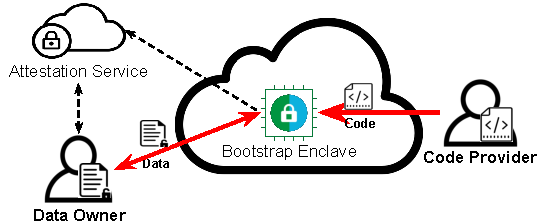
\includegraphics[scale=0.72]{figures/fg-deflection-model.pdf}}
\caption{The \textsc{Deflection} model}\label{fg-cat}
\vspace{-10pt}
\end{figure}
%\weijie{a new figure, to show the trust chain}

%\vspace{3pt}\noindent\textbf{The CAT model}.
\subsection{The Delegation Model}

%The interactions among 4 parties are described as follows.

\vspace{3pt}\noindent\textbf{Attestation service}. Attestation \DIFdelbegin \DIFdel{service }\DIFdelend \DIFaddbegin \DIFadd{Service (AS) }\DIFaddend assists in the remote attestation process by helping the data owner verify the quote generated by an enclave, as performed by the Intel attestation service for SGX. 

%We assume a standard IAS as in Intel's attestation model who verifies the quote and generates the attestation report. 

\vspace{3pt}\noindent\textbf{Bootstrap enclave}. The bootstrap enclave is a built-in control layer on the software stack, hosted by the code provider or a third party cloud  (see Figure~\ref{fg-cat}). Its code is public and initial state is measured by hardware for generating an attestation quote, which is later verified by the data owner with the help of the AS. This software layer is responsible for establishing security channels with enclave users, authenticating and dynamically loading the binary of the target program from the code provider and data from its owner. \DIFdelbegin \DIFdel{Further it }\DIFdelend \DIFaddbegin \DIFadd{It further }\DIFaddend verifies the code to ensure its compliance with predefined security policies before bootstrapping the computation. During the computing, it also controls the data entering or exiting the enclave, e.g., through SGX ECalls/OCalls to perform data sanitization.
    % I want to demonstrate: the loaded code is not allowed to perform OCALL and the ECALL will not reach the loaded code directly. The interfaces are controlled by the bootstrap enclave.

\vspace{3pt}\noindent\textbf{Data owner}. The data owner uploads sensitive data (e.g., personal images) to use in-enclave services (e.g., an image classifier) and intends to keep her data secret during the computation. To this end, the owner runs a remote attestation with the enclave to verify the code of the bootstrap enclave, and sends in data through a secure channel only when convinced that the enclave is in the right state so expected policy compliance check will be properly performed on the target binary from the code provider. 
\ignore{
Note that here we only consider the scenario that the data owner is the only recipient of the output of the enclave service, though the CAT model can be extended to support the application involving multiple data owners and a separate data user.  
}
%Note that there could be more than one data owner to provide data.  


%Depending on applications, there could be more than one owners to send in data. who feed data into the enclave and would like to keep the data from leaking out of the enclave. For this purpose they initiate a remote attestation by sending an attestation request challenge to the enclave developer, inspect and verify the code of the bootstrap enclave by checking the remote attestation report. If they are convinced the bootstrap enclave can guarantee the predefined policies are applied to the loaded code, they can send the data (in encrypted form) to the bootstrap enclave.

\vspace{3pt}\noindent\textbf{Code provider}. The code provider (owner) can be the service provider, and in this case, her target binary (the service code) can be directly handed over to the bootstrap enclave for compliance check. 
%In general, however, the code provider is a different party and may not trust the cloud platform. 
So, similar to the data owner, she can also request a \revise{flexible/portable} remote attestation to verify the bootstrap enclave before delivering her binary to the enclave for a compliance check. 

\DIFaddbegin \vspace{3pt}\noindent\textbf{\DIFadd{Key agreement procedure}}\DIFadd{.
Both parties, a service provider (data owner) and a remote user (code provider), inspect and agree on the implementation details of the bootstrap enclave. The data owner and the code provider can both attest that the bootstrap loader is correctly running on SGX platforms using remote/local attestation. In particular, data owner and code provider both generate a measurement of the bootstrap enclave, which acts as the trust anchor of their agreement and is required for verification during SGX remote/local attestation.
}

\DIFadd{After the two attestations are done and shared session keys are negotiated by Diffie–Hellman key exchange, all messages can be transferred through the two trusted channels.
Since the data owner already knows the measurement/hash of the service code. The bootstrap enclave first extracts and verifies the measurement/hash of the service code, and then sends the measurement/hash to the data owner. After the user is sure about the authenticity of the service code, she can begin to feed data into the service.
}

\DIFaddend % for 11 page limit
\ignore{
\vspace{3pt}\noindent\textbf{Use Cases}.
%\weijie{other portable usage, e.g., enclave migration}
For the example in the introduction, through CAT, a  pharmaceutical company can run its proprietary algorithm inside an enclave hosting patient medical records, without exposing the algorithm but can still ensure the hospital (the data owner) the compliance of its data use with the hospital's privacy policy. As an example, the CAT model can enable a more privacy-preserving credit evaluation service, in which a customer's transactions are only exposed to an enclave running the credit evaluation code in compliance with a set of public privacy-protection rules (such as GDPR).
We consider confidential computing as a service (\textit{CCaaS}) as a privacy extension of today's online data processing services like machine-learning as a service~\cite{russinovich2017introducing}. CCaaS is hosted by the party that operates its own target binary on the data provided by its owner (e.g., an online image classifier to label uploaded user photos). \textit{The outcome of the computation will be sent back to the data owner}. Here, the target binary cannot be released for verification so needs to go through an in-enclave compliance check.
\weijie{code vetting}
}



\ignore{
\vspace{2pt}\noindent\textbf{Sensitive genome data analysis}. Since genetic and health information is extremely sensitive, users may not feel comfortable with the company keeping their data. Meanwhile, a bio-tech companies that owns the intellectual property of its technology would like to use a confidential algorithm to process the data. In this scenario, people upload their genes for private computation that can be outsourced and protected in CAT-SGX. Basic sequence generation and alignment algorithms can be widely used in reads mapping and GATK softwares, while a sequence generation/alignment algorithm often takes strings as an input while gives out strings as ouput. During the confidential service, CAT-SGX keeps the label of genes and the intermediate variables, then forwards the result back to the user when finished. 


\vspace{2pt}\noindent\textbf{Personal credit score analysis}. Consider a bank or a credit agency that provides different levels of loan transactions before it evaluates each applicant's financial status. Then, credit scoring is a typical application that needs to be protected more carefully - both the credit card holder's cost calendar and card issuer's scoring algorithm need to be kept secret. 
The input file contains users' history records and the output is a prediction whether the bank should approve the next transaction. In this case, CAT-SGX only allows two-bytes output to in the score and one bit (bool) to indicate whether the bank should approve or decline the transaction.
}


%could verify the code of the bootstrap enclave through remote attestation. Only after they believe that the bootstrap enclave guarantees the predefined policies, the code can be sent into the bootstrap enclave secretly.

% In order to solve the problem of private algorithm and data, both distrustful parties could utilize secure hardware enclaves. Here, we give some definitions. A Data Owner (DO) refers to an entity who has privacy-sensitive inputs. A Service Provider (SP) refers to an entity who has private algorithms. A Enclave Developer (ED) works with the hardware owner (HO), managing its own computational power and maintaining the hardware.



\subsection{Guidelines}
\label{subsec-challenges} 

To instantiate a \textsc{Deflection} System on a real-world TEE such as SGX, we expect the following requirements to be met by the design: 

%At the core of instantiating the CAT model is the design of the bootstrap enclave who is responsible for enforcing the privacy and security policies. We list the design goals to enable a secure and efficient bootstrap enclave.

\vspace{3pt}\noindent\textbf{Minimizing TCB and resource consumption}.\label{challenge-tcb}\label{challenge-size} 
Today's TEEs operate under resource constraints.  Particularly, SGX is characterized by \DIFdelbegin \DIFdel{limited EPC}\DIFdelend \DIFaddbegin \DIFadd{a limited Enclave Page Cache (EPC)}\DIFaddend . To maintain reasonable performance, we expect the software stack of the \textsc{Deflection} model \DIFdelbegin \DIFdel{controls }\DIFdelend \DIFaddbegin \DIFadd{to control }\DIFaddend its resource use. The bootstrap enclave is responsible for enforcing security and privacy policies and for controlling the interfaces that import and export code/data for the enclave. So it is critical for trust establishment and needs to be kept as compact as possible for code inspection or verification~\cite{mccune2008flicker}.  

\vspace{3pt}\noindent\textbf{Controlling portable code loading}.\label{challenge-dep} The target binary is dynamically loaded and inspected by the bootstrap enclave. However, the binary may further sideload other code during its runtime. 
%Some TEE hardware, SGX in particular, does not allow dynamic change to enclave page's RWX properties. 
So the target binary, itself loaded dynamically, is executed on the enclave's heap space. Preventing it from sideloading requires a data execution prevention (DEP) scheme to guarantee the W $\oplus$ X privilege.

%current SGX hardware, dynamically changing the RWX properties of enclave pages are not supported. So the loaded program will be executed on enclave's heap space, and we need a fine data execution prevention (DEP) scheme to guarantee W $\oplus$ X privilege.% and isolates security-sensitive data structures from adversaries.

    % Leveraging PCC on program verification could greatly relieve the burden on the code consumer's side - PCC moves most daunting work to the code producer. However, we still need to further improve the performance of our design because there are too many objects (memory write operations and indirect branches) that we have to analyze.
    %\textit{Limited computing resources}. SGX has only a limited memory space. Considering the typical usages of SGX would also occupy tens of MBs of memory, doing confidentiality analysis would be a difficult task. The TCB of the whole verifying system inside the enclave should be as thin as possible. 
    %Also, how to reduce the amount of proof size for verification needs to be dealt with. Thus, we should build a lightweight checking scheme to simplify the verifier/checker with the help of the compiler, and optimize the compiler to generate as less proof as possible.

\vspace{3pt}\noindent\textbf{Preventing malicious control flows}.\label{challenge-cfi} 
Software stack should be designed to prevent the code from escaping policy enforcement by redirecting its control flow or tampering with the bootstrap enclave's critical data structures. Particularly, previous work shows that special instructions like ENCLU could form unique gadgets for control flow \DIFdelbegin \DIFdel{redirecting}\DIFdelend \DIFaddbegin \DIFadd{redirection}\DIFaddend ~\cite{biondo2018guard}, which therefore need proper protection. 

\vspace{3pt}\noindent\textbf{Minimizing performance impact}.\label{challenge-perf} In all application scenarios, the data owner and the code provider expect a quick turnaround from code verification. Also the target binary's performance should not be significantly undermined by the runtime compliance check. 

%It is also important in many scenarios to reduce the time for checking the policy compliance and to induce low run-time overhead for the computation. 



\subsection{Threat Model}
\label{subsec-threat}

The delegation model is meant to establish trust between the enclave and the code provider, as well as the data owner, under the following assumptions: 

%To demonstrate how to instantiate the CAT model, in the rest of the paper we consider a specific application scenario, i.e., privacy preserving online data processing (Scenario 1 in Sec.~\ref{subsec-scenarios}). As shown in Sec.~\ref{subsec-motivation}, many real world privacy preserving data processing tasks fall into this scenario. As described earlier for Scenario 1, the user (i.e., the data provider) submits her sensitive data to a service provider (i.e., the code owner) for data processing tasks. In our threat model, we make the following assumptions.

\vspace{2pt}\noindent$\bullet$ We do not trust the service code (target binary) and the platform hosting the enclave. In CCaaS, the platform may deliberately run vulnerable code to exfiltrate sensitive data, by exploiting \DIFdelbegin \DIFdel{the }\DIFdelend known vulnerabilities during \DIFaddbegin \DIFadd{the }\DIFaddend computation. 
%We trust data owner.
%The binary can also leak the data through a covert channel (e.g., page fault~\cite{xu2015controlled}).   

%\hongbo{Out of our scope: data owner infer code by inspecting the output}

%\vspace{2pt}\noindent$\bullet$ We assume the data owner (service user) is benign. Data provider would not use specially-crafted data to learn about the operation of the secret code given the output.

%\weijie{we do not consider other kinds of leakage such as DOP attack? or the data owner would try to steal the service code. }


%The service provider may (intentionally) write vulnerable service code which causes the leakage of the users' data, e.g., the enclave may be compromised by another user with memory corruption attacks. The service code can even collude with the SGX-enabled platform owned and controlled by the attacker, e.g., through covert channels (such as page faults etc.). 

\ignore{
\weijie{out of scope} \vspace{2pt}\noindent$\bullet$ Our current implementation of CAT-SGX focuses on privacy compliance at this time, and we do not examine the functionalities of the target binary. We believe the design can be extended to ensure other properties of the program. Also, although TEE is designed to prevent information leaks to the untrusted OS, denial of service can still happen, which is outside the scope of the model. }


%\vspace{2pt}\noindent$\bullet$ Under the untrusted service provider, \revise{our method can be used to guarantee the correctness of the computation. However, since the current implementation of CAT-SGX is not meant to inspect the functionalities of the target binary, we only care about the privacy compliance at this time.}
%Since the service provider is untrusted, our design does not intend to guarantee the correctness of the results returned to the users. The service users can refuse to pay for the service or turn to other service providers if the results are inferior. This is similar as Denial-of-Service (DoS) attacks which are also out of scope.

\vspace{2pt}\noindent$\bullet$ We assume that the code of the bootstrap enclave can be inspected to verify its functionalities and correctness.  Also we consider the TEE hardware, its attestation protocol, and all underlying cryptographic primitives to be trusted.  


\vspace{2pt}\noindent$\bullet$ Our model is meant to protect data and code against different kinds of information leaks, not only explicit but also implicit.  However, side channel in a user-land TEE (like SGX) is known to be hard to eliminate, which all existing SGX runtimes (including container~\cite{arnautov2016scone}, sandbox~\cite{hunt2018ryoan}, interpreter~\cite{wang2019towards} and others) fail to address. So our design for instantiating the model on SGX (Section~\ref{subsec-policies}) just aims to make the first step towards closing of this attack surface, mitigating some types of side-channel threats.  

%Besides, we assume the bootstrap enclave code can be inspected (or formally verified) by the users through remote attestation, so that it is trusted to be functional as designed. We trust the SGX hardware and the Intel's attestation protocol as well as the cryptographic algorithms underneath. The mutual authentication between the users and service provider is orthogonal to the design and is omitted in the paper.

%\weijie{The data provider is relatively benign and won't do things that jeopardizes data privacy of its own, e.g., sending some malicious input (triggering unexpected attacks) into the code. }

% =====================================================================

    
    
    
    
    
    
    
    
%---------------------------------------------------------------------------------------------------------------


\ignore{

\section{Confidential Attestation}\label{sec-CAT}
%\vspace{3pt}\noindent\textbf{Motivating Example}.

\subsection{Motivating Example}\label{subsec-motivation}

Consider a company providing data-processing services, such as image editing (Pixlr), tax preparation (TurboTax), personal health analysis (23andMe) and deep learning inference as a service, the users need to disclose their sensitive data, such as images, tax documents, and health data, to leverage the convenience and expertise of these services. The user can acquire the data processing performed inside an SGX enclave, and further, verify the enclave code through remote attestation to prevent unintended data disclosure. However, the service provider may not want to disclose the enclave code to the user for verification due to intellectual property reasons, in which case the SGX attestation model fails to fulfill the privacy requirement of both the user (i.e. the data owner) and the service provider.

In this section, we propose the \textit{Confidential ATtestation} (CAT) model to allow the data owner to verify that the enclave code satisfies predefined privacy and security policies without undermining the privacy of the enclave code.
We enumerate several application scenarios that could benefit from the proposed CAT model. We will further list the design goals in designing a practical CAT model in the context of Intel SGX, as well as the threat model considered in the paper. 

%Aiming to complete a system that can flexibly verify whether the code leaks data on SGX platforms, we propose Confidential Attestation. This technology can be used in different situations.
%In particular, we will enumerate all technical challenges needed to be overcome during building such a system, and will elaborate the threat model during achieving all purposes of our design.

%The service provider often has secret algorithms or business logic that can not be exposed. As an entity that needs/should to compute a secret value, it may be willing to secure the private algorithm during delivery. Meanwhile, the service provider could sell the intelligent property to a user who wants to process the secret data for a trustworthy and correct result.

%From Intel: With a bit of hand waving one could envision a 'proprietary' code module which is symmetrically encrypted and thus protected outside the context of an enclave.   In this model one still needs a 'bootstrap' enclave which has to have access to the encryption material needed to authenticate and decrypt the code/data which is being dynamically loaded.  That leaves you back at the need to establish a security context between the 'bootstrap' enclave and the authority/context which has prepared the protected material for ingress into the enclave.

%\vspace{3pt}\noindent\textbf{The CAT model}.
\subsection{The CAT model}

There are 4 parties involved in the CAT model.

%\vspace{3pt}\noindent\textbf{The enclave developer}. It provides the code of the bootstrap enclave (see below), which can be made public. Then it conducts the Intel's attestation model as an ISV on behalf of the data providers and the code providers (see below). Specifically it accepts the attestation request challenge and forwards it to the enclave, then it forwards the quotes to the IAS to get the attestation report. At last it forwards the attestation report to the party who initiates the remote attestation.
%\hongbo{Why should enclave developer appears in the CAT model? During the lifetime of the bootstrap enclave/service code, the developer will not be in the computation task. The attestation will be done by the bootstrap enclave(not the developer). Maybe platform is more appropriate}

\vspace{3pt}\noindent\textbf{The IAS}. We assume a standard IAS as in Intel's attestation model who verifies the quote and generates the attestation report. 

\vspace{3pt}\noindent\textbf{The bootstrap enclave}. It is the initial code built into the enclave, which is measured by the hardware to generate the measurement report. It is responsible to authenticate and dynamically load the code and data for the computation to be conducted. It then verifies the code and data is compliant to predefined policies and bootstraps the computation. It is responsible for establishing protected communication channels, and audit the ECalls/OCalls to sanitize the data sent to or received from outside of the enclave.
    % I want to demonstrate: the loaded code is not allowed to perform OCALL and the ECALL will not reach the loaded code directly. The interfaces are controlled by the bootstrap enclave.

\vspace{3pt}\noindent\textbf{The data providers}. Depending on the applications, there can be multiple data providers who feed data into the enclave and would like to keep the data from leaking out of the enclave. For this purpose they initiate a remote attestation by sending an attestation request challenge to the enclave developer, inspect and verify the code of the bootstrap enclave by checking the remote attestation report. If they are convinced the bootstrap enclave can guarantee the predefined policies are applied to the loaded code, they can send the data (in encrypted form) to the bootstrap enclave.

\vspace{3pt}\noindent\textbf{The code providers}. Similar as the data providers, code provider/owner could verify the code of the bootstrap enclave through remote attestation. Only after they believe that the bootstrap enclave guarantees the predefined policies, the code can be sent into the bootstrap enclave secretly.

% In order to solve the problem of private algorithm and data, both distrustful parties could utilize secure hardware enclaves. Here, we give some definitions. A Data Owner (DO) refers to an entity who has privacy-sensitive inputs. A Service Provider (SP) refers to an entity who has private algorithms. A Enclave Developer (ED) works with the hardware owner (HO), managing its own computational power and maintaining the hardware. 
\subsection{Application Scenarios}\label{subsec-scenarios}

In the following, we enumerate several application scenarios that could benefit from the proposed CAT model. 
%\weijie{code and data should be encrypted sometimes for such three scenarios.}
%\vspace{3pt}\noindent\textbf{Examples.}

\begin{figure}[htbp]
\begin{center}
\centerline{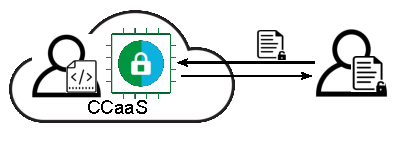
\includegraphics[scale=0.72]{figures/fg-scenario-1.pdf}}
\caption{Scenario 1}\label{fg-scenario_1}
\end{center}
\end{figure}


\weijie{change the name of scenarios to: confidential computing as a service, confidential data as a service, etc.}

\vspace{3pt}\noindent\textbf{Scenario~\ref{fg-scenario_1}: Privacy preserving online data processing service}. As the motivating example (Sec.~\ref{subsec-motivation}) shows, the data-processing service (i.e., the bootstrap enclave) is hosted on an SGX-enabled platform owned by the service provider (i.e., the code provider), while the user (i.e., the data provider) sends her encrypted sensitive data for processing. The result will be sent back to the data provider (possibly in encrypted form). As such, the user would like that the bootstrap enclave can enforce the security policy that her data would never leave the enclave.
%\hongbo{In these figures, is enclave developer denotes the cloud? I think it should be SGX-enabled platform.}

\begin{figure}[htbp]
\centerline{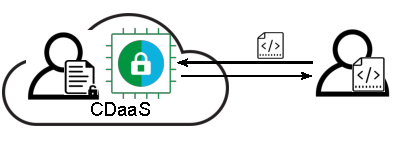
\includegraphics[scale=0.72]{figures/fg-scenario-2.pdf}}
\caption{Scenario 2}\label{fg-scenario_2}
\end{figure}

\vspace{3pt}\noindent\textbf{Scenario~2: Privacy preserving online data as a service}. In this scenario, the data-as-a-service (i.e., the bootstrap enclave) is hosted on an SGX-enabled platform owned by the data provider. A user (i.e., the code owner) who would like to conduct computation (such as genome analysis) on the data sends her sensitive code via a secure channel . The result will be sent back to the code provider (possibly in encrypted form). As such, the user would like that the bootstrap enclave can enforce the security policy that the data used are not faked or impure, and her code will not be unintended redirected so that the result is reliable.

\begin{figure}[htbp]
\centerline{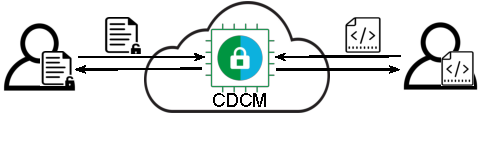
\includegraphics[scale=0.72]{figures/fg-scenario-3.pdf}}
\caption{Scenario 3}\label{fg-scenario_3}
\end{figure}

\vspace{3pt}\noindent\textbf{Scenario~3: Privacy preserving online data market}. In this scenario, a data market platform (i.e., the bootstrap enclave) is hosted on a third party.
%besides the data user (i.e., the code provides) and data owner (i.e., the data providers). 
The data owner uploads her encrypted data to the platform so that she gets paid if the data is used. The data user uploads her code (e.g. genome analysis) also secretly to be computed on people's data satisfying some preset conditions. As such, besides enforcing the confidentiality of both the code and data, the data owner would like to ensure that she gets paid as long as the data is used, while the data user want to ensure that she's not overcharged.

Besides the above scenarios, CAT may be used in more applications, such as privacy preserving smart contract, etc.

%\vspace{3pt}\noindent\textbf{Technical challenges}.
\subsection{Design goals}
\label{subsec-challenges} 
At the core of instantiating the CAT model is the design of the bootstrap enclave who is responsible for enforcing the privacy and security policies.
We list the design goals to enable a secure and efficient bootstrap enclave.

\vspace{3pt}\noindent\textbf{Minimizing the Trusted Computing Base (TCB)}.\label{challenge-tcb} 
    In the CAT model the bootstrap enclave is responsible for enforcing the security and privacy policies and to control the interfaces between the loaded code/data and outside of the enclave. The trust built by the CAT model will collapse once it is compromised. It is essential to control the size of the bootstrap enclave and that it can be (formally) verified in the future.

\vspace{3pt}\noindent\textbf{Reducing the memory consumption}.\label{challenge-size} 
    There are limited EPC memory that could be used by the SGX enclave. Considering that the data-processing computation itself consume considerable memory, the design needs to reduce the memory cost adequately.

\vspace{3pt}\noindent\textbf{Confining the (untrusted) loaded code}.\label{challenge-dep} On current SGX hardware, dynamically changing the RWX properties of enclave pages are not supported. So the loaded program will be executed on enclave's heap space, and we need a fine data execution prevention (DEP) scheme to guarantee W $\oplus$ X privilege.% and isolates security-sensitive data structures from adversaries.

    % Leveraging PCC on program verification could greatly relieve the burden on the code consumer's side - PCC moves most daunting work to the code producer. However, we still need to further improve the performance of our design because there are too many objects (memory write operations and indirect branches) that we have to analyze.
    %\textit{Limited computing resources}. SGX has only a limited memory space. Considering the typical usages of SGX would also occupy tens of MBs of memory, doing confidentiality analysis would be a difficult task. The TCB of the whole verifying system inside the enclave should be as thin as possible. 
    %Also, how to reduce the amount of proof size for verification needs to be dealt with. Thus, we should build a lightweight checking scheme to simplify the verifier/checker with the help of the compiler, and optimize the compiler to generate as less proof as possible.

\vspace{3pt}\noindent\textbf{Preventing malicious control flows}.\label{challenge-cfi} 
    Previous work shows that special instructions in SGX like ENCLU would make unique gadgets for control flow redirecting attacks.
    Since the loaded code can not be trusted, the design needs to prevent code from escaping the policy enforcement by redirecting the control flow and tampering the security-sensitive data structures of the bootstrap code.
    %code control flow hijacking techniques to compromise
    %Although we can use SGX's Remote Attestation (RA) to ensure the integrity of our verifier/checker, there can be many control flow hijacking techniques to compromise the verifier and bypass the checks. 
     %So a more thorought CFI policies should be executed to prevent various malicious control flow redirecting within the untrusted service code.
   % \item \textit{Dynamic code loading and data execution protection}.\label{challenge-3} Normal x86 binaries built outside the enclave can not be simply running inside, due to restrictions caused by Intel SGX. To enable verifying the service provider’s code yet without knowing the code itself, a loader in enclave could be built so that the loader do the verification and be attested by remote user using Intel SGX’s RA. But how to design a practical loader for loading/relocating binaries dynamically? Therefore, we need a good way to assemble the binary using our code generator and load the relocatable file after the loader is initialized. In the meantime, since the loaded program will be executed on enclave's heap space, we also need a fine DEP plan to guarantee W $\oplus$ X privilege and isolates security-sensitive data structures from adversaries.

\vspace{3pt}\noindent\textbf{Performance considerations}.\label{challenge-perf} It is also important in many scenarios to reduce the time for checking the policy compliance and to induce low run-time overhead for the computation. 

%\vspace{3pt}\noindent\textbf{Threat model}. 
\subsection{Threat model}
\label{subsec-threat}
%In this paper we assume a strong adversary in the CAT model, i.e., the code providers and data providers do not trust each other. 
To demonstrate how to instantiate the CAT model, in the rest of the paper we consider a specific application scenario, i.e., privacy preserving online data processing (Scenario 1 in Sec.~\ref{subsec-scenarios}). As shown in Sec.~\ref{subsec-motivation}, many real world privacy preserving data processing tasks fall into this scenario. 
%We stress that instantiating the CAT model in the other application scenarios are important future works.
As described earlier for Scenario 1, the user (i.e., the data provider) submits her sensitive data to a service provider (i.e., the code owner) for data processing tasks. In our threat model, we make the following assumptions.

%Before the discussion of how we design a practical Privacy-preserving TEE, a threat model could be built for better define the scope of the problem we need to solve. 

\vspace{2pt}\noindent$\bullet${ The service code and the SGX-enabled host platform are not trusted.} The service provider may (intentionally) write vulnerable service code which causes the leakage of the users' data, e.g., the enclave may be compromised by another user with memory corruption attacks. The service code can even collude with the SGX-enabled platform owned and controlled by the attacker, e.g., through covert channels (such as page faults etc.). 

%to do whatever they can to steal the data owner’s sensitive information. But we believe in Intel SGX and its RA protocol, which could be seen as a trusted third party.


%\hongbo{Do we need to mention the cloud computation platform is also untrusted?}
\vspace{2pt}\noindent$\bullet$ Since the service provider is untrusted, our design does not intend to guarantee the correctness of the results returned to the users. The service users can refuse to pay for the service or turn to other service providers if the results are inferior. This is similar as Denial-of-Service (DoS) attacks which are also out of scope.

\vspace{2pt}\noindent$\bullet$ Besides, we assume the bootstrap enclave code can be inspected (or formally verified) by the users through remote attestation, so that it is trusted to be functional as designed. We trust the SGX hardware and the Intel's attestation protocol as well as the cryptographic algorithms underneath. The mutual authentication between the users and service provider is orthogonal to the design and is omitted in the paper.

%\vspace{2pt}\noindent$\bullet$\textit{The data is encrypted and intact before the enclave starts to run the data-processing application.} Intel SGX and its built-in toolsets can make both the service provider’s code and user’s data loaded into an enclave securely via RA and key exchange. And if necessary, service provider could apply some differential privacy techniques and add certain noisy to protect the data from inference attacks.
    %As discussed earlier the loaded code cannot perform Ocalls directly, and we assume that all ECalls/OCalls will be audited by the bootstrap enclave. 
    %Since all the bridge functions should be public for normal use, it makes sense that we can make such assumption in this service-oriented scenarios. And if necessary, service provider could add certain noisy to protect the data from inference attacks.
    %\item Currently, we do not consider side channels or covert channels between the enclave code and the outside world. In this paper, we are confined to verifying simple confidentiality properties and do not handle complex adversary models like those involving side-channels.\wenhao{remove this item}
}

    
    
\section{Design}\label{sec-design}
%\section{Design}\label{sec-design}



%As described in Sec.~\ref{sec-CAT}, a confidential attestation process encompasses a standard Intel attestation to attest the bootstrap enclave and establish a secure communication channel. If they are convinced that the bootstrap enclave can enforce the desired security policies, the data or code providers can send the data and code (in encrypted form) to the bootstrap enclave. 

In this section we present our design, which elevates the SGX platform with the support for the \textsc{Deflection} model. This is done using an in-enclave software layer -- the bootstrap enclave running the code consumer and an out-enclave auxiliary -- the code generator. 
\DIFdelbegin \DIFdel{Following we first describe the general idea behind our design and then elaborate the policies it supports, its individual components and potential extension.     
}\DIFdelend %DIF >  Following we first describe the general idea behind our design and then elaborate the policies it supports, its individual components and potential extension.     


%under the privacy preserving data processing scenario. In this setting, the service user (i.e., the data owner) communicates with the remote data processing service with encrypted messages for uploading her data and receiving the results.
%sends and receives  from remote parties. The service provider is with the infrastructure's side so that the code can be conveyed directly into the bootstrap enclave. 
%To minimize the size of the bootstrap enclave, the design borrows the idea of PCC and consists of an untrusted code producer outside the enclave, and a trusted code consumer inside.
%Sec.~\ref{subsec-threat} presents the threat model. 
%Sec.~\ref{subsec-policies} presents the categorized security policies enforced by the bootstrap enclave. Sec.~\ref{subsec-producer} and Sec.~\ref{subsec:verify} presents how the policies can be enforced and verified with the cooperative design of the code producer and code consumer. We will discuss how to extend the design to other scenarios with carefully crafted security policies in Sec.~\ref{subsec:morescenario}. 


%In this section we present our design for realizing the CAT model under the privacy preserving data processing scenario. In this setting, the service user (i.e., the data owner) communicates with the remote data processing service with encrypted messages for uploading her data and receiving the results.
%sends and receives  from remote parties. The service provider is with the infrastructure's side so that the code can be conveyed directly into the bootstrap enclave. To minimize the size of the bootstrap enclave, the design borrows the idea of PCC and consists of an untrusted code producer outside the enclave, and a trusted code consumer inside.Sec.~\ref{subsec-threat} presents the threat model. Sec.~\ref{subsec-policies} presents the categorized security policies enforced by the bootstrap enclave. Sec.~\ref{subsec-producer} and Sec.~\ref{subsec:verify} presents how the policies can be enforced and verified with the cooperative design of the code producer and code consumer. We will discuss how to extend the design to other scenarios with carefully crafted security policies in Sec.~\ref{subsec:morescenario}. 


%with little or no modification since the code generator and the policy-compliance verifier can work perfectly independently and have no impact on one another.




\subsection{\DIFaddbegin \DIFadd{Architecture }\DIFaddend Overview}
\label{subsec-overview}

\DIFdelbegin %DIFDELCMD < \noindent%%%
\textbf{\DIFdel{Idea}}%DIFAUXCMD
\DIFdel{. Behind the design of }\textsc{\DIFdel{Deflection}} %DIFAUXCMD
\DIFdel{is the idea of PCC, which enables efficient in-enclave verification of }%DIFDELCMD < \revise{mobile code with proof}%%%
\DIFdel{. A direct application of the existing PCC techniques, however, fails to serve our purpose, as mentioned earlier, due to the huge TCB introduced, the large proof size and the exponential time with regards to the code size for proof generation. To address these issues, we design a lightweight 
approach with an untrusted code producer and a trusted code consumer running inside the bootstrap enclave. The producer compiles the source code of the target program with necessary libraries (for service providing), generates a list of its indirect jump targets, and instruments it with security annotations (in assembly with structured inline guards) for runtime mediation of its control flow and key operations, in compliance with security policies. The list and security annotations constitute a ``proof'', which is verified by the consumer (according to certain formats) after loading the code into the enclave and before the target binary is activated. 
}\DIFdelend %DIF >  \noindent\textbf{Idea}. Behind the design of \textsc{Deflection} is the idea of PCC. The code producer (in Figure~\ref{fg-overview}) compiles the source code of the target program with necessary libraries (for service providing), generates a list of its indirect jump targets, and instruments it with security annotations (in assembly with structured inline guards) for runtime mediation of its control flow and key operations, in compliance with security policies. The list and security annotations constitute a ``proof'', which is verified by the consumer after loading the code into the enclave and before the target binary is activated. 
\DIFaddbegin 

\DIFaddend %\weijie{proof/annotation: assembly with certain format/inline guards, inspired by the typed x86 assembly}

%The overview design is derived from the original PCC idea while we have simplified it for our own purpose. The illustration of our design lists all components that are divided into two parts, trusted part and untrusted part. In our new PCC-based system, the proof is generated from the outside of the enclave during the compiling and can be verified at runtime inside. The inside verifier can cooperate with the outside compiler to make the verifier as lightweight as possible, using static verification of dynamic checks.

%A common method to enable efficient verification of the code properties within the bootstrap enclave is to use PCC. We find, however, applying traditional PCC schemes directly to the CAT model is impractical due to the following reasons: (1) Traditional PCC schemes induce huge TCB, including the VC generator with an intermediate  language interpreter/compiler, or a virtual machine that can support runtime proof checking. (2) In traditional PCC schemes, the proof size is usually large. (3) Although the procedure of generating proof runs outside the enclave and is not trusted, it usually takes exponential time with respect to the code size and may take too long for real world data processing computations.

\begin{figure}[htbp]
%\centerline{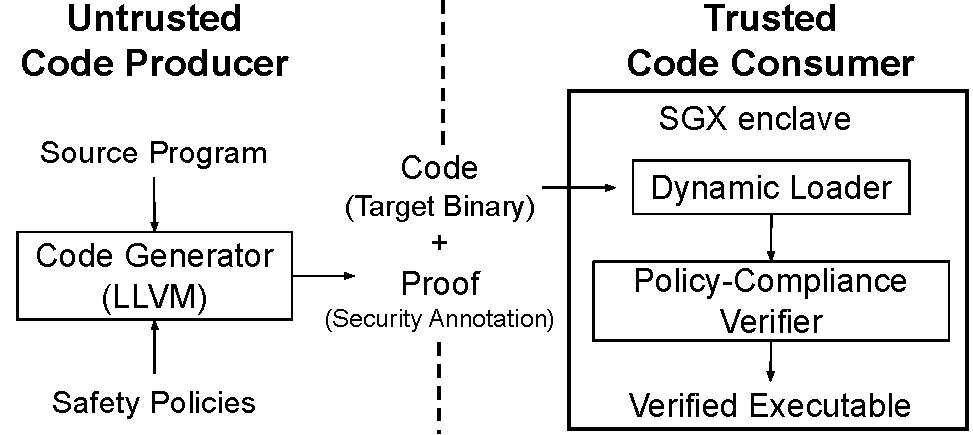
\includegraphics[scale=0.45]{figures/arch_overview.pdf}}
\centerline{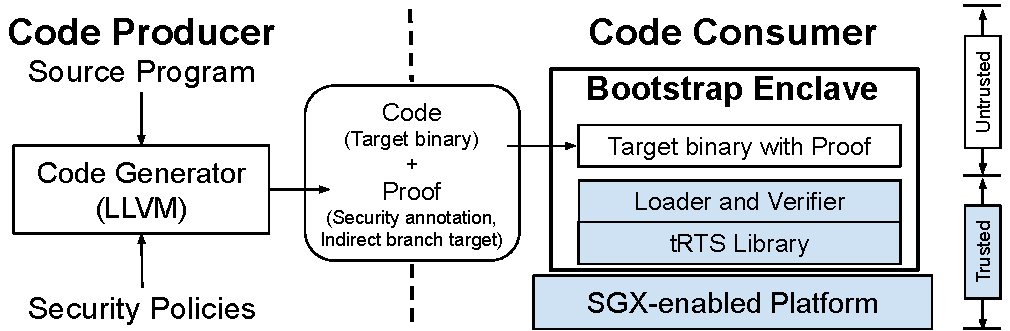
\includegraphics[scale=0.45]{figures/fg-bootstrap-layer.pdf}}
\caption{System overview}\label{fg-overview}
\vspace{-12pt}
\end{figure}

\DIFdelbegin %DIFDELCMD < \vspace{3pt}\noindent%%%
\textbf{\DIFdel{Architecture}}%DIFAUXCMD
\DIFdel{. The architecture of is illustrated in Figure~\ref{fg-overview}. }\DIFdelend The code generator and the binary\DIFdelbegin \DIFdel{and proof it produced }\DIFdelend \DIFaddbegin \DIFadd{/proof it produces }\DIFaddend are all considered untrusted. \DIFdelbegin \DIFdel{Only }\DIFdelend \DIFaddbegin \DIFadd{The code consumer }\DIFaddend in the TCB is \DIFdelbegin \DIFdel{the code consumer }\DIFdelend with two components: a dynamic-loader operating a rewriter for re-locating the target binary, and a proof verifier running a disassembler for checking the correct instrumentation of security annotations. These components are all made public and can therefore be measured for a remote attestation (Section~\ref{subsec:ra-impl}). They are designed to minimize their code size, by moving most workload to the code producer. 

%\weijie{will unify them all into `verifier'}

%In traditional PCC framework, the VCGen often exists as a compiler~\cite{colby2000certifying,leroy2006formal} or a sandbox~\cite{pirzadeh2010extended}, which is too heavy for limited executive resources. So here, we build our own lightweight PCC system to verify if a cloud service would leakage user’s data. Generally, we provide a code transformer for service code which needs to be verified, and a secure enclave for executing the verified service code. 

%The only TCB in our design is the verifier code inside the enclave, including the dynamic-loader, the disassembler/rewriter (for rewritting structured guards), and the proof verifier (for checking verification hints). On the other hand, the whole trusted code consumer can be remotely attested (in Subsection~\ref{subsec-dynamicloader}), which can indirectly protect the integrity of for code provider, as well as the isolate valuable implementation detail from be accessed.

%As mentioned above, to facilitate PCC framework working well in SGX and to make PCC more efficient, specifically to reduce the size of code consumer side, we move as much proof generation workload as possible to the code producer side, and leave as few verification workload as possible to the inside of the enclave.

\begin{figure*}[htbp]
\centerline{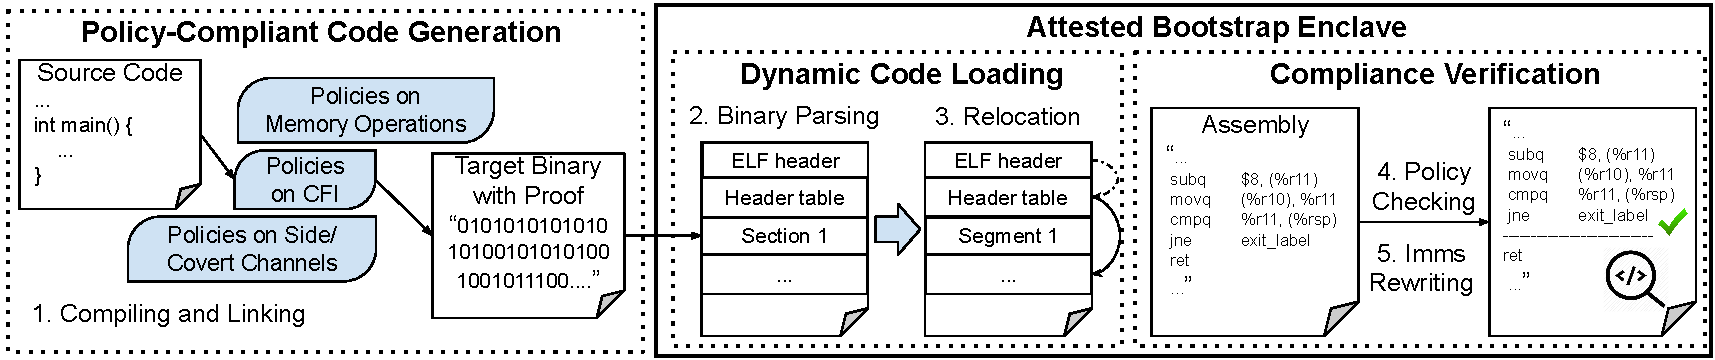
\includegraphics[scale=0.5]{figures/fg-workflow.pdf}}
\caption{Detailed framework and workflow}\label{fg-workflow}
%\wenhao{Typo: Attestated Bootstrap Enclave}
%\weijie{done. Thanks!}
\vspace{-15pt}
\end{figure*}
%\weijie{need some changes on the figure}

 We present the workflow of \textsc{Deflection} in Figure~\ref{fg-workflow}. %DIF < Unlike the typical interaction between the producer and consumer, the workflow encompasses several steps. 
The target program (the service code) is first instrumented by the code producer, which runs a customized LLVM-based compiler (step 1). 
%Then on the code consumer side, the loader source code and the verifier source code are compiled with SGX SDK to build the bootstrap enclave binary (step 3). 
Then the target binary with the proof are delivered to the enclave. The code is first parsed (step 2) and then disassembled from the binary's entry along with its control flow traces.
\DIFdelbegin %DIFDELCMD < \revise{After that, the proof with the assembly
%DIFDELCMD < is relocated and activated by the dynamic loader (step 3), further inspected by the verifier and if correct (step 4) before some immdiates being rewriten (step 5).} %%%
\DIFdelend \DIFaddbegin \revise{After that, the proof with the assembly
is relocated and activated by the dynamic loader (step 3), further inspected by the verifier and if correct (step 4) before some immediates being rewriten (step 5).} \DIFaddend Finally, after the bootstrap transfers the execution to the target program, the service begins and policies are checked at runtime.

%\weijie{The description of the steps does not match the steps presented in Figure 3; weird/incorrect sentence construction, typos, inconsistent capitalization of 'Step' (After that, the proof with the assembly inspected by the verifier and if correct (step 3) before some immdiates [sic] being rewriten [sic] (step 4), is further relocated and activated by the dynamic loader (Step 5).}

%Our loader can load and unload code after initialization (step 4), followed by being remote attested (step 5). Moreover, the `code + proof' can be transferred to code consumer where SGX is deployed, waiting for being dynamic loaded and rebased into the enclave (step 6). After being loaded, the verifier will rewrite some key immediate operands (Imm) and finally transfer the execution to the target program (step 7). 

\ignore{
\vspace{3pt}\noindent\textbf{Dynamic Code Loading and Unloading.} \label{subsec-dynamicloader}
%To ensure the bootstrap enclave's code can be completely public and can be attested, we propose a multi-step loader that can load and unload a generated `code + proof' dynamically. Unlike previous work, our proposed solution can resolve the problem that remote attestation conflicts with the dynamic relocation requirement~\cite{seo2017sgx}. Specifically, remote attestation requires code, data and security properties of the enclave to remain unchanged, while executing a private binary code needs relocation for execution, which is a modification to memory distribution. 
%Our proposal is based on the fact that binary code to be verified can not be trusted, so the measurement of the enclave should not include the untrusted code. Therefore, the code to be verified should be dynamically loaded and relocated after the bootstrap enclave is initiated. 
%\weijie{elaborates it later in Section Implementation}
%\vspace{3pt}\noindent\textbf{Separated Linking and Rebasing.} 
In our design, the linking procedures (linking and rebasing) of a target program are separated into both inside and outside the enclave respectively. SGX only accepts that code running inside an enclave is linked against the SGX SDK at build time. For a self-contained function (i.e., one does not use external elements), compiling and sending the bytes of the assembled code is enough. However, if the function uses external elements, a distributed mechanism is needed to map these elements into their corresponding positions at the enclave side. So we use separated linking and rebasing to assemble all the symbols of the entire code (including necessary libraries and dependencies) into one relocatable file (aka. linking), and then parse the symbols and load/relocate the code at runtime inside the enclave (aka. rebasing). Further, during the linkage procedure, we also load and relocate an indirect branch target entry list as part of the proof for later runtime verification.
%Note that legal jump addresses can not be settled until the rebasing procedure is completed because rebasing will modify the addresses of symbols.

The rebasing process starts with the bootstrap enclave receiving the generated binary code through a buffer. The dynamic loader's primary task is to rebase all of its symbols according to information in its relocation table. Therefore, the loader reads relocation tables in the code, updates symbol offsets in its symbol tables, and loads symbols to addresses designated in the relocation table. After rebasing, the detailed memory layout is shown on the right side in Fig.~\ref{fg-dynloader}.
}



%\wenhao{can elaborate on this. The numbers are not in any order}

\subsection{Security Policies}\label{subsec-policies}
%\subsection{Security Policies for the Privacy Preserving Online Data Processing Scenario}\label{subsec-policies}

%Our general goal of defining safety policies is to design a Privacy-preserving TEE prototype on a service-oriented environment for data owner. Here, we make some rules to constrain our design.
Without exposing its code for verification, the target binary needs to be inspected for compliance with security policies by the bootstrap enclave. These policies are meant to protect the privacy of sensitive data, to prevent its unauthorized disclosure. The current design supports following categories. 

%In this scenario, the bootstrap enclave needs to enforce that the data will not be leaked by the untrusted service code, which is not exposed to the data provider. It can be achieved by enforcing several policies as follows. Notably, the policies put some constraints on the service code, yet we make a lot of effort on these constraints to ensure that the code functionality are intact and necessary for the CAT model.

\vspace{3pt}\noindent\textbf {Enclave entry and exit control}. 
\textsc{Deflection} can mediate the content imported to or exported from the enclave, through the ECall and OCall interfaces, for the purposes of reducing the attack surface and controlling information leaks. 
%In CAT’s model, neither the service code nor the infrastructure is under the control of the user, and they may try to steal the user’s secrets by colluding via covert channels.
Another objective here is to mitigate covert channel leaks through the interface between the enclave and the OS, making the attempt to covertly using users’ data to modulate events (e.g., system call arguments, I/O traffic statistics) hard to succeed.
%\weijie{we support multi-use, by cleaning resident data}

%In such service-oriented scenarios, all the bridge functions should be public and attestable for normal use, we should make restrictions on them. The output is to be produced encrypted and the loader must deal with system calls via a trusted Ocall routine. All ECalls/OCalls will be audited and configured correctly by the bootstrap enclave.

\vspace{2pt}\noindent$\bullet$\textit{ P0: Input constraint, output encryption and entropy control}.
We restrict the ECall interfaces to just serving the purposes of uploading data and code, which perform authentication, decryption and optionally input sanitization (or a simple length check). Also only some types of system calls are allowed through OCalls. Particularly, all network communication through OCalls should be encrypted with proper session keys (for the data owner or the code provider).
\DIFdelbegin \DIFdel{In CCaaS, the data owner can demand that only one OCall (for sending back results to the owner) be allowed. Note that under such control and verification on explicit I/O channels, as well as system call traces and output data sizes, it becomes more difficult for untrusted code to utilize covert channels via software interfaces, such as system call arguments, for exfiltrating content of user’s input outside the enclave.
}\DIFdelend 

%\revise{Further, by controlling and verifying explicit I/O channels, as well as system call traces and data sizes, untrusted code cannot use most covert channels via software interfaces, such as sytem call arguments, to communicate bits from the user’s input to the platform.}
%\weijie{how we validate syscall results? verifying the syscall parameters}
%After the Remote Attestation and the session key exchange, messages sent from the bootstrap enclave should be all encrypted. And for security consideration, the bootstrap enclave can only output once during each service, and the output should be the same length to prevent further inference attacks.

\vspace{3pt}\noindent\textbf{Memory leak control}. Information leak can happen through unauthorized write to the memory outside the enclave, which should be prohibited through the code inspection. 

%In order to prevent data leakage during it being processed by a untrusted code provider, we need a verifier to check if this program is prone to write sensitive information from inside enclave to the outside world. 

\vspace{2pt}\noindent$\bullet$\textit{ P1: Preventing explicit \DIFdelbegin \DIFdel{out-enclave }\DIFdelend \DIFaddbegin \DIFadd{out-of-enclave }\DIFaddend memory stores}. This policy prevents the target binary from explicit memory writes. It can be enforced by security annotations through mediation on the destination addresses of memory store instructions (such as \texttt{MOV}) to ensure that they are within the enclave address range \texttt{ELRANGE}).
%An enclave has the ability to write data outside of its EPC memory region arbitrarily. Therefore, the major policy is to prevent the untrusted code from copying the data across enclave boundaries. The policy-compliance verifier needs to ensure that the destinations of memory store instructions such as \texttt{MOV} are within the enclave address range (also known as the \texttt{ELRANGE}). %The first thing we should guarantee is no writes onto non-data section. In addition to check various memory write operations caused by instructions like MOV, we need to prevent another register save/spill operations that possibly push some register value to memory space.

\vspace{2pt}\noindent$\bullet$\textit{ P2: Preventing implicit out-enclave memory stores}. Illicit RSP register save/spill operations can also leak sensitive information to the out-enclave memory by pushing a register value to the address specified by the stack pointer, which is prohibited through inspecting the RSP content~\cite{wang2018detect}.  
    %To address this issue, stack operating instructions need be inspected so that the stack pointer never points to memory regions outside the enclave. 

\vspace{2pt}\noindent$\bullet$\textit{ P3: Preventing unauthorized change to security-critical data within the bootstrap enclave}. This policy ensures that the security-critical data would never be tampered with by the untrusted code.
%the code never writes to area used by the bootstrap enclave
%reads or writes secrets in the SSA/TCS area to protect the bootstrap enclave and session keys.
%\wenhao{we do not protect read, so it is updated here}

%which is necessary because strong security properties no longer hold if the thread control structure data is used. In this case the verifier needs to ensure that the untrusted code does not tamper with this kind of data structure.
    %\item \textit{P4: does not read from or write to L’s memory}. %\weijie{User's private code does not load from L’s memory. } %\wenhao{auditing memory loads is heavy? We may need to argue the leakage is controlled?}

%\vspace{3pt}\noindent\textbf{Data execution prevention}. The loaded code 

\vspace{2pt}\noindent$\bullet$\textit{ P4: Preventing runtime code modification}. Since the target code is untrusted and loaded into the enclave during its operation, under SGXv1, the code can only be relocated to \DIFdelbegin \DIFdel{the }\DIFdelend pages with \texttt{RWX} properties. \DIFdelbegin \DIFdel{So }\DIFdelend DEP protection should\DIFaddbegin \DIFadd{, therefore, }\DIFaddend be in place to prevent the target binary from changing itself or uploading other code at runtime. 
%\vspace{3pt}\noindent\textbf{Supporting SGXv2}.
%Our approach currently uses a software DEP since it relies on SGXv1 instructions that does not support dynamically changing page permissions. The design could be simplified with SGXv2 instructions~\cite{mckeen2016intel} since dynamic memory management inside an enclave is allowed and protected in SGXv2 hardware.  

%\wenhao{I think it should be trivial to support SGX2 platforms, but we can talk about how the design could be simplified with SGX2.}
%Allowing applications to modify the set-in-advance page permissions may break the W $\oplus$ X protocol and compromise our DEP plan. However, Intel acclaims that Enclaves will oversee every dynamic memory management and confirm requests from OS before changes take effect~\cite{mckeen2016intel}. Before accessing newly committed pages, the enclave memory manager must accept the EPC allocation performed by the OS. Some inspections could be used at this time point, wherefore to prevent sensitive information from being leaked. The attestation on enclave would also be re-considered when the EPC memory changes dynamically

%P4: Preventing data execution for the RWX region

%A software DEP scheme is needed to prevent the untrusted code from changing the code at runtime.

\vspace{3pt}\noindent\textbf{Control-flow management}. 
%In order to prevent attackers from bypassing our checks, we need do CFI checks on multiple aspects.\todo{on this part}
To ensure that security annotations and other protection cannot be circumvented at runtime, the control flow of the target binary should not be manipulated. For this purpose, the following policy should be enforced:  

%In our PCC-type scheme, the policy-compliance verifier performs static analysis of the untrusted code. It is essential to prevent attackers from dynamically redirecting the control flow at runtime, which may bypass the check performed when the code is initially loaded. In this respect, the following policies need to be enforced. 

\vspace{2pt}\noindent$\bullet$\textit{ P5: Preventing manipulation of indirect branches to violate policies P1 to P4}. This policy is to protect the integrity of the target binary's control flow, so security annotations cannot be bypassed. To this end, we need to mediate all indirect control transfer instructions, including indirect calls and jumps, and return instructions.


%\revise{We not only consider covert channels based on software interfaces like system calls, but also consider side or covert channels based on hardware limitations or execution time.}

\vspace{3pt}\noindent\textbf{AEX based side/covert channel mitigation}. 
In addition to the covert channel through software interfaces like system calls, we further studied the potential to mitigate the covert channel threat through SGX hardware interfaces.
It is well known that SGX's user-land TEE design exposes a large side-channel surface, which cannot be easily eliminated. \DIFdelbegin \DIFdel{In the meantime, prior research focuses on the side-channel attacks causing Asynchronous Enclave Exits (AEXs). }\DIFdelend Examples include the controlled side channel attack~\cite{xu2015controlled} that relies on triggering page faults, and the attacks on L1/L2 caches~\cite{wang2017leaky}, which requires context switches to schedule between the attack thread and the enclave thread, when Hyper-threading is turned off or a co-location test is performed before running the binary~\cite{chen2018racing}. Such protection can be integrated into \textsc{Deflection} to mitigate \DIFdelbegin \DIFdel{the }\DIFdelend side- or covert-channel attacks in this category, closing an important attack surface.
%, even though we cannot eliminate covert threats in general.

%shows that many side-channel attacks cause Asynchronous Enclave Exits (AEXs). Examples include the controlled side channel attack~\cite{xu2015controlled} that relies on triggering page faults, and the attacks on L1/L2 caches~\cite{wang2017leaky}, which requires context switches to schedule between the attack thread and the enclave thread, when Hyper-threading is turned off or a co-location test is performed before running the binary~\cite{chen2018racing}. CAT-SGX is capable of integrating existing solutions to mitigate the side- or covert-channel attacks in this category.  
%\weijie{this policy can also prevent an OS-level attacker controlling an enclave’s address space, therefore protecting data from privileged software to some extend}

%SGX's user-land TEE design exposes a large side-channel surface, which cannot be easily eliminated. In the meantime, prior research shows that many side-channel attacks cause Asynchronous Enclave Exits (AEXs). Examples include the controlled side channel attack~\cite{xu2015controlled} that relies on triggering page faults, and the attacks on L1/L2 caches~\cite{wang2017leaky}, which requires context switches to schedule between the attack thread and the enclave thread, when Hyper-threading is turned off or a co-location test is performed before running the binary~\cite{chen2018racing}. CAT-SGX is capable of integrating existing solutions to mitigate the side- or covert-channel attacks in this category.  


%Side channels are difficult to eliminate and are severe threats to TEEs such as SGX. As shown in previous works, the abnormal AEXs can be used to detect many low-noise side channels within SGX, such as controlled channel attacks~\cite{xu2015controlled}, and same core L1/L2 cache attacks~\cite{chen2018racing}. We are not meant to design new side channel defenses, nevertheless we propose to transplant  existing side channel detecting techniques, which illustrates the generality of the CAT model. 

%Side and covert channels often hide in the normal behaviors during program execution since the logic of service provider’s code would be very complicated. However, side channel prevention is not an easy task. Here we design some alternative policies for side channel mitigation.

%\vspace{2pt}\noindent$\bullet$\textit{ P6: Controlling page fault frequency}.

\vspace{2pt}\noindent$\bullet$\textit{ P6: Controlling the AEX frequency}. The policy requires the total number of the AEX concurrences to keep below a threshold during the whole computation. Once the AEX is found to be too frequent, above the threshold, the execution is terminated to prevent further information leak.

%The policy uses the AEX rate for detecting attempts for side channel attacks. Once an abnormal AEX rate is detected, the enclave execution is terminated to prevent further information leakage.

%\vspace{2pt}\noindent$\bullet$\textit{ Alternative P6: Detecting page faults with TSX support}. 

%\vspace{2pt}\noindent$\bullet$\textit{ Alternative P7: Detecting AEX by monitoring the SSA}.


%\vspace{3pt}\noindent\textbf{Multi-user isolation}. In the presence of multiple data owners, the target program should not expose one owner's data to others. Our current design of CAT-SGX supports a time-sharing setting, where the enclave serves data owners one by one. 

%This policy should be applied to the concurrent situation, in which more than one thread is running inside the enclave, each serving a different owner, as well as the sequential case, where the enclave serves data owners one by one. 

%In the presence of multiple data owners, the target program should not expose one owner's data to others. This policy should be applied to the concurrent situation, in which more than one thread is running inside the enclave, each serving a different owner, as well as the sequential case, where the enclave serves data owners one by one. 
%When protecting in-enclave time-sharing services, a big challenge is to prevent the service program infected by one user from victimizing another user, and the confidentiality of a user’s data left in the enclave to protect it from leaking to the subsequent user receiving the service.

%\weijie{Here we are talking about the multi-user but single-thread case. If we stick on multi-user and multi-threading cases (discussed in Subsec. 8.3), I think we could enforce the following policy:
%For code provider, he/she can specify a max thread number N, and separate its address space to multiple parts such as .data1 .data2 ... .dataN, for several threads' address space (using different offsets to distinguish those threads' space). 
%For the bootstrap enclave, it will copy the data (from data owner, via an Ecall) to every .dataX section. When performing context switch, firstly it  needs to check that a thread must read/write its own reserved space (e.g., thread1 can only read/write .data1, thread2 can only read/write .data2); secondly, the bootstrap enclave must clear all critical TCS/SSA/TLS when context switching.
%}


%\vspace{2pt}\noindent$\bullet$\textit{ P8: Cleansing data at user switch}. The policy ensures that once the task for one data owner ends, all her data will be removed from the enclave before the next owner's data is loaded into the enclave. \weijie{this part and the multi-user isolation parts mentioned above can be moved to the discussion section}

%The purpose of the data cleansing and the exit sanitization is to reset the service state and clean up the old user’s data right after execution is done. Except the persistent data of the user, all other data will be cleaned up, together with the content of SSA and registers.

\subsection{Policy-Compliant Code Generation}
\label{subsec-producer}

As mentioned earlier, the design of \textsc{Deflection} is to move the workload from in-enclave verification to out-enclave generation of policy-compliant binary and its proof. 
%Since the verification could be done very easily by checking if the policy-compliant proof exists, the essential part of policy enforcement would be how we generate proof-carrying code.
In this section we describe the design of the code generator, particularly how it analyzes and instruments the target program so that security policies (P1-P6, see Section~\ref{subsec-policies}) can be enforced during the program's runtime. Customized policies for purposes other than privacy can also be translated into proof and be enforced flexibly, e.g., to verify code logic and its functionalities.

%\weijie{1. the generated code/instrumentation should be formally proved to be consistant with the policy/in structured format}
%\weijie{2. the verifier should be able to verify the correctness of the instrumentations}
%\weijie{3. definition of correctness: the integrity of instrumentations }
%\weijie{Theorem}
%\weijie{proof. The execution of each instruction $i$ can be represented by a Hoare triple.}

%\weijie{show component/policy flexibility}
%which given the source program can produce binary code with proof that enforces flexible policies and can be verified easily. We enforce each policy strictly according to the security suggestions~\ref{subsec-policies} from P0 to P6. The design of the policy verifier will be presented later in Sec.~\ref{subsec:verify}. 


%When the target binary wants a syscall or the in-enclave service ends, the computing results need to be output in a standard format.

% stubs/proxies
%Before that, to construct the output, the messages are padded to a constant length.  
%On the other hand, 37 common system calls are also wrapped with Ocall stubs for possible system interactions. Meanwhile, the output functions are wrapped by our customized Ocall stubs.


%In scenarios like serving an HTTPS server and other network services, only the send/receive Ocall interfaces are allowed, and the interval time of each send/receive can be padded to prevent the timing covert channels.
%\wenhao{do we implement the fixed time scheme for https server? if we say it here, it may needed to be evaluated}
%\weijie{we donot implement the fixed time currently}
%\weijie{The output length of an Ocall is fixed, for scenario 2.}\weijie{we have to ack we only limited some side channel/covert channels.}


%enforcing mem ops
\vspace{3pt}\noindent\textbf{Enforcing P1}.  The code generator is built on top of the LLVM compiler framework (Section~\ref{subsec-instrument}). When compiling the target program (in C) into binary, the code generator identifies (through the LLVM API \verb|MachineInstr::mayStore()|) all memory storing operation instructions (e.g., \texttt{MOV}, Scale-Index-Base (SIB) instructions) and further inserts annotation code before each instruction to check its destination address and ensure that it does not write outside the enclave at runtime. 
The boundaries of the enclave address space can be obtained during dynamic code loading, which is provided by the loader (Section~\ref{subsec:verify}). The correct instrumentation of the annotation is later verified by the code consumer inside the enclave. 

%The code consumer the enclave confirms such security check instructions are in place.

\vspace{3pt}\noindent\textbf{Enforcing P2}. 
%The generator prevents implicit memory write crossing the enclave boundaries by making sure the stack pointer never point to memory regions outside the enclave. 
The generator locates all instructions that explicitly modify the stack pointer (the RSP in x86 arch) from the binary (e.g., a \texttt{MOV} changing its content) and inserts annotations to check the validity of the stack pointer after them. This protection, including the content of the annotations and their placement, is verified by the code \DIFdelbegin \DIFdel{consummer }\DIFdelend \DIFaddbegin \DIFadd{consumer }\DIFaddend (Section~\ref{subsec-loading}). 
Note that RSP can also be changed implicitly, e.g., through pushing oversized objects onto the stack. This violation is prevented by the loader (Section~\ref{subsec-loading}), which adds guard pages (pages without permission) around the stack. 

%Furthermore, the code consumer prevents implicit modification (pushing oversized objects to the stack) to the stack pointer by adding guard pages (i.e., pages granted no permissions) around the stack boundaries. 

\vspace{3pt}\noindent\textbf{Enforcing P3}. Similar to the enforcement of P1 and P2, the code generator inserts security annotations to prevent (both explicit and implicit) memory write operations on security-critical enclave data (e.g., SSA/TLS/TCS) once the untrusted code is loaded and verified. 
%These annotation instructions are verified later by the verifier. 

%enforcing DEP
\vspace{3pt}\noindent\textbf{Enforcing P4}. To prevent the target binary from changing its own code at runtime, the code generator instruments all its write operations (as identified by the APIs \verb|readsWritesVirtualRegister()| and \verb|mayStore()|) with the annotations that disallow alternation of code pages. Note that the code of the target binary has to be placed on \texttt{RWX} pages by the loader under SGXv1 and its stack and heap are assigned to \texttt{RW} pages\DIFdelbegin \DIFdel{(see Sec.~\ref{subsec-loading})}\DIFdelend , so runtime code modification cannot be stopped solely by page-level protection\DIFdelbegin \DIFdel{(though code execution from the data region is defeated by the page permissions)}\DIFdelend . 
%\weijie{SGXv2 based DEP}

%\weijie{We loaded the code segment on the RWX pages and the data segment on the RW pages.}
%Similar to the enforcement of P1 and P2, the code generator instruments the binary to ensure that memory write operations cannot write any content on the \texttt{RWX} pages, which is only generated for target code loading (detailed in Sec.~\ref{subsec-dynamicloader}). 
%We can combine the enforcement of from P1 to P4, setting several boundaries for all of them.

%enforcing CFI
\vspace{3pt}\noindent\textbf{Enforcing P5}. To control indirect calls or indirect jumps in the target program, the code generator extracts all labels from its binary during compilation and instruments security annotations before related instructions to ensure that only these labels can serve as legitimate jump targets. The locations of these labels should not allow \DIFdelbegin \DIFdel{an }\DIFdelend instrumented security annotations to be bypassed. 
Also to prevent the backward-edge control flow manipulation (through \texttt{RET}), the generator injects annotations after entry into and before return from every function call to operate on a shadow stack, which is allocated during code loading. \DIFdelbegin \DIFdel{Also all }\DIFdelend \DIFaddbegin \DIFadd{All }\DIFaddend the legitimate labels are \DIFaddbegin \DIFadd{also }\DIFaddend replaced by the loader when relocating the target binary. Such annotations are then inspected by the verifier when disassembling the binary to ensure that protection will not be circumvented by control-flow manipulation (Section~\ref{subsec-disassembling}).  



%Then the loader transforms them to legal destination addresses, and stores them as a list in a specific reserved region. 

%It instruments code to check the targets of all indirect call/jump instructions in the code to ensure they only direct to addresses on that list. 

%A shadow stack is also included, to prevent backward-edge control flow manipulation.


%Instruments can be efficiently verified, while the integrity of the indirect branches will be checked during disassembling (Section~\ref{subsec-disassembling}).

%\weijie{the (loader and verifier) will check the following 3 things:}
%\yaosong{}

%0. the (loader and verifier) finds (and verifies) all legal targets according to the given list;

%1. instrumentations (for indirect branches and ret instructions) are in place and in correct formats;

%2. the targets of direct branches are not between the original code and the instrumentation;


%enforcing side channel mitigations

%\vspace{3pt}\noindent\textbf{Enforcing P6 with TSX (P6-TSX)}. To mitigate AEX based side-channel risks, CAT-SGX provides two enforcement mechanisms, through TSX or SSA inspection, which can be chosen when compiling the target program. The TSX approach is based upon T-SGX~\cite{shih2017t}, putting transaction memory protection on each basic block and running a fall-back function to keep track of the number of interrupts observed. When more than XX consecutive AEXes happen, the computation aborts, due to the concern of an ongoing side-channel attack.  The protection is instrumented by the generator and its presence is verified by the code consumer in the enclave. 
%\xiaofeng{Remove the above paragraph?}

%which isolates the fallback handler and other transaction control code, called springboard, from the original program’s code and data pages to ensure that exceptions such as page faults and timer interrupts can only be triggered on the springboard. We take advantage of it and implement instruction wrappers that encompass all boundaries between any basic blocks and branches. The fallback route of the TSX wrapper records the number of transaction aborts, which ensures that if a threshold is exceeded, the program is forced to exit. 

%\weijie{up to 10 consecutive transaction aborts are allowed for each individual basic block} We enforce P6 by introducing the idea of T-SGX~\cite{shih2017t}. As a compiler-level scheme that automatically transforms a normal enclave program into a secured one, T-SGX can isolate the fallback handler and other transaction control code, called springboard, from the original program’s code and data pages to ensure that exceptions including page faults and timer interrupts can only be triggered on the springboard. We take advantage of it and implement instruction wrappers that encompass all boundaries between any basic blocks and branches. The fallback route of the TSX wrapper records the number of transaction aborts, which ensures that if a threshold is exceeded, the program is forced to exit. 


\vspace{3pt}\noindent\textbf{Enforcing P6 with SSA inspection}. 
\DIFaddbegin \DIFadd{We incorporated Hyperrace~\mbox{%DIFAUXCMD
\cite{chen2018racing} }\hspace{0pt}%DIFAUXCMD
to enforce P6. 
%DIF >  Additional AEX detection code is inserted every $q$ instructions within a basic block. Meanwhile, we devised co-location tests and parameterized the threshold to control the possibility of an attack is co-located. Both $q$ and the threshold are obtained by theoretical analysis and experimental results. If the co-location test is passed, it means there is a very low possibility that information would leak via resources shared in a CPU core (L1/2, TLB, etc.).
}\DIFaddend When an exception or interrupt \DIFdelbegin \DIFdel{take }\DIFdelend \DIFaddbegin \DIFadd{takes }\DIFaddend place during enclave execution, an AEX is triggered by the hardware to save the enclave context (such as general registers) to the state saving area (SSA). This makes the occurrence of the AEX visible~\cite{gruss2017strong,chen2018racing}. Specifically, the code generator \DIFdelbegin \DIFdel{enforce }\DIFdelend \DIFaddbegin \DIFadd{enforces }\DIFaddend the policy by instrumenting every basic block with an annotation that sets a marker in the SSA and monitors whether the marker is overwritten, which happens when the enclave context in the area has been changed, indicating that an AEX has occurred. 
\DIFaddbegin \DIFadd{The instrumented code inspects the marker every $q$ instructions within a basic block, which guarantees that the consecutive AEX(s) triggered will be detected and counted at least once. If an AEX is detected, a co-location test via data race probability will be performed to check co-location of the two threads.
}\DIFaddend Through counting the number of consecutive AEXes, the protected target binary can be aborted \DIFdelbegin \DIFdel{in the presence of anomalously frequent interrupts. This protection is verified by }\DIFdelend \DIFaddbegin \DIFadd{if the counted number of AEXs exceeds a preset threshold. The threshold, as a tradeoff of performance and security, can be set by profiling the enclave program in benign environments under reasonable workload.  Meanwhile, we parameterized the threshold to control the possibility of an attack is co-located.
}

\DIFadd{We empirically evaluated the accuracy of the co-location tests. As the primary goal of the co-location test is to raise alarms when the two threads are not co-located, we define a false positive $\alpha$ as a false alarm (i.e., the co-location test fails) when the two threads are indeed scheduled on the same physical core.
We run }\DIFaddend the \DIFdelbegin \DIFdel{code consumer before the binary is allowed to run inside the enclave}\DIFdelend \DIFaddbegin \DIFadd{same co-location test code on four different processors (i.e., i7-6700,
E3-1280 v5, i7-7700HQ, and i5-6200U).  Accuracy values are estimated by conducting 25,600,000 unit tests and results are on the same order of magnitude. We believe it is reasonable to select a desired $\alpha$ value to approximate false positives in practice. More details can be found at our previous work~\mbox{%DIFAUXCMD
\cite{chen2018racing}}\hspace{0pt}%DIFAUXCMD
}\DIFaddend .


\vspace{3pt}\noindent\textbf{Code loading support}.\label{subsec:code-loading-support}
Loading the binary is a procedure that links the binary to external libraries and relocates the code. 
For a self-contained function (i.e., one does not use external elements), compiling and sending the bytes of the assembled code is enough. However, if the function wants to use external elements but not supported inside an enclave (e.g., a system call), a distributed code loading support mechanism is needed. In our design, the loading procedure is divided into two parts, one (linking) outside and the other (relocation) inside the enclave.
%DIF < Specifically, SGX only accepts that code running inside an enclave is linked with the SGX SDK at build time.
Our code generator assembles all the symbols of the entire code (including necessary libraries and dependencies) into one relocatable file via static linking. While linking all object files generated by the LLVM, it keeps all symbols and relocation information held in relocatable entries. 
%DIF < (offset values that denoted within a section header, in which the relocations have to take place).
The relocatable file, as above-mentioned target binary, is expected to be loaded for being relocated later (Section~\ref{subsec-loading}).

%parse the symbols and map these elements into their corresponding positions at the enclave side later. 

%%%%%%%%%%%%%%%%%%%%%%%%%%%%%%%%%%%%%%%%%%%%%%%

%The execution is terminated once the number of AEXs within the basic block exceeds a preset threshold.

%When an exception or interrupt is triggered during the enclave execution, the AEX performed by the hardware saves the enclave context (such as general registers) to the state saving area (SSA). As demonstrated in previous works~\cite{gruss2017strong,chen2018racing}, AEX can be detected by monitoring the SSA. We instrument every basic block to set a marker in the SSA and monitor whether the marker is overwritten by AEX within the basic block. The execution is terminated once the number of AEXs within the basic block exceeds a preset threshold.

%Another by retrofitting Hyperrace~\cite{chen2018racing}. However, unlike Hyperrace doing the physical-core co-location tests, here we only monitor how often the interrupts/AEXs happen. L1/L2 cache-based channel can be detected when certain number or more interrupts/AEXs occur in one basic block or every $k$ instructions.

%enforcing multi-user isolation
%\vspace{3pt}\noindent\textbf{Enforcing P8}. Before the in-enclave is finished, all user data is cleared.


\subsection{Configuration, Loading and Verification}
\label{subsec:verify}

With annotations instrumented and legitimate jump targets identified, the in-enclave workload undertaken by the bootstrap enclave side has been significantly reduced. Still, it needs to be properly configured to enforce the policy (P0) that cannot be implemented by the code generator.
%, load and relocate the target binary so instrumented protection can be properly executed and also verify the ``proof'' for policy compliance through efficient dissembling and inspecting the binary. 
Following we elaborate how these critical operations are supported by our design.


%Due to the thorough generated proof with compliance, the bootstrap enclave can quickly verify the validity of the proof, and it can compare the conclusions of the proof to its own security policy to determine whether the application is safe to execute.

\vspace{3pt}\noindent\textbf{Enclave configuration to enforce P0}. 
To enforce the input constraint, we need to configure the enclave by defining certain public ECalls in Enclave Definition Language (EDL) files for data and code secure delivery. Note such a configuration, together with other security settings, can be attested to the remote data owner or code provider. The computation result of the in-enclave service is encrypted using a shared session key after the remote attestation and is sent out through a customized OCall. For this purpose, \textsc{Deflection} only defines allowed system calls (e.g., \texttt{send/recv}) in the EDL file, together with their wrappers for security control (e.g., verifying the system call arguments).
To support the basic CCaaS setting,  \texttt{send} and \texttt{recv} need to be communicated to the data owner. 
\DIFaddbegin 

\DIFadd{We use entropy control to mitigate covert-channels. Since the data owner is the recipient of an enclave’s output, all a malicious enclave program can do is to signal to the untrusted OS the content of the data through covert channels, e.g., through system call interfaces. To address this type of covert channel leak, we control the enclave program’s input and output behaviors. }\DIFaddend Specially, the wrapper for \texttt{send} encrypts the message to be delivered and pads it to a fixed length. \DIFdelbegin \DIFdel{For more complicated settings, we only permit a list of OCalls to be invoked once to deliver the computing result to the code provider, which can be enforced by the wrapper of the function. Further}\DIFdelend \DIFaddbegin \DIFadd{Further, }\DIFaddend the wrapper can put a constraint on the length of the result to control the amount of information disclosed to the code provider: e.g., only 8 bits can be sent out.

%\revise{the basic CCaaS setting,  \texttt{send} and \texttt{recv} must be allowed to communicate with the data owner.  Specially, the wrapper for \texttt{send} encrypts the message to be delivered and pads it to a fixed length. For more complex settings, we only permit a list of OCalls}
%When necessary, the wrappers of these functions can pad the encrypted output and ensure that the inter-packet timings are constant to mitigate the covert-channel risk.

\vspace{3pt}\noindent\textbf{Dynamic code loading and unloading}. \label{subsec-loading}
%To ensure the bootstrap enclave's code can be completely public and can be attested, we propose a multi-step loader that can load and unload a generated `code + proof' dynamically. Unlike previous work, our proposed solution can resolve the problem that remote attestation conflicts with the dynamic relocation requirement~\cite{seo2017sgx}. Specifically, remote attestation requires code, data and security properties of the enclave to remain unchanged, while executing a private binary code needs relocation for execution, which is a modification to memory distribution. 
%Our proposal is based on the fact that binary code to be verified can not be trusted, so the measurement of the enclave should not include the untrusted code. Therefore, the code to be verified should be dynamically loaded and relocated after the bootstrap enclave is initiated. 
%\weijie{elaborates it later in Section Implementation}
%\vspace{3pt}\noindent\textbf{Separated Linking and Rebasing.} 
The target binary is delivered into the enclave as data through an ECall, processed by the wrapper placed by \textsc{Deflection}, which authenticates the sender and then decrypts the code before handing it over to the dynamic loader. The primary task of the loader is to rebase all symbols of the binary according to its relocation information (Section~\ref{subsec:code-loading-support}). For this purpose, the loader first parses the binary to retrieve its relocation tables,  then updates symbol offsets\ignore{ based upon the symbol tables}, and further reloads the symbols to designated addresses. During this loading procedure, the indirect branch label list is ``translated'' to in-enclave addresses, which are considered to be legitimate branch targets and later used for policy compliance verification. 

%Note that legal jump addresses can not be settled until the rebasing procedure is completed because rebasing will modify the addresses of symbols.
%The rebasing process starts with the bootstrap enclave receiving the generated target binary code through a buffer. The dynamic loader's primary task is to rebase all of its symbols according to the information in its relocation table. Therefore, the loader reads relocation tables of the binary, updates symbol offsets of its symbol tables, and reloads symbols to designated addresses. During the loading procedure, the indirect branch label list is also loaded as part of the proof for later verification.

As mentioned earlier (Section~\ref{subsec-producer}), the code section of the target binary is placed on pages with \texttt{RWX} privileges, since under SGXv1, the page permissions cannot be changed during an enclave's operation, while the data sessions (stack, heap) are assigned to the pages with \texttt{RW} privileges. These code pages for the binary are guarded against any write operation by the annotations for enforcing P4. Other enclave code, including that of the code consumer, is under the \texttt{RX} protection through enclave configuration. Further the loader assigns two non-writable blank guard pages right before and after the target binary's stack for enforcing P2, and also reserves pages for hosting the list of legitimate branch targets and the shadow stack for enforcing P5. 


%To facilitate the policy enforcement as described in Section~\ref{subsec-producer}, all sections are allocated with either \texttt{RX} or \texttt{RW} privileges, except the memory buffer \texttt{RWX} reserved for target binary delivery, which however can be protected by our data execution prevention enforcement (P4). 
%The loader also provides two non-writable blank guard pages right before and after the target code stack (for enforcing P2). Moreover, our loader resolves the targets from labels to legal addresses, and reserves a branch target list region and a shadow stack space (for enforcing P5). 
%After rebasing, the detailed memory layout is shown on the right side in Fig.~\ref{fg-dynloader}.


%\weijie{no SGX1/2 instructions}


\vspace{3pt}\noindent\textbf{Just-enough disassembling and verification}.
\label{subsec-disassembling} After loading and relocating, the target binary is passed to the verifier for a policy compliance check. Such a verification is meant to be highly efficient, together with a lightweight disassembler. Specifically, our disassembler is designed to leverage the assistance provided by the code generator.  It starts from the program entry discovered by the parser and follows its control flow until an indirect control flow transfer, such as indirect jump or call, is encountered. Then, it utilizes all the legitimate target addresses on the list to continue the disassembly and control-flow inspection. In this way, the whole program will be quickly and comprehensively examined.  

%\revise{In particular, verification states model register contents, including the contents of the shadow stack which holds function-local virtual registers.}
For each indirect branch, the verifier checks the annotation code \DIFdelbegin \DIFdel{(Figure~\ref{subsec-producer}) }\DIFdelend right before the branch operation, which ensures that the target is always on the list at runtime. Also, these target addresses, together with direct branch targets, are compared with all guarded operations in the code to detect any attempt to evade security annotations. To simplify the verification of the CFI policy compliance, the verifier utilizes \textit{hints} (i.e., the symbol  name on the list) to identify the set of possible targets for calls/jumps. For this purpose, the verifier scans the machine code  to ensure that these identifiers appear only at the beginning of basic blocks. The verification of P6 for covert channel mitigation is done one basic block at a time, and on the basic-block exit the verifier checks whether all policy-compliance instrumentations are in position at the entries to all possible successor blocks.
\DIFdelbegin %DIFDELCMD < 

%DIFDELCMD < %%%
%DIF < \revise{To simplify the verification of the CFI policy compliance, the verifier expects hints (aka. the symbol  name on the list) to specify the set of possible targets of calls/jumps. The verifier scans the machine code in order to ensure that these identifiers occur only at the beginning of basic blocks.}
%DIFDELCMD < 

%DIFDELCMD < %%%
\DIFdelend With such verification, no hidden control transfers will be performed by the binary, allowing further inspection of other instrumented annotations. These annotations are expected to be well formatted and located around the critical operations as described in Section~\ref{subsec-producer}. %Figure~\ref{fg-mov} presents an example. 
More details are given in Section~\ref{subsec-instrument}\DIFdelbegin \DIFdel{and our Github repository~\mbox{%DIFAUXCMD
\cite{our-prototype}}\hspace{0pt}%DIFAUXCMD
}\DIFdelend .


%\revise{Figure~\ref{} shows an example on memory inline guards.Figure~\ref{} shows an example on CFI inline guards.Figure~\ref{} shows an example on shadow stack inline guards.}

%the target is on the list. Also all direct or indirect branches discovered  . When we encounter indirect control flow transfers such as indirect jumps and indirect calls, we use the valid target list provided to find the targets of indirect control flows. Note that our verifier will ensure that there are runtime checks before every indirect control flow, which guarantees that the actual control flow targets are inside the list provided by the compiler. When jumping to next target, we check if the targets will not be inside any instrumentations.
%enforced by policies (in Section~\ref{subsec-producer}).

%In this way, the untrusted compiler is not able to hide dangerous transfer targets by omitting them in the list. Finally, the instrumentations executed at runtime will guarantee that the CFI (P5) of the target program is enforced.     


%To ensure compliance with other policies, the verifier checks whether the instrumented annotations are in place and in structured format. More examples can be found at section implementation and appendix.


%Accurate and complete binary disassembly is a difficult problem in general due to indirect control flow transfers. We built a lightweight disassembler with the assistance of the compiler outside the enclave. Our disassembler starts with the program entry and follows the program control flow. When we encounter indirect control flow transfers such as indirect jumps and indirect calls, we use the valid target list provided to find the targets of indirect control flows. Note that our verifier will ensure that there are runtime checks before every indirect control flow, which guarantees that the actual control flow targets are inside the list provided by the compiler. 
%When jumping to next target, we check if the targets will not be inside any instrumentations.
%enforced by policies (in Section~\ref{subsec-producer}).
%In this way, the untrusted compiler is not able to hide dangerous transfer targets by omitting them in the list. Finally, the instrumentations executed at runtime will guarantee that the CFI (P5) of the target program is enforced. 
%To ensure compliance with other policies, the verifier checks whether the instrumented annotations are in place and in structured format. More examples can be found at section implementation and appendix.




%Accurate and complete binary disassembly is a difficult problem in general due to indirect control flow transfers. We built a lightweight disassembler with the assistance of the compiler outside the enclave. Our disassembler starts with the program entry and follows the program control flow. When we encounter indirect control flow transfers such as indirect jumps and indirect calls, we use the valid target list provided to find the targets of indirect control flows. Note that our verifier will ensure that there are runtime checks before every indirect control flow, which guarantees that the actual control flow targets are inside the list provided by the compiler. When jumping to next target, we check if the targets will not be inside any instrumentations.
%enforced by policies (in Section~\ref{subsec-producer}).
%In this way, the untrusted compiler is not able to hide dangerous transfer targets by omitting them in the list. Finally, the instrumentations executed at runtime will guarantee that the CFI (P5) of the target program is enforced. 
%\vspace{3pt}\noindent\textbf{Leveraging Intel MPX and Bnd Instructions.} Recent work shows that Intel MPX can coroperate well with Intel SGX for boundary checking~\cite{shen2018isolate}~\cite{kuvaiskii2017sgxbounds}. Simple instructions like BNDCL and BNDCU could be instrumented where we check the target address with lower and upper memory bounds. In CAT, we leverage this hardware feature as well. Yet this part is under construction and we believe that it will boost the performance of policy checking part of our system.



%-------------------------------------------------------------------------------------------







\ignore{

\vspace{3pt}\noindent\textbf{Enforcing P0}. 
To enforce the input constraint, we define certain public ECalls in Enclave Definition Language (EDL) files for data and code secret delivery, which can be attested by the remote data owner.
The computation result of the in-enclave service is encrypted using session key after RA and will be output in a customized OCall. Before that, to construct the output, the messages are padded to a constant length.  
%On the other hand, 37 common system calls are also wrapped with Ocall stubs for possible system interactions. Meanwhile, the output functions are wrapped by our customized Ocall stubs.
In this CCaaS setting, only one Ocall (for outputing the computation result) is allowed to execute once. In scenarios like serving an HTTPS server and other network services, only the send/receive Ocall interfaces are allowed, and the interval time of each send/receive can be padded to prevent the timing covert channels.
%\wenhao{do we implement the fixed time scheme for https server? if we say it here, it may needed to be evaluated}
%\weijie{we donot implement the fixed time currently}
%\weijie{The output length of an Ocall is fixed, for scenario 2.}\weijie{we have to ack we only limited some side channel/covert channels.}


%enforcing mem ops
\vspace{3pt}\noindent\textbf{Enforcing P1}. The code generator finds all memory storing operations and instruments annotation code before them to make sure they are writing to the address space out of the enclave. 
The boundaries of the enclave address space can be obtained during the procedure of dynamic code loading (Sec.~\ref{subsec:verify}).
The code consumer the enclave confirms such security check instructions are in place.

\vspace{3pt}\noindent\textbf{Enforcing P2}. 
%The generator prevents implicit memory write crossing the enclave boundaries by making sure the stack pointer never point to memory regions outside the enclave. 
The generator locates all the instructions modifying the stack pointer (aka. the RSP in x86 arch) explicitly, and inserts instructions to check the validity of the stack pointer after them. The code consumer confirms the placement of these check instruction. Furthermore, the code consumer prevents implicit modification (pushing oversized objects to the stack) to the stack pointer by adding guard pages (i.e., pages granted no permissions) around the stack boundaries. 

\vspace{3pt}\noindent\textbf{Enforcing P3}. Similar to enforcing P1 and P2, the code generator further enforces that (both explicit and implicit) memory write operations cannot alter the security-critical data once the untrusted code is loaded and verified. These annotation instructions are verified later in the verifier. 

%enforcing CFI
\vspace{3pt}\noindent\textbf{Enforcing P4}. Similar to enforcing P1 and P2, the code generator and consumer enforce that memory write operations cannot modify the \texttt{RWX} pages. We can combine the enforcement of from P1 to P4, setting several boundaries for all of them.

\vspace{3pt}\noindent\textbf{Enforcing P5}. For indirect calls or indirect jumps, the code generator firstly extract all legal destination addresses, then store them as a list in a specific reserved region. It instruments code to check the targets of all indirect call/jump instructions in the code to ensure they only direct to addresses on that list. A shadow stack is also included, to prevent backward-edge control flow manipulation.
Instruments can be efficiently verified, while the integrity of the forward-edge indirect branches will be checked during disassembling (Section~\ref{subsec-disassembling}).

%enforcing side channel mitigations

\vspace{3pt}\noindent\textbf{Enforcing P6 by detecting page faults with TSX support (P6-TSX)}.
%\weijie{up to 10 consecutive transaction aborts are allowed for each individual basic block}
We enforce P6 by introducing the idea of T-SGX~\cite{shih2017t}. As a compiler-level scheme that automatically transforms a normal enclave program into a secured one, T-SGX can isolate the fallback handler and other transaction control code, called springboard, from the original program’s code and data pages to ensure that exceptions including page faults and timer interrupts can only be triggered on the springboard. We take advantage of it and implement instruction wrappers that encompass all boundaries between any basic blocks and branches. The fallback route of the TSX wrapper records the number of transaction aborts, which ensures that if a threshold is exceeded, the program is forced to exit. 

\vspace{3pt}\noindent\textbf{Enforcing P6 by detecting AEX with monitoring the SSA (P6-SSA)}. When an exception or interrupt is triggered during the enclave execution, the AEX performed by the hardware saves the enclave context (such as general registers) to the state saving area (SSA).
As demonstrated in previous works~\cite{gruss2017strong,chen2018racing}, AEX can be detected by monitoring the SSA. We instrument every basic block to set a marker in the SSA and monitor whether the marker is overwritten by AEX within the basic block. The execution is terminated once the number of AEXs within the basic block exceeds a preset threshold.
%Another by retrofitting Hyperrace~\cite{chen2018racing}. However, unlike Hyperrace doing the physical-core co-location tests, here we only monitor how often the interrupts/AEXs happen. L1/L2 cache-based channel can be detected when certain number or more interrupts/AEXs occur in one basic block or every $k$ instructions.

%enforcing multi-user isolation
%\vspace{3pt}\noindent\textbf{Enforcing P8}. Before the in-enclave is finished, all user data is cleared.


\subsection{Code Loading and Compliance Verification}
\label{subsec:verify}

Due to the thorough generated proof with compliance, the bootstrap enclave can quickly verify the validity of the proof, and it can compare the conclusions of the proof to its own security policy to determine whether the application is safe to execute.

\vspace{3pt}\noindent\textbf{Dynamic code loading and unloading}. \label{subsec-dynamicloader}
%To ensure the bootstrap enclave's code can be completely public and can be attested, we propose a multi-step loader that can load and unload a generated `code + proof' dynamically. Unlike previous work, our proposed solution can resolve the problem that remote attestation conflicts with the dynamic relocation requirement~\cite{seo2017sgx}. Specifically, remote attestation requires code, data and security properties of the enclave to remain unchanged, while executing a private binary code needs relocation for execution, which is a modification to memory distribution. 
%Our proposal is based on the fact that binary code to be verified can not be trusted, so the measurement of the enclave should not include the untrusted code. Therefore, the code to be verified should be dynamically loaded and relocated after the bootstrap enclave is initiated. 
%\weijie{elaborates it later in Section Implementation}
%\vspace{3pt}\noindent\textbf{Separated Linking and Rebasing.} 
In our design, the linking procedures (linking and rebasing) of a target program are separated into both inside and outside the enclave respectively. SGX only accepts that code running inside an enclave is linked against the SGX SDK at build time. For a self-contained function (i.e., one does not use external elements), compiling and sending the bytes of the assembled code is enough. However, if the function uses external elements, a distributed mechanism is needed to map these elements into their corresponding positions at the enclave side. So we use separated linking and rebasing to assemble all the symbols of the entire code (including necessary libraries and dependencies) into one relocatable file (aka. linking), and then parse the symbols and load/relocate the code at runtime inside the enclave (aka. rebasing). Further, during the linkage procedure, we also load and relocate an indirect branch target entry list as part of the proof for later runtime verification.
%Note that legal jump addresses can not be settled until the rebasing procedure is completed because rebasing will modify the addresses of symbols.

The rebasing process starts with the bootstrap enclave receiving the generated target binary code through a buffer. The dynamic loader's primary task is to rebase all of its symbols according to the information in its relocation table. Therefore, the loader reads relocation tables of the binary, updates symbol offsets of its symbol tables, and reloads symbols to designated addresses. 
%After rebasing, the detailed memory layout is shown on the right side in Fig.~\ref{fg-dynloader}.


\vspace{3pt}\noindent\textbf{Just-enough disassembling and verification}.
\label{subsec-disassembling}
Accurate and complete binary disassembly is a difficult problem in general due to indirect control flow transfers. We built a lightweight disassembler with the assistance of the compiler outside the enclave. Our disassembler starts with the program entry and follows the program control flow. When we encounter indirect control flow transfers such as indirect jumps and indirect calls, we use the valid target list provided by the compiler to find the targets of indirect control flows. Note that our verifier will ensure that there are runtime checks before every indirect control flow, which guarantees that the actual control flow targets are inside the list provided by the compiler. 
When jumping to next target, we check if the target is inside any instrumentations enforced by policies (in Section~\ref{subsec-producer}).
In this way, the untrusted compiler is not able to hide dangerous transfer targets by omitting them in the list. The runtime check ensures the integrity of the target list provided by the compiler. 


}








\ignore{


As described in Sec.~\ref{sec-CAT}, a confidential attestation process encompasses a standard Intel attestation to attest the bootstrap enclave and establish a secure communication channel. If they are convinced that the bootstrap enclave can enforce the desired security policies, the data or code providers can send the data and code (in encrypted form) to the bootstrap enclave. 

In this section we present our design for realizing the CAT model under the privacy preserving data processing scenario. In this setting, the service user (i.e., the data owner) communicates with the remote data processing service with encrypted messages for uploading her data and receiving the results.
%sends and receives  from remote parties. The service provider is with the infrastructure's side so that the code can be conveyed directly into the bootstrap enclave. 
To minimize the size of the bootstrap enclave, the design borrows the idea of PCC and consists of an untrusted code producer outside the enclave, and a trusted code consumer inside.
Sec.~\ref{subsec-threat} presents the threat model. Sec.~\ref{subsec-policies} presents the categorized security policies enforced by the bootstrap enclave. Sec.~\ref{subsec-producer} and Sec.~\ref{subsec:verify} presents how the policies can be enforced and verified with the cooperative design of the code producer and code consumer.
We will discuss how to extend the design to other scenarios with carefully crafted security policies in Sec.~\ref{subsec:morescenario}. 


%with little or no modification since the code generator and the policy-compliance verifier can work perfectly independently and have no impact on one another.

%-----------------------------------------

\ignore{
\subsection{Threat model}
\label{subsec-threat}
%In this paper we assume a strong adversary in the CAT model, i.e., the code providers and data providers do not trust each other. 
To demonstrate how to instantiate the CAT model, in the rest of the paper we consider a specific application scenario, i.e., privacy preserving online data processing (Scenario 1 in Sec.~\ref{subsec-scenarios}). As shown in Sec.~\ref{subsec-motivation}, many real world privacy preserving data processing tasks fall into this scenario. 
%We stress that instantiating the CAT model in the other application scenarios are important future works.
As described earlier for Scenario 1, the user (i.e., the data provider) submits her sensitive data to a service provider (i.e., the code owner) for data processing tasks. In our threat model, we make the following assumptions.

%Before the discussion of how we design a practical Privacy-preserving TEE, a threat model could be built for better define the scope of the problem we need to solve. 

\vspace{2pt}\noindent$\bullet${ The service code and the SGX-enabled host platform are not trusted.} The service provider may (intentionally) write vulnerable service code which causes the leakage of the users' data.
%, e.g., the enclave may be compromised by another user with memory corruption attacks. 
The service code can even collude with the SGX-enabled platform owned and controlled by the attacker, e.g., through covert channels (such as page faults etc.). 

%to do whatever they can to steal the data owner’s sensitive information. But we believe in Intel SGX and its RA protocol, which could be seen as a trusted third party.

%\weijie{The data provider is relatively benign and won't do anything to jeopardize the code privacy, e.g., sending some malicious input (triggering unexpected attacks) into the code. }
%\hongbo{Do we need to mention the cloud computation platform is also untrusted?}
\vspace{2pt}\noindent$\bullet$ Since the service provider is untrusted, our design does not intend to guarantee the correctness of the results returned to the users. The service users can refuse to pay for the service or turn to other service providers if the results are inferior. This is similar as Denial-of-Service (DoS) attacks which are also out of scope.

\vspace{2pt}\noindent$\bullet$ Besides, we assume the bootstrap enclave code can be inspected (or formally verified) by the users through remote attestation, so that it is trusted to be functional as designed. We trust the SGX hardware and the Intel's attestation protocol as well as the cryptographic algorithms underneath. The mutual authentication between the users and service provider is orthogonal to the design and is omitted in the paper.

%\vspace{2pt}\noindent$\bullet$\textit{The data is encrypted and intact before the enclave starts to run the data-processing application.} Intel SGX and its built-in toolsets can make both the service provider’s code and user’s data loaded into an enclave securely via RA and key exchange. And if necessary, service provider could apply some differential privacy techniques and add certain noisy to protect the data from inference attacks.
    %As discussed earlier the loaded code cannot perform Ocalls directly, and we assume that all ECalls/OCalls will be audited by the bootstrap enclave. 
    %Since all the bridge functions should be public for normal use, it makes sense that we can make such assumption in this service-oriented scenarios. And if necessary, service provider could add certain noisy to protect the data from inference attacks.
    %\item Currently, we do not consider side channels or covert channels between the enclave code and the outside world. In this paper, we are confined to verifying simple confidentiality properties and do not handle complex adversary models like those involving side-channels.\wenhao{remove this item}

}


%------------------------------------------------------------------------


\subsection{CAT-SGX: Overview}
\label{subsec-overview}

A common method to enable efficient verification of the code properties within the bootstrap enclave is to use PCC. We find, however, applying traditional PCC schemes directly to the CAT model is impractical due to the following reasons: (1) Traditional PCC schemes induce huge TCB, including the VC generator with an intermediate  language interpreter/compiler, or a virtual machine that can support runtime proof checking. (2) In traditional PCC schemes, the proof size is usually large. (3) Although the procedure of generating proof runs outside the enclave and is not trusted, it usually takes exponential time with respect to the code size and may take too long for real world data processing computations.

\begin{figure}[htbp]
%\centerline{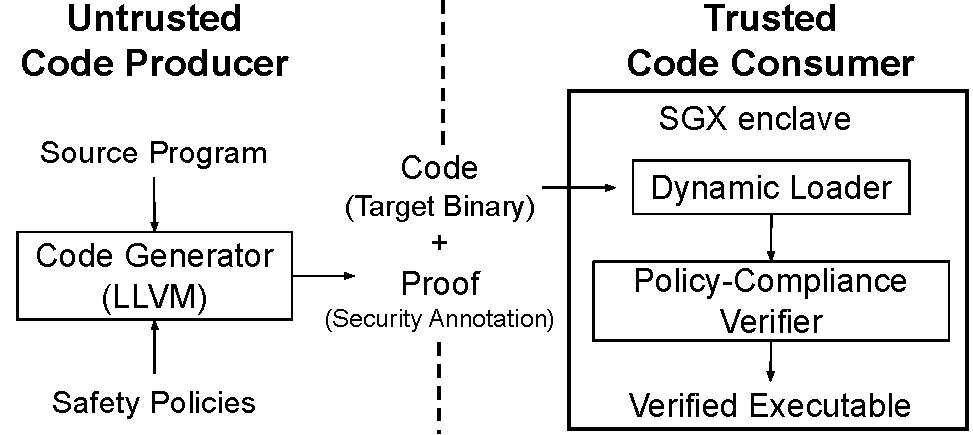
\includegraphics[scale=0.45]{figures/arch_overview.pdf}}
\centerline{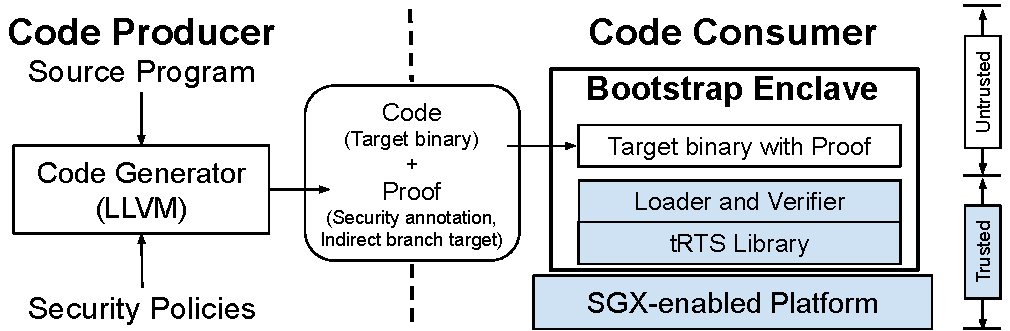
\includegraphics[scale=0.45]{figures/fg-bootstrap-layer.pdf}}
\caption{System overview}\label{fg-overview}
\vspace{-12pt}
\end{figure}

Instead, we construct a lightweight PCC-type scheme which includes an untrusted code producer and a trusted code consumer running in the bootstrap enclave (Fig.~\ref{fg-overview}). The overview design is derived from the original PCC idea while we have simplified it for our own purpose. The illustration of our design lists all components that are divided into two parts, trusted part and untrusted part. In our new PCC-based system, the proof is generated from the outside of the enclave during the compiling and can be verified at runtime inside. The inside verifier can cooperate with the outside compiler to make the verifier as lightweight as possible, using static verification of dynamic checks.
%\weijie{will unify them all into `verifier'}

In traditional PCC framework, the VCGen often exists as a compiler~\cite{colby2000certifying,leroy2006formal} or a sandbox~\cite{pirzadeh2010extended}, which is too heavy for limited executive resources. So here, we build our own lightweight PCC system to verify if a cloud service would leakage user’s data. Generally, we provide a code transformer for service code which needs to be verified, and a secure enclave for executing the verified service code. The only TCB in our design is the verifier code inside the enclave, including the dynamic-loader, the disassembler/rewriter (for rewritting structured guards), and the proof verifier (for checking verification hints). On the other hand, the whole trusted code consumer can be remotely attested (in Subsection~\ref{subsec-dynamicloader}), which can indirectly protect the integrity of for code provider, as well as the isolate valuable implementation detail from be accessed.

As mentioned above, to facilitate PCC framework working well in SGX and to make PCC more efficient, specifically to reduce the size of code consumer side, we move as much proof generation workload as possible to the code producer side, and leave as few verification workload as possible to the inside of the enclave.

\begin{figure*}[htbp]
\centerline{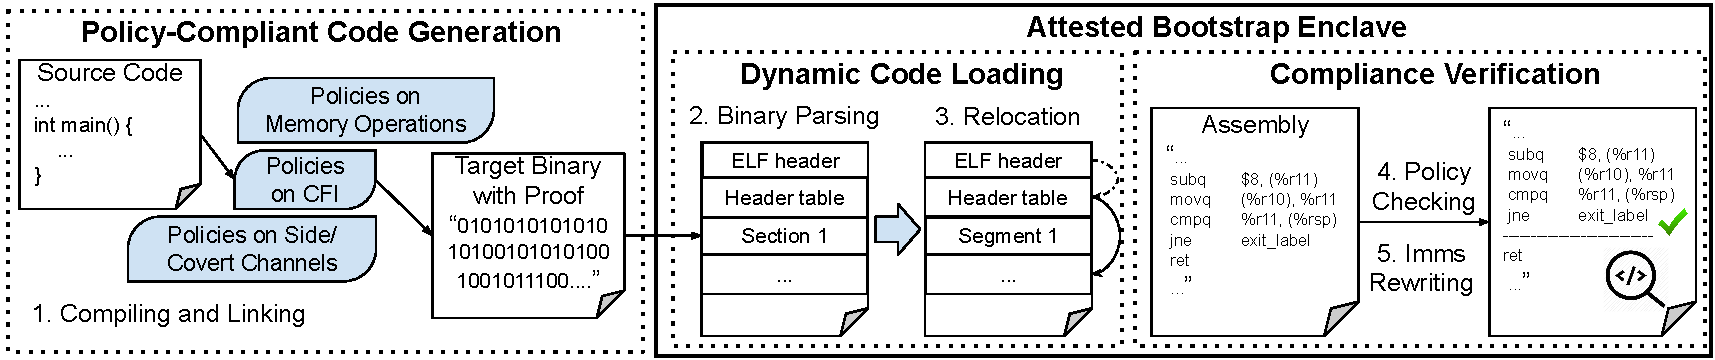
\includegraphics[scale=0.5]{figures/fg-workflow.pdf}}
\caption{Detailed framework and workflow}\label{fg-workflow}
%\wenhao{Typo: Attestated Bootstrap Enclave}
%\weijie{done. Thanks!}
\vspace{-15pt}
\end{figure*}
%\weijie{need some changes on the figure}

\vspace{3pt}\noindent\textbf{Workflow.} The workflow of our privacy-preserving TEE and PCC framework is shown as Figure~\ref{fg-workflow}. Unlike the typical interaction between the producer and consumer, the workflow encompasses several steps. 

First, the service code (target program) is instrumented using our own `code + proof' generator - a customized LLVM-based compiler (step 1,2). Then on the code consumer side, the loader source code and the verifier source code are compiled with SGX SDK to build the bootstrap enclave binary (step 3). Our loader can load and unload code after initialization (step 4), followed by being remote attested (step 5). Moreover, the `code + proof' can be transferred to code consumer where SGX is deployed, waiting for being dynamic loaded and rebased into the enclave (step 6). After being loaded, the verifier will rewrite some key immediate operands (Imm) and finally transfer the execution to the target program (step 7). 

\vspace{3pt}\noindent\textbf{Dynamic Code Loading and Unloading.} \label{subsec-dynamicloader}
%To ensure the bootstrap enclave's code can be completely public and can be attested, we propose a multi-step loader that can load and unload a generated `code + proof' dynamically. Unlike previous work, our proposed solution can resolve the problem that remote attestation conflicts with the dynamic relocation requirement~\cite{seo2017sgx}. Specifically, remote attestation requires code, data and security properties of the enclave to remain unchanged, while executing a private binary code needs relocation for execution, which is a modification to memory distribution. 
%Our proposal is based on the fact that binary code to be verified can not be trusted, so the measurement of the enclave should not include the untrusted code. Therefore, the code to be verified should be dynamically loaded and relocated after the bootstrap enclave is initiated. 
%\weijie{elaborates it later in Section Implementation}
%\vspace{3pt}\noindent\textbf{Separated Linking and Rebasing.} 
In our design, the linking procedures (linking and rebasing) of a target program are separated into both inside and outside the enclave respectively. SGX only accepts that code running inside an enclave is linked against the SGX SDK at build time. For a self-contained function (i.e., one does not use external elements), compiling and sending the bytes of the assembled code is enough. However, if the function uses external elements, a distributed mechanism is needed to map these elements into their corresponding positions at the enclave side. So we use separated linking and rebasing to assemble all the symbols of the entire code (including necessary libraries and dependencies) into one relocatable file (aka. linking), and then parse the symbols and load/relocate the code at runtime inside the enclave (aka. rebasing). Further, during the linkage procedure, we also load and relocate an indirect branch target entry list as part of the proof for later runtime verification.
%Note that legal jump addresses can not be settled until the rebasing procedure is completed because rebasing will modify the addresses of symbols.

The rebasing process starts with the bootstrap enclave receiving the generated binary code through a buffer. The dynamic loader's primary task is to rebase all of its symbols according to information in its relocation table. Therefore, the loader reads relocation tables in the code, updates symbol offsets in symbol tables, and loads symbols to addresses designated in relocation tables. After rebasing, the detailed memory layout is shown on the right side in Fig.~\ref{fg-dynloader}.




%\wenhao{can elaborate on this. The numbers are not in any order}

\subsection{Security Policies}\label{subsec-policies}
%\subsection{Security Policies for the Privacy Preserving Online Data Processing Scenario}\label{subsec-policies}

%Our general goal of defining safety policies is to design a Privacy-preserving TEE prototype on a service-oriented environment for data owner. Here, we make some rules to constrain our design.
In this scenario, the bootstrap enclave needs to enforce that the data will not be leaked by the untrusted service code, which is not exposed to the data provider. It can be achieved by enforcing several policies as follows. Notably, the policies put some constraints on the service code, yet we make a lot of effort on these constraints to ensure that the code functionality are intact and necessary for the CAT model.

\vspace{3pt}\noindent\textbf {Constraining Ecalls/Ocalls}. In such service-oriented scenarios, all the bridge functions should be public and attestable for normal use, we should make restrictions on them. The output is to be produced encrypted and the loader must deal with system calls via a trusted Ocall routine. All ECalls/OCalls will be audited and configured correctly by the bootstrap enclave.  

\vspace{2pt}\noindent$\bullet$\textit{ P0: Standard and Encrypted Output via legitimate Ocalls}. After the Remote Attestation and the session key exchange, messages sent from the enclave should be all encrypted. And for security consideration, they could be the same length to prevent further inference attacks.

\vspace{3pt}\noindent\textbf {Verifying Memory Operations}. In order to prevent data leakage during it being processed by a untrusted code provider, we need a verifier to check if this program is prone to write sensitive information from inside enclave to the outside world. 

\vspace{2pt}\noindent$\bullet$\textit{ P1: Preventing explicit memory stores to the outside of the enclave}. An enclave has the ability to write data outside of its EPC memory region arbitrarily. Therefore, the major policy is to prevent the untrusted code from copying the data across enclave boundaries. The policy-compliance verifier needs to ensure that the destinations of memory store instructions such as \texttt{MOV} are within the enclave address range (also known as the \texttt{ELRANGE}). %The first thing we should guarantee is no writes onto non-data section. In addition to check various memory write operations caused by instructions like MOV, we need to prevent another register save/spill operations that possibly push some register value to memory space.

\vspace{2pt}\noindent$\bullet$\textit{ P2: Preventing implicit memory stores to the outside of the enclave}. Illicit RSP register save/spill operations can do the trick of leaking sensitive information to memory via pushing a register value to an address specified by the stack pointer. 
    %To address this issue, stack operating instructions need be inspected so that the stack pointer never points to memory regions outside the enclave. 

\vspace{2pt}\noindent$\bullet$\textit{ P3: Preventing tampering of security-critical data within the bootstrap enclave}. This ensures that the code never reads or writes secrets in the SSA/TCS area, which is necessary because strong security properties no longer hold if the thread control structure data is used. In this case the verifier needs to ensure that the untrusted code does not tamper with this kind of data structure.
    %\item \textit{P4: does not read from or write to L’s memory}. %\weijie{User's private code does not load from L’s memory. } %\wenhao{auditing memory loads is heavy? We may need to argue the leakage is controlled?}

\vspace{3pt}\noindent\textbf{Constraining Control Transfers}. 
%In order to prevent attackers from bypassing our checks, we need do CFI checks on multiple aspects.\todo{on this part}
In our PCC-type scheme, the policy-compliance verifier performs static analysis of the untrusted code. It is essential to prevent attackers from dynamically redirecting the control flow at runtime, which may bypass the check performed when the code is initially loaded. In this respect, the following policies need to be enforced. 

\vspace{2pt}\noindent$\bullet$\textit{ P4: Data execution prevention for the RWX region}. In the currently SGX platforms that support only SGXv1 instructions, the untrusted code are loaded to pages with \texttt{RWX} properties. A software DEP scheme is needed to prevent the untrusted code from changing the code at runtime.

\vspace{2pt}\noindent$\bullet$\textit{ P5: Indirect branches shall not point to destinations that violate policies P1 to P4}. Such control flow integrity definitely should be guaranteed since the loaded code could be malicious so that it could bypass the mentioned policies. Therefore, this enforcement should be performed for all indirect control transfer instructions, including indirect calls, indirect jumps, and return instructions.
    %\item \textit{P6: Checking if control transfer targets are embedded in proof instrumentations}. If an attacker knows the details of the representation of proof (aka. those instrumentations inserted by our LLVM), he/she can exploit it and further sabotage the control flow.

\vspace{3pt}\noindent\textbf{Detecting leakage through AEX based side channels}. Side channels are difficult to eliminate and are severe threats to TEEs such as SGX. As shown in previous works, the abnormal AEXs can be used to detect many low-noise side channels within SGX, such as controlled channel attacks~\cite{xu2015controlled}, and same core L1/L2 cache attacks~\cite{chen2018racing}. We are not meant to design new side channel defenses, nevertheless we propose to transplant 
existing side channel detecting techniques, 
which illustrates the generality of the CAT model. 

%Side and covert channels often hide in the normal behaviors during program execution since the logic of service provider’s code would be very complicated. However, side channel prevention is not an easy task. Here we design some alternative policies for side channel mitigation.

\vspace{2pt}\noindent$\bullet$\textit{ Alternative P6: Detecting page faults with TSX support}. 

\vspace{2pt}\noindent$\bullet$\textit{ Alternative P7: Detecting AEX by monitoring the SSA}.

\vspace{3pt}\noindent\textbf{Multi-Usesr Isolation}. When protecting in-enclave time-sharing services, a big challenge is to prevent the service program infected by one user from victimizing another user, and the confidentiality of a user’s data left in the enclave to protect it from leaking to the subsequent user receiving the service.

\vspace{2pt}\noindent$\bullet$\textit{ P8: User data cleansing}. The purpose of the data cleansing and the exit sanitization is to reset the service state and clean up the old user’s data right after execution is done. Except the persistent data of the user, all other data will be cleaned up, together with the content of SSA and registers.

\subsection{Policy-Compliant Code Generation}
\label{subsec-producer}
In this section we present the design of the code generator, which given the source program can produce binary code that enforces the policies P1 to P5, and can be easily verified. The design of the policy verifier will be presented in Sec.~\ref{subsec:verify}. Since we do the verification at the assembly level and the target binary loaded in the bootstrap enclave will finally be disassembled, the code generator does not need to be trusted.

%When the target binary wants a syscall or the in-enclave service ends, the computing results need to be output in a standard format.
\vspace{3pt}\noindent\textbf{Enforcing P0}. The output message for the in-enclave service is encrypted using session key after RA. Before that, to construct the output message, the plaintext is padded to a constant length if have to. Meanwhile, the output functions are wrapped by our customized Ocall stubs. On the other hand, 37 common system calls are also wrapped with Ocall stubs for possible system interactions.\wenhao{we need to discuss: admitting arbitrary ocalls could lead to information leakage by ocall patterns}

%enforcing mem ops
\vspace{3pt}\noindent\textbf{Enforcing P1}. The generator instruments all storing instructions to check if they are writing to the memory out of the enclave. The code consumer inside the enclave confirms such security check instructions are in place.

\vspace{3pt}\noindent\textbf{Enforcing P2}. The generator prevents implicit memory write crossing the enclave boundaries by making sure the stack pointer never point to memory regions outside the enclave. It locates all the instructions modifying the stack pointer explicitly, and inserts instructions to check the validity of the stack pointer after them. The code consumer confirms the placement of these check instruction. Furthermore, the code consumer prevents implicit modification of the stack pointer by adding guard pages (i.e., pages granted no permissions) around the stack boundaries. 

\vspace{3pt}\noindent\textbf{Enforcing P3}. Similar to enforcing P1 and P2, the code generator further enforces that (both explicit and implicit) memory write operations cannot alter the security-critical data once the untrusted code is loaded and verified. These check instructions are verified by the code consumer inside the enclave. 

%enforcing CFI
\vspace{3pt}\noindent\textbf{Enforcing P4}. Similar to enforcing P1 and P2, the code generator and consumer enforce that (both explicit and implicit) memory write operations cannot modify the \texttt{RWX} pages.

\vspace{3pt}\noindent\textbf{Enforcing P5}. For indirect calls or indirect jumps, the code generator firstly extract all legal destination addresses of them. Theses addresses are stored in a specific data region. Then it instruments code to check the targets of all the indirect call/jump instructions in the code to ensure they only direct to addresses listed in the data region. These instruments can be efficiently verified by the in-enclave code consumer.

%enforcing side channel mitigations
\vspace{3pt}\noindent\textbf{Enforcing P6}.
We enforce P6 by introducing the idea of T-SGX~\cite{shih2017t}. As a compiler-level scheme that automatically transforms a normal enclave program into a secured one, T-SGX can isolate the fallback handler and other transaction control code, called springboard, from the original program’s code and data pages to ensure that exceptions including page faults and timer interrupts can only be triggered on the springboard. We take advantage of it and implement instruction wrappers that encompass all boundaries between any basic blocks and branches. The fallback route of the TSX wrapper records the number of transaction aborts, which ensures that if a threshold is exceeded, the program is forced to exit. 

\vspace{3pt}\noindent\textbf{Enforcing P7}.
We enforce P7 by retrofitting Hyperrace~\cite{chen2018racing}. However, unlike Hyperrace doing the physical-core co-location tests, here we only monitor how often the interrupts/AEXs happen. L1/L2 cache-based channel can be detected when certain number or more interrupts/AEXs occur in one basic block or every k instructions.

%enforcing multi-user isolation
\vspace{3pt}\noindent\textbf{Enforcing P8}. Before the bootstrap enclave is destroyed, all user data is cleared after the execution transferred back to the loader.

\subsection{Compliance Verification}
\label{subsec:verify}

Due to the thorough generated proof with compliance, the bootstrap enclave can quickly verify the validity of the proof, and it can compare the conclusions of the proof to its own security policy to determine whether the application is safe to execute.

\vspace{3pt}\noindent\textbf{Just-enough Disassembling.} Accurate and complete binary disassembly is a difficult problem in general due to indirect control flow transfers. We built a lightweight disassembler with the assistance of the compiler outside the enclave. Our disassembler starts with the program entry and follows the program control flow. When we encounter indirect control flow transfers such as indirect jumps and indirect calls, we use the valid target list provided by the compiler to find the targets of indirect control flows. Note that our verifier will ensure that there are runtime checks before every indirect control flow, which guarantees that the actual control flow targets are inside the list provided by the compiler. In this way, the untrusted compiler is not able to hide dangerous transfer targets by omitting them in the list. The runtime check ensures the integrity of the target list provided by the compiler.
}
\section{Implementation}\label{sec-implementation}

We implemented the prototype on Linux/x86 arch. Specifically, we implemented the code generator with LLVM 9.0.0, and built other parts on an SGX environment.
The LLVM passes consist of several types of instrumentations for the code generator. 
Besides, we implemented the bootstrap enclave based on Capstone~\cite{capstone} as the disassembler. 

%from scratch and made a best effort to reduce the size of the trusted computing base, where consists of about 1900 lines of code in total.
%Yet the loader we implemented is very small that only consists of less than 400 lines of C code, while the verifier consists of less than 500 lines that is made from scratch.

%\wenhao{stack guard page}\weijie{add it in the following subsection}

%\subsection{Assembly-level Instrumentation}\label{subsec-instrument}
\subsection{Multi-level Instrumentation}\label{subsec-instrument}

%\xiaofeng{To support flexible control of code to comply with different security policies, we implanted a set of switches into our code generator. These switches work on the IR level and their on/off states can be passed down to the target code level for further control, depending on the policies to be enforced. In this way, we separate  This \textit{separating mechanism and policy} design and implementation can make our frame more scalable and flexible for various security policies. }


\begin{figure}[htbp]
\centerline{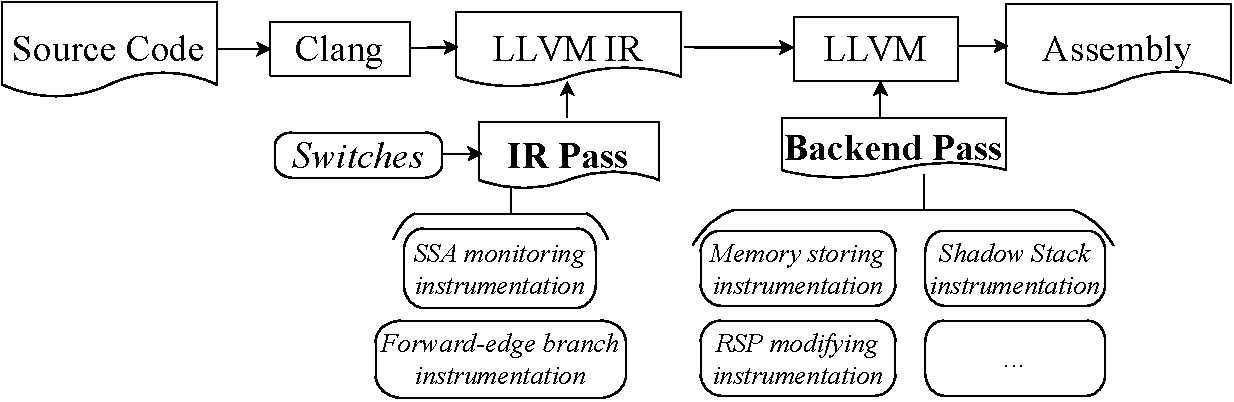
\includegraphics[scale=0.42]{figures/fg-codegen.pdf}}
\caption{ Workflow of flexible code generation}\label{fg-codegen}
%\wenhao{please update Hyperrace to SSA monitoring}
\vspace{-8pt}
\end{figure}

The code generator we built is mainly based on LLVM (Fig.~\ref{fg-codegen}), and the assembly-level instrumentation is the core module. To address the challenge of limited computing resources described in Section~\ref{challenge-tcb}, this code generator tool is designed and implemented comprehensively, to make the policy verifier small and exquisite. More specifically, we implemented modules for checking memory writing instructions, RSP modification, indirect branches and for building shadow stack. And we reformed an instrumentation module to generate side-channel-resilient annotations. 
To support flexible control of code to comply with different security policies, we implanted a set of switches into our code generator. These switches work on the IR level and their on/off states can be passed down to the target code level for further control, depending on the policies to be enforced. This \textit{separating mechanism and policy} design makes that we can not only demonstrate the security policies for several real-world scenarios, modules of the annotation generation for customized functionalities can also be integrated into the code generator.
 

Here is an example (Figure~\ref{fg-mov}). The main function of the module for checking explicit memory write instructions (P1) is to insert annotations before them. Suppose there is such a memory write instruction in the target program, `\texttt{mov reg, [reg+imm]}',
the structured annotation first sets the upper and lower bounds as two temporary Imms (0x3ffffffffffff and 0x4ffffffffffff), and then compares the address of the destination operand with the bounds. The real upper/lower bounds of the memory write instruction are specified by the loader later. If our instrumentation finds the memory write instruction trying to write data to illegal space, it will cause the program to exit at runtime. 
%\revise{The code snippet (structured format of the annotation) is shown in Figure~\ref{fg-mov}.}

%\weijie{more explanation here with Hoare logic}


%\revise{The code snippet (structured format of the annotation) is shown in Figure~\ref{fg-mov}. 
%\weijie{more explanation here with Hoare logic}}
%More details can be found at Appendix~\ref{appendix-instrumentation}.

\begin{figure}
\begin{center}
\begin{minipage}{0.4\textwidth}
%[basicstyle=\scriptsize,numbers=left, numberstyle=\scriptsize,,keywordstyle=\color{blue!70},commentstyle=\color{red!50!green!50!blue!50}, rulesepcolor=\color{red!20!green!20!blue!20}]
\begin{lstlisting}[basicstyle=\scriptsize]
pushq   %rbx    ;save execution status
pushq   %rax
leaq    [reg+imm], %rax ;load the operand
movq    $0x3FFFFFFFFFFFFFFF, %rbx  ;set bounds
cmpq    %rbx, %rax
ja      exit_label
movq    $0x4FFFFFFFFFFFFFFF, %rbx  ;set bounds
cmpq    %rbx, %rax              
jb      exit_label
popq    %rax
popq    %rbx
movq    reg, [reg+imm]
\end{lstlisting}
\end{minipage}
\end{center}
\vspace{-8pt}
\caption{Store instruction instrumentation}\label{fg-mov}
\vspace{-15pt}
\end{figure}

%Although using the code generator we could automatically produce an instrumented object file, we still need to deal with some issues manually that may affect practical usage. As the workflow described in Figure~\ref{fg-workflow}, the first job to make use of CAT system is preparing the target binary.  Service-specific libraries and some dependencies also should be built and linked against the target program (detailed in Appendix~\ref{appendix-preparing}).
%Nevertheless, we have to do some preparing work before the target program loading~\ref{appendix-preparing}.

\subsection{Building Bootstrap Enclave}\label{subsec:bootstrap-impl}
%\begin{figure}[htbp]
\centerline{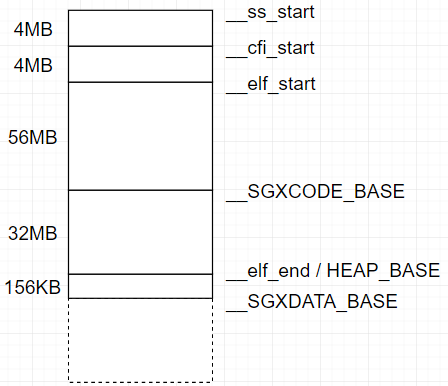
\includegraphics[scale=0.42]{figures/memlayout.png}}
\caption{Memory Layout}\label{fg-memlayout}
\label{fig}
\end{figure}
%\vspace{3pt}\noindent\textbf{Reserving Blank Memory Space.}
Following the design in Section~\ref{subsec:verify}, we implemented a \textit{Dynamic Loading after RA mechanism} for the bootstrap enclave. The enclave is initiated based upon a configuration file (a.k.a. the manifest file), which specifies the system calls the enclave is allowed to make in compliance with security policies, the protection enforced through instrumented OCall stubs. During the whole service, the data owner can only see the attestation messages related to the bootstrap's enclave quote, but learn nothing about service provider’s code.

%\xiaofeng{Just like Graphene-SGX~\cite{} and Occlum~\cite{}, our approach necessary OCalls for enforcing P0 can be prescribed with a configuration file.}

\begin{figure}[htbp]
\centerline{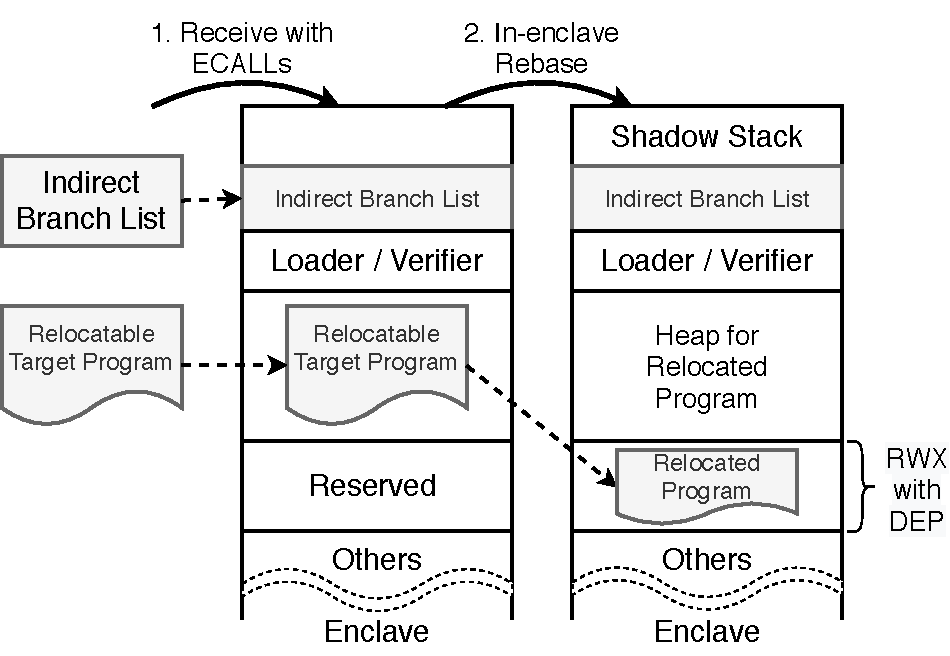
\includegraphics[scale=0.45]{figures/fg-dynloader.pdf}}
\caption{Detailed workflow of the dynamic loader}\label{fg-dynloader}
\vspace{-10pt}
\end{figure}

\vspace{3pt}\noindent\textbf{Remote attestation}.\label{subsec:ra-impl}
Once the bootstrap enclave is initiated, it needs to be attested. 
\revise{We leverage the RA-TLS routine}~\cite{knauth2018integrating} and adjust it to our implementation.
%We leverage the original RA routine~\cite{originalra} and adjust it to our design. 
%The original RA routine requires that the host, which is assumed to run the enclave as the `client', initiates the attestation towards the `server', who owns the data. While in this CCaaS scenario, the service runs in the enclave while the remote user owns the data. So, we modify this routine to enable a remote CCaaS user to initiate the attestation.
The RA procedures are invoked inside the bootstrap enclave after secret provision between parties. After obtaining a quote of the bootstrap enclave, the remote data owner submit the quote to IAS and obtain an attestation report. 
%This report is signed by the IAS report signing private key, which can be validated by the data owner.

%\xinyu{I think the following paragraph is slightly misleading because in my implementation, RA is actually initiated by the remote user. The reason why RA should be invoked by user is stated in the first paragraph of the Remote Attestation part.}
%Using our customized Remote Attestation flow, service provider’s enclave can be attested right after enclave initialization. Since the loader/verifier code is public, the RA procedures can be invoked by simply calling \verb|sgx_ra_init()| inside the service provider’s enclave after secret provision between the remote user and the service provider. After obtaining an enclave quote of the current running enclave which is signed with the platform's EPID key, the remote data owner can submit the quote to IAS and obtain an attestation report. This report is signed by the IAS Report Signing private key, and the remote user can validate this signature using the IAS Report Signing Public Key.


\vspace{3pt}\noindent\textbf{Dynamic loader}. 
When the RA is finished, the trust between data owner and the bootstrap enclave is established. Then the user can locally/remotely call Ecall (\verb|ecall_receive_binary|) to load the service binary instrumented with security annotations and the indirect branch list without knowing the code. 
User data is loaded from untrusted memory into the trusted enclave memory when the user remotely calls Ecall (\verb|ecall_receive_userdata|), to copy the data to the section reserved for it.

% \revise{Just like Graphene-SGX~\cite{} and Occlum~\cite{}, necessary OCalls for enforcing P0 can be prescribed with a configuration file.}

Then, the dynamic loader in the bootstrap enclave loads and relocates the generated code. 
The indirect branch list, which is comprised of symbol names that will be checked in indirect branch instrumentations, will be resolved at the very beginning. 
%Those symbol names will be replaced with the value of addresses, i.e., their actual addresses in the enclave memory space. %\xinyu{actually in our implementation, ECALL ecall\_receive\_entrylabel is first called before ecall\_receive\_binary} %The dynamic loading procedure is invoked when the user remotely calls ECALL (\verb|ecall_receive_entrylabel|). 
Our implementation  utilizes 4M memory (by default) space for storing indirect branch targets, and for operating a shadow stack.
We further reserve more memory space for hosting the uploaded binary and data, which can be configured in the manifest file.
%The heap base address is slightly larger than the end of received binary.
%, and 0x27000 Bytes (156 KB) space is reserved for the loader's own heap. 
After relocation, the detailed memory layout and some key steps are shown in Figure~\ref{fg-dynloader}. %\revise{We implement both software-based and SGXv2-based DEP protections.}



%\revise{And we reserve more than 32M memory space for received binary and for `.data' section, which also can be configured in the manifest file.}

\vspace{3pt}\noindent\textbf{Policy verifier}.\label{subsec-boundarychecking}
The policy-compliance verifier, is composed with three components - a clipped disassembler, a verifier, and an immediate operand rewritter.

\vspace{2pt}\noindent$\bullet$\textit{ Clipped disassembler.} 
We enforce each policy at assembly level. 
Thus, we incorporate a lightweight disassembler inside the enclave. To implement it, we remove unused components of this existing wide-used framework, and use Recursive Descent Disassembly to traverse the code. Also, we use the \textit{diet} mode, making the engine size at least 40\% smaller~\cite{quynh2014capstone}. 

\vspace{2pt}\noindent$\bullet$\textit{ Policy verifier.}\label{subsec-policyverifer}
The verifier and the following rewriter do the work just right after the target binary is disassembled, according the structured guard formats provided by our code generator. The verifier uses a simple scanning algorithm to ensure the policies applied in assembly language instrumentation. 
%Then, the verifier's job is done and the proof (instrumentations) will do the magic - checking policies. 
Specifically, the verifier scans the whole assembly recursively along with the disassembler. It follows the clipped disassembler to scan instrumentations before/after certain instructions are in place, and checks if there is any branch target pointing between instructions in those instrumentations.
%Moreover, legal jump addresses can be obtained from symbol tables by searching indirect branch target names.

\vspace{2pt}\noindent$\bullet$\textit{ Imm rewriter.}\label{subsec:immrewriter} One last but not least step before executing the target binary code is to resolve and replace the Imm operands in instrumentations, including the base of the shadow stack, and the addresses of indirect branch targets (i.e. legal jump addresses). For example, the genuine base address of shadow stack is the start address \verb|__ss_start| of the memory space reserved by the bootstrap enclave for the shadow stack. And the ranges are determined using functions of Intel SGX SDK during dynamic loading (Section~\ref{subsec:verify}).
%With unknown addresses replaced to corresponding addresses in the enclave memory (by the Imm rewriter in Subsec.~\ref{subsec:immrewriter}), the binary code is prepared for privacy policy compliance verification.
%We use the simplest way to rewrite Imm operands.
Table~\ref{tb-rewritter} shows what the specific values should be before and after rewriting, respectively. 
%\weijie{talk about those vars} 
The first column of table~\ref{tb-rewritter} shows the target we need to rewrite while loading. For instance, the upper bound address of data section would be decided during loading, but it would be 0x3ffffffffffffffff (shown in the 2nd. column) during the proof generation and will be modified to the real upper data bound address. The third column shows the variable name used in our prototype.
%how we get those bounds, through sgx sdk functions

\begin{table}[htbp]
\footnotesize
\caption{Fields to be rewritten}\label{tb-rewritter}
\vspace{-5pt}
\begin{center}
\begin{tabular}{|c|c|c|}
\hline
\textbf{Target imm description} & \textbf{From} (hex) & \textbf{To} \\
\hline
Upper bound of .data & 3ffffffffffffffff & \verb|upper_data_bound| \\
\hline
Lower bound of .data & 4ffffffffffffffff & \verb|lower_data_bound| \\
\hline
Upper bound of stack & 5ffffffffffffffff & \verb|upper_stack_bound| \\
\hline
Lower bound of stack & 6ffffffffffffffff & \verb|lower_stack_bound| \\
\hline
Upper bound of .code & 7ffffffffffffffff & \verb|lower_code_bound| \\
\hline
Lower bound of .code & 8ffffffffffffffff & \verb|lower_code_bound| \\
\hline
\# of indirect branch targets & 1ffffffff & \verb|branch_target_idx| \\
\hline
Addr. of branch target list & 1ffffffffffffffff & \verb|__branch_target| \\
\hline
Addr. of the shadow stack & 2ffffffffffffffff & \verb|__ss_start| \\
\hline
\end{tabular}
\end{center}
\vspace{-15pt}
\end{table}

\section{Analysis and Evaluation}\label{sec-evaluation}
%In this section we report our security analysis and performance evaluation of CAT-SGX.
%In this section, we evaluate our proposal, to see how much the TCB of our system is and each security guarantee that offered by our design, and we show how much additional overhead our CAT-SGX system would cause. 

\subsection{Security Analysis}\label{subsec-securityanalysis}

\noindent\textbf{TCB analysis}. 
The hardware TCB of \textsc{Deflection} includes the TEE-enabled platform, i.e. the SGX hardware. The software TCB includes the components shown in Table~\ref{tb-tcb}. Security and privacy are guaranteed by the lightweight in-enclave verifier (in TCB), even if the code generator has mis-compilation errors. The correctness of our verifier can be formally verified, using memory safety verification tools such as SMACK and model checking tools such as SPIN.

The loader we implemented consists of less than 600 lines of code (LoCs) and the verifier includes less than 700 LoCs, also integrating the SGX SDK and part of Capstone libraries. 
The binary sizes of shielded runtimes such as Graphene-SGX increase to 2.5 times or more compared to ours. Currently, Occlum has not integrated the SFI feature in its latest version~\cite{occlum}, thus we can only know the lower bound of its TCB size.
Altogether, our software TCB contains a self-contained enclave binary (1.9 MB) with a shim libc (2.6 MB). By comparison, most solutions are at least an order of magnitude larger as compared to \textsc{Deflection}.

%\wenhao{I think wed better have a table to show all tcb components: categories: SGX SDK/loader/disassembler+rewriter/enforcing policies/}
%According to the threat model~\ref{subsec-threat}, besides the Intel's trusted library - tRTS and the SGX Driver, the software part of the TCB includes the bootstrap enclave software. The SGX hardware, as a TEE-enabled platform, is also part of our TCB on the hardware side. The bootstrap enclave implementation (Section~\ref{subsec:bootstrap-impl}) consists of the loader and the verifier, the wrapped ECall/OCall interfaces, and a simple realization of RA.


\begin{table}[htbp]
\footnotesize
\caption{TCB comparison with other solutions}\label{tb-tcb}
\vspace{-8pt}
\begin{center}
\begin{tabular}{|c|c|c|c|}
\hline
\textbf{Shielding runtimes} & \textbf{Core components} & kLoCs & \textbf{Size(MB)} \\
\hline
 & Eglibc & 892 & \\
Ryoan & NaCl sandbox & 216 & $>$ 19 \\
 & Naclports & 460 & \\
\hline
SCONE & OS Shield and shim libc & 187 & $>$ 16 \\
\hline
 & Glibc & 1200 & \\
Graphene-SGX & LibPAL & 22 & $>$ 58.5 \\
 & Graphene LibOS & 34 & \\
\hline
 & Occlum shim libc & 93 & \\
Occlum & Verifier & N/A & $>$ 8.6 \\
%1.7+2.5+3.1+1.3
 & Occlum LibOS and PAL & 24.5 & \\
\hline
 & Interface and libc & 65  & \\
\textsc{Deflection} & Loader/Verifier & 1.3 & 3.5 \\ 
 & RA/Encryption & 0.2 & \\
\hline
\end{tabular}
\end{center}
%*  Ryoan reports a TCB of multiple modules (including at least a NaCl sandbox), however we do not have the access to the system for comparison.
%* Occlum leverages Rust SGX SDK instead of solely using Intel SGX SDK which is used by other solutions.
\vspace{-10pt}
\end{table}







%%%%----------------------------------------------------------------%%%%
\ignore{

\weijie{comparison}
%\xiaofeng{


\vspace{2pt}\noindent$\bullet$\textit{ Loader and verifier}.
The loader we implemented consists of
%While the main function of dynamic loading we implemented is very small that only consists of 
less than 600 lines of code (LoCs) and the verifier includes less than 700 LoCs, also integrating the SGX SDK and part of Capstone libraries. 
%Yet the whole loader and verifier is supported by the Capstone and an ELF parser so that part of the \verb|libcapstone.a| and the \verb|libelf.a| should also be included.

\vspace{2pt}\noindent$\bullet$\textit{ ECall/OCall stubs for supporting P0}. This was implemented in less than 500 LoCs. 
%Components to process the input/output and its configuration brings in less than 500 lines.

\vspace{2pt}\noindent$\bullet$\textit{ Simple RA protocol implementation}. The implementation  (Section~\ref{subsec:ra-impl}) is done with about about 200 LoCs.

%\vspace{2pt}\noindent$\bullet$\textit{ Dependencies}. Our framework is built upon several existing libraries, which include the SGX SDK libraries, parts of Capstone libraries, and an ELF parser.
\noindent Altogether, our software TCB contains less than 2000 LoCs and some dependencies, which was compiled into a self-contained binary with 1.9 MB in total. By comparison, XXX includes XXX LoCs, XXX in binary in its TCB, based upon our analysis of its code~\cite{shinde2017panoply}. 
%}
%\weijie{openssl}

}







\ignore{
The loader we implemented consists of
%While the main function of dynamic loading we implemented is very small that only consists of 
less than 600 lines of code (LoCs) and the verifier includes less than 700 LoCs, which also integrates SGX SDK and part of Capstone libraries. 
%Yet the whole loader and verifier is supported by the Capstone and an ELF parser so that part of the \verb|libcapstone.a| and the \verb|libelf.a| should also be included.

\vspace{2pt}\noindent$\bullet$\textit{ ECall/OCall stubs for supporting P0}. This was implemented in less than 500 LoCs. 
%Components to process the input/output and its configuration brings in less than 500 lines.

\vspace{2pt}\noindent$\bullet$\textit{ Simple RA protocol realization}. The implementation  (Section~\ref{subsec:ra-impl}) introduces about 200 LoCs.

%\vspace{2pt}\noindent$\bullet$\textit{ Dependencies}. Our framework is built upon several existing libraries, which include the SGX SDK libraries, parts of Capstone libraries, and an ELF parser.
\noindent Altogether, our software TCB contains less than 2000 LoCs and some dependencies, which was compiled into a self-contained binary with 1.9 MB in total.
\weijie{openssl}
}

\vspace{3pt}\noindent\textbf{Policy analysis}. 
Here we show how the policies on the untrusted code, once enforced, prevent information leaks from the enclaves. In addition to side channels, there are two possible ways for a data operation to go across the enclave boundaries:
%Path to the outside of an Enclave includes only two aspects - 
bridge functions~\cite{van2019tale} and memory write.

\vspace{2pt}\noindent$\bullet$\textit{ Bridge functions}. 
With the enforcement of P0, the loaded code can only invoke our OCall stubs, which prevents the leak of plaintext data through encryption and controls the amount of information that can be sent out.
%(to the code provider in CDaaS).
%. With the ECall/OCalls which are to process input/output messages will not reach the plain-text data directly.

\vspace{2pt}\noindent$\bullet$\textit{ Memory write operations}. All memory writes, both direct memory store and indirect register spill, are detected and blocked. Additionally, software DEP is deployed so the code cannot change itself.  Also the control-flow integrity (CFI) policy, P5, prevents the attacker from bypassing the checker with carefully constructed gadgets by limiting the control flow to only legitimate target addresses. 
%since CFI policies are enforced.

As such, possible ways of information leak to the outside of the enclave are controlled. As proved by previous work~\cite{sinha2015moat,sinha2016design} the above-mentioned policies (P1-P5) guarantee the property of confidentiality. Furthermore the policy (P5) of \textit{protecting return addresses and indirect control flow transfer, together with preventing writes to outside} has been proved to be adequate to construct the confinement~\cite{schuster2015vc3,sinha2016design}. So, enforcement of the whole set of policies from P0 to P5 is sound and complete in preventing explicit information leaks. 
In the meantime, our current design is limited in side-channel protection. We can mitigate the threats of page-fault based attacks and exploits on L1/L2 cache once Hyper-threading is turned off or HyperRace~\cite{chen2018racing} is incorporated (P6). However, defeating the attacks without triggering interrupts, such as inference through LLC is left for future research.  



%\subsection{Use Cases and Leakage Control}\label{subsec:usecases}
%\weijie{we can close most covert channels via P0}


%Our security analysis (Section~\ref{subsec-securityanalysis}) has shown that CAT-SGX can prevent explicit data leak. Here we further demonstrates that even though CAT-SGX cannot eliminate the covert channel threat, it provides a level of privacy protection that existing shielding runtimes cannot achieve. 

%for page limit
\ignore{
\vspace{2pt}\noindent\textbf{Covert-channel mitigation}. Since the data owner is the recipient of an enclave's output, all a malicious enclave program can do is to signal to the untrusted OS the content of the data through covert channels, e.g., through system call interfaces. To address this type of covert channel leak, we can control the enclave program's input and output behaviors. One approach is to restrict it, making a single ECall for data input and a single OCall for result output. Consider that the time granularity of the attacker's observation is $R$ (e.g., second), and the time interval of the input/output pair is $T$. The amount of the information (in bit) the attacker can get out to the OS becomes $L_{et} = \log_2 {(T/R)}$. What our approach can do is to modulate this interval, e.g., fixing it to a maximum duration or rounding it to a multiple of a time unit like a minute, so as to control the leak.  Also, all outputs from the enclave are padded to the same size, to avoid the leak through packet length.
}

%As mentioned earlier, covert channels can also be built through SGX hardware, such as cache, memory management, etc. CAT-SGX mitigates such threats through enforcement of P6. 
With such protection, still our design cannot eliminate all covert channels, which is known to be hard. However, it is important to note that other SGX runtimes, including SCONE, Graphene-SGX, Occlum, provide no such protection either. An exception is Ryoan, which pads its enclave output to the same size, as we do. However, it does not handle the leak from the hardware-based channels.

%Besides, side channel induced by shared hardware can also contribute to some data leak, yet novel transient side channel attacks may leak a few bits~\cite{canella2019systematic}, which can be mitigated via P6 or more alternative policies.





%\noindent\textbf{HTTPS server}. We further looked into another realistic and more complicated case.


%\weijie{Image processing. Image classification as a service is an emerging area.we consideredthat  a  batch  of  one  user’s  data  was  sent  for  processing,  withvarious batch sizes. }




\subsection{Performance Evaluation}\label{subsec-experiments}


\revise{
Here we discuss  performance overhead of different level protections \textsc{Deflection} can provide. These settings include just explicit memory write check (P1), both explicit memory write check and implicit stack write check (P1+P2), all memory write and indirect branch check (P1-P5), and together with side channel mitigation (P1-P6).}
%\weijie{need to modify all P7 to something else}
%\weijie{less narrative, more analysis}

%We evaluated the performance of our implementation on various settings. 


%now focus on the overhead evaluation. The benchmarks include various workloads. We quantify the time and space costs of our prototype by enforcing the execution of the described policies.
%\wenhao{talk about the goal for evaluation}


\noindent\textbf{Testbed setup}. 
%As same as the implementation, our evaluation was also completed on Linux/x86. 
In our research, we evaluated the performance of our prototype and tested its code generation and code execution. All experiments were conducted on Ubuntu 18.04 (Linux kernel version 4.4) with SGX SDK 2.5 installed on Intel Xeon CPU E3-1280 with 64GB memory.
%The maximum heap size and maximum stack size set by all enclaves during testing are 0x2000000 and 0x1800000, respectively. The version of SGX driver we use is 2.
%However, Intel has not shipped SGXv2 CPUs widely. So we evaluate the \textsc{Deflection} model on SGXv1 to show its compatibility.
Also we utilized  GCC 5.4 to build the bootstrap enclave and the SGX application, and the parameters `-fPIC', `-fno-asynchronous-unwind-tables', `-fno-addrsig', and `-mstackrealign' to generate x86 binaries. 

%for page limit
\ignore{
\begin{table}[htbp]
\footnotesize
\caption{Additional code size and execution time}\label{tb-simple-perf}
\vspace{-5pt}
\begin{center}
%\begin{tabular}{|c|c|c|c|c|c|c|c|c|c|}
\begin{tabular}{|c|cc|cc|}
\hline
%\textbf{Application Name} & \textbf{Size} & \textbf{Size (P1\textasciitilde P5)} & \textbf{Size (P1\textasciitilde P5+P6)} & \textbf{Size (P1\textasciitilde P5+P6-SSA)} & \textbf{Time} & \textbf{Time (P1\textasciitilde P5)} & \textbf{Time (P1\textasciitilde P5+P6)} & \textbf{Time (P1\textasciitilde P5+P6-SSA)}\\
%\textbf{Application Name} & \textbf{Size} & \textbf{Size (P1\textasciitilde P5)} & \textbf{Size (P1\textasciitilde P6)} & \textbf{Execution Time} & \textbf{Execution Time (P1\textasciitilde P5)} & \textbf{Execution Time (P1\textasciitilde P6)}\\
\textbf{Application} & \textbf{Size(P1-P5)} & \textbf{(P1-P6)} & \textbf{Time(P1-P5)} & \textbf{(P1-P6)}\\
%\hline
%bm\_hello.c & 3.6K & 1.218s \\
\hline
clock & +3.83\% & +4.31\% & +14.6\% & +15.8\% \\
\hline
malloc\_and\_magic & +4.41\% & +5.29\% & +14.4\%  & +22.0\% \\
\hline
malloc\_memalign & +4.80\% & +5.68\% & +14.8\% & +22.6\% \\
\hline
malloc\_and\_sort & +6.73\% & +8.17\% & +16.0\% & +27.6\% \\
\hline
memcpy & +68.1\% & +134\% & +2.97\% & +15.3\% \\
\hline
memchr & +59.6\% & +116\% & +3.39\% & +15.0\% \\
\hline
sprintf & +5.71\% & +8.57\% & +6.65\% & +18.2\% \\
\hline
sort\_and\_binsearch & +10.1\% & +14.6\% & +6.48\% & +18.3\%\\
\hline
Average & +\% & +\% & +\% & +\%\\
\hline 
\end{tabular}
\end{center}
\vspace{-8pt}
\end{table}



\vspace{3pt}\noindent\textbf{Performance on simple applications}. We used the applications provided by the SGX-Shield project~\cite{seo2017sgx} as a micro-benchmark. In our experiment, we ran each test case for 10 times, measured the resource consumption in each case and reported the median value. Specifically, we first set the baseline as the performance of an uninstrumented program running through a pure loader (a loader that only does the dynamic loading but no policy-compliance checking). Then we compared the baseline with the performance of instrumented programs to measure the overheads. Also the compilation time of each micro-benchmark varies from several seconds to tens of seconds, which is negligible compared with conventional PCC methods (2-5$\times$)~\cite{necula2001oracle}.
%measured the runtime overhead and  the baseline being an uninstrumented program running in a pure loader (a loader that only does the dynamic loading but no policy-compliance checking). Then we instrumented those programs and measure the execution time. The compilation time of each micro-benchmark varies from several seconds to tens of seconds, which is negligible compared with conventional PCC methods (2\textasciitilde 5$\times$)~\cite{necula2001oracle}.
%\wenhao{show how long PCC takes}
%on simple application bench
%geometry mean of performance overhead of P1~P5: 1.098
%geometry mean of performance overhead of P1~P6: 1.193
%geometry mean of storage overhead of P1~P5: 1.181
%geometry mean of storage overhead of P1~P6: 1.295

Table~\ref{tb-simple-perf} illustrates overheads of our approach. 
From the table, we can see that the size of instrumented binaries (a.k.a. the ``code + proof'') is 18.1\% larger than the original code and their executions were delayed by 9.8\% on average
when only P1-P5 are enforced. The overhead becomes 30\% in memory and 19\% in time when all policies, including P6, are enforced. Note that this batch of benchmarks are mostly a `first-simple-processing-then-syscall' program. At the worst case - `malloc\_and\_sort', \textsc{Deflection} showed 27.6\% overhead in execution time. 
}

\begin{table}[htbp]
\footnotesize
\caption{Performance overhead on nBench}\label{tb-nben-perf}
\vspace{-5pt}
\begin{center}
\begin{tabular}{|c|c|c|c|c|}
\hline
\textbf{Program Name} & \textbf{P1} & \textbf{P1+P2} & \textbf{P1-P5} & \textbf{P1-P6}\\
\hline
NUMERIC SORT  & +5.18\% & +6.05\% & +6.79\% & +12.0\% \\
\hline
STRING SORT  & +8.05\% & +10.2\% & +12.4\%  & +18.4\% \\
\hline
BITFIELD  & +6.11\% & +11.3\% & +15.5\% & +17.9\% \\
\hline
FP EMULATION  & +0.20\% & +0.27\% & +0.33\% & +5.36\% \\
\hline
FOURIER & +2.48\% & +2.72\% & +2.89\% & +7.45\% \\
\hline
ASSIGNMENT & +6.73\% & +15.6\% & +25.0\% & +39.8\% \\
\hline
IDEA & +2.34\% & +2.66\% & +3.13\% & +12.1\% \\
\hline
HUFFMAN & +15.5\% & +16.6\% & +18.1\% & +21.3\% \\
\hline
NEURAL NET  & +13.8\% & +19.4\% & +20.2\% & +23.1\% \\
\hline
LU DECOMPOSITION  & +4.30\% & +7.03\% & +9.67\% & +22.6\% \\
\hline
\end{tabular}
\end{center}
\vspace{-10pt}
\end{table}

\vspace{3pt}\noindent\textbf{Performance on nBench}. We instrumented all applications in the SGX-nBench~\cite{sgxnbench}, and ran each testcase of the nBench suites under a few settings, each for 10 times. 
%These three versions of Code Generators were also used in later performance evaluation.
Table~\ref{tb-nben-perf} shows the average execution time under different settings.
Without side channel mitigation (P1-P5), our prototype introduces an 0.3\% to 25\% overhead (on FP-emulation). %The Assignment algorithm - a well-known task allocation algorithm - has the largest overhead, with 6.7\% for just enforcing P1. 
Apparently, the store instruction instrumentation alone (P1) does not cause a large performance overhead, with the largest being 6.7\%. Also, when P1 and P2 are applied together, the overhead just becomes slightly higher than P1 is enforced alone. The performance overhead fluctuates from application to application since different instrumentations are applied.
FP EMULATION has much less memory write operations than others. And it has rare indirect branches. Compared to it, ASSIGNMENT uses a lot of function pointers, which leads to a relatively heavy instrumentation overhead of enforcing P5.
Besides, almost all benchmarks in nBench perform well under the CFI check P5 (less than 3\%) except for the benchmarks Bitfield (about 4\%) and the Assignment (about 10\% due to its frequent memory access pattern).

\vspace{3pt}\noindent\textbf{Performance on real-world applications}.  We further evaluated our prototype on various real-world applications, including personal health data analysis, personal financial data analysis, and Web servers. 
%Firstly, we chose sequence generation and alignment algorithms as representative benchmarks, which are widely used in genome data analysis. 
We implemented those macro-benchmarks and measured the differences between their baseline performance (without instrumentation) in enclave and the performance of our prototype.
We evaluated multiple settings (input sizes) and reported the most representative results, in ascending order across at least one order of magnitude. The baseline results are measured on a pure loader, with no security/privacy policies enforced.

\vspace{2pt}\noindent$\bullet$\textit{ Sensitive genome data analysis}. We implemented the Needleman–Wunsch algorithm~\cite{needleman1970general} that aligns two human genomic sequences in the FASTA format~\cite{fasta-format} taken from the 1000 Genomes project~\cite{1000genomes}. The algorithm uses dynamic programming to compute recursively a two dimensional matrix of similarity scores between subsequences; as a result, it takes $N^2$ memory space where $N$ is the length of the two input sequences. 
We measured the sequence alignment program execution time under the aforementioned settings. Figure~\ref{fg-nw-perf} shows the performance of the sequence alignment algorithm with different input lengths (x-axis). The overall overhead (including all kinds of instrumentations) is no more than 20\% (with the P1 alone no more than 10\%), when input size is small (less than 200 Bytes). When input size is greater than 500 Bytes, the overhead of P1+P2 is about 19.7\%  while P1-P5 spends 22.2\% more time than the baseline.

\begin{figure*}[htbp]
\begin{center}
\begin{minipage}[t]{0.33\linewidth}
    \centering
    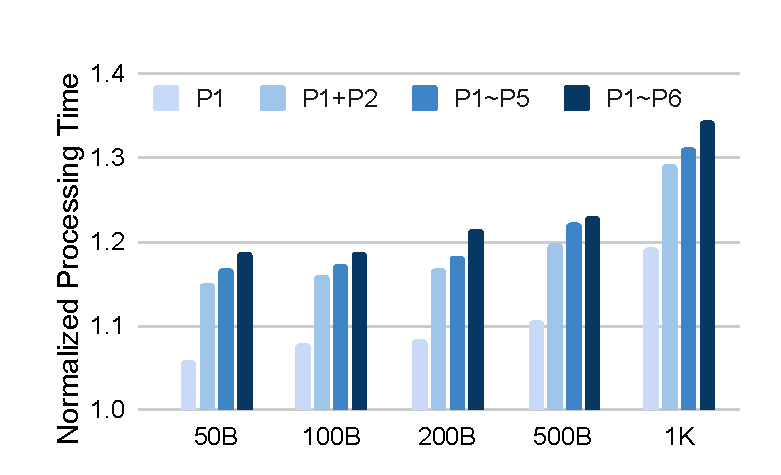
\includegraphics[scale=0.46]{figures/fg-nw-perf.pdf}
    \caption{Sequence alignment}\label{fg-nw-perf}
\end{minipage}
\begin{minipage}[t]{0.33\linewidth}
    \centering
    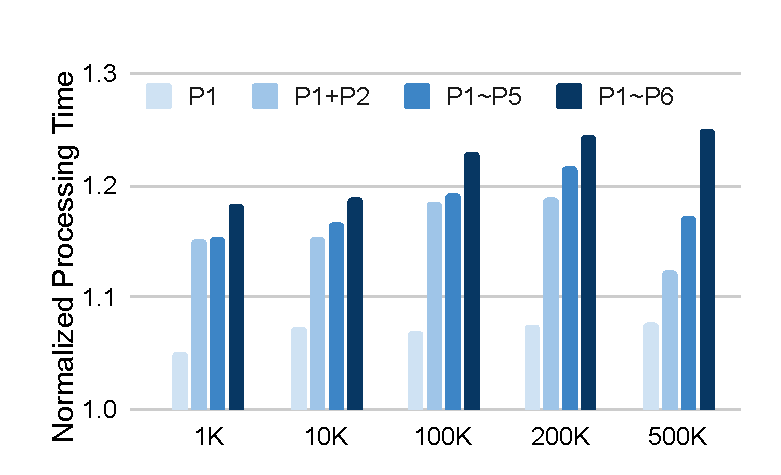
\includegraphics[scale=0.46]{figures/fg-fasta-perf.pdf}
    \caption{Sequence generation}\label{fg-fasta-perf}
\end{minipage}
\begin{minipage}[t]{0.32\linewidth}
    \centering
    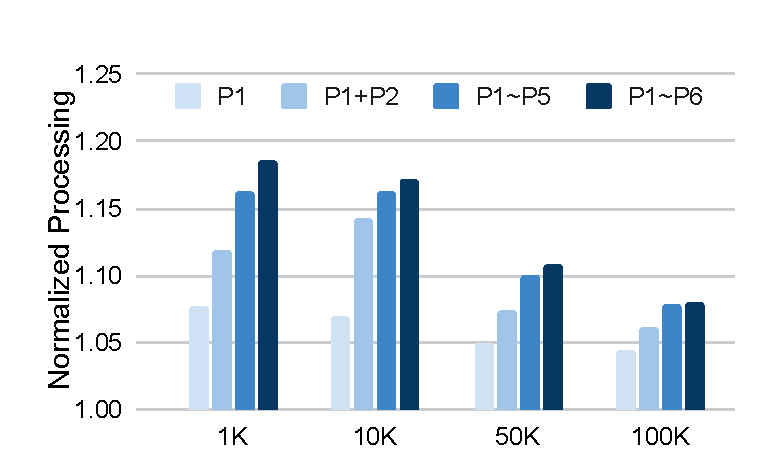
\includegraphics[scale=0.46]{figures/fg-credit-score.pdf}
    \caption{Credit scoring}\label{fg-credit-score}
\end{minipage}
\end{center}
\vspace{-12pt}
\end{figure*}
%\begin{figure}[htbp]
\centerline{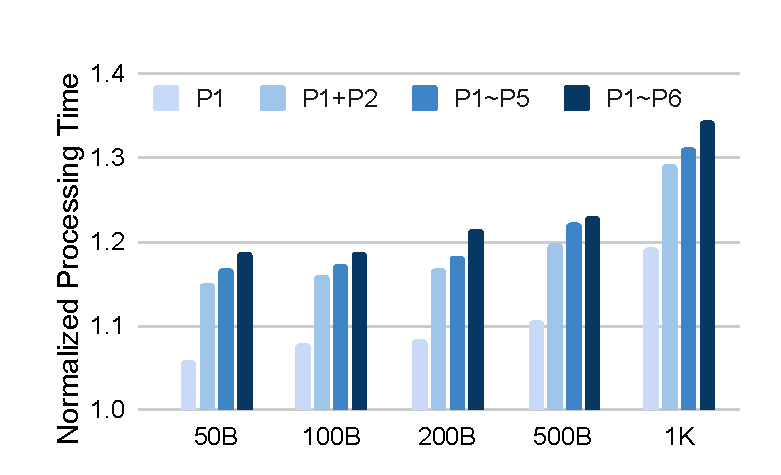
\includegraphics[scale=0.48]{figures/fg-nw-perf.pdf}}
\caption{Performance on sequence alignment}\label{fg-nw-perf}
\end{figure}
%\begin{figure}[htbp]
\centerline{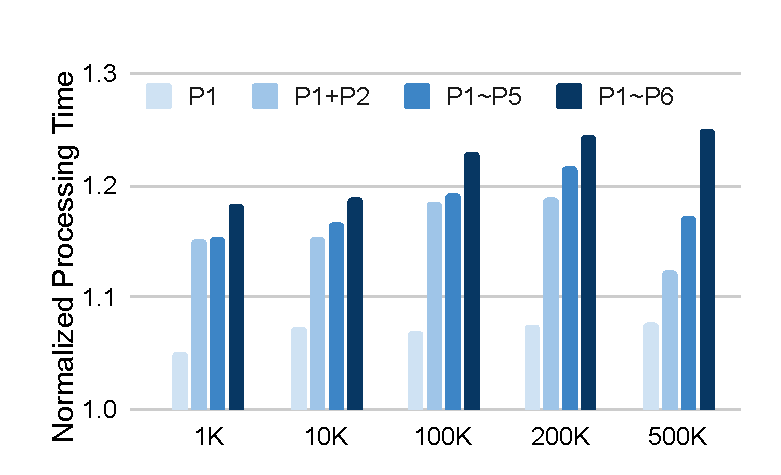
\includegraphics[scale=0.48]{figures/fg-fasta-perf.pdf}}
\caption{Performance on sequence generation}\label{fg-fasta-perf}
\end{figure}
%\begin{figure}[htbp]
\centerline{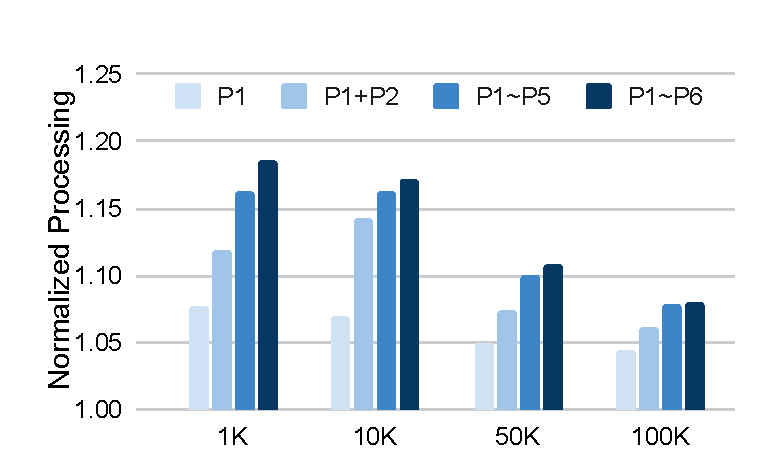
\includegraphics[scale=0.48]{figures/fg-credit-score.pdf}}
\caption{Performance on credit scoring}\label{fg-credit-score}
\end{figure}

For sequence generation, Figure~\ref{fg-fasta-perf} shows the performance when the output size (x-axis) varies from 1K to 500K nucleotides. Enforcing P1 alone results in 5.1\% and 6.9\% overheads when 1K and 100K are set as the output lengths. When the output size is 200K, our prototype yields less than 20\% overhead. Even when the side channel mitigation is applied, the overhead becomes just 25\%. With the increase of processing data size, the overhead of the system also escalates; however, the overall performance remains acceptable.
Sometimes the differences between P1+P2 and P1-P5 seem slight mainly because the instrumentations on indirect branches (P5) are few. Meanwhile, the instrumentation to enforce P1/P2 can be reused to enforce P3/P4 (via different boundaries). Thus, the performance overhead caused by P3/P4 is negligible (when P1/P2 are already enforced). 

\vspace{2pt}\noindent$\bullet$\textit{ Personal credit score analysis}. In our study, we implemented a BP neural network-based credit scoring algorithm~\cite{jensen1992using} that trains a model to calculate user's credit scores. The model was trained on 10000 records and then used to make prediction (i.e., output a confidence probability) on different test cases.
As shown in Figure~\ref{fg-credit-score}, on 1000 and 10000 records, enforcement of P1-P5 would yields around 15\% overhead. 
%Only P1+P2 takes more than 12\% herein. 
While processing more than 50000 records, the overhead of the full check does not exceed 20\%.  The overhead of P1-P6 does not exceed 10\% when processing 100K records.

\begin{figure}[htbp]
\centerline{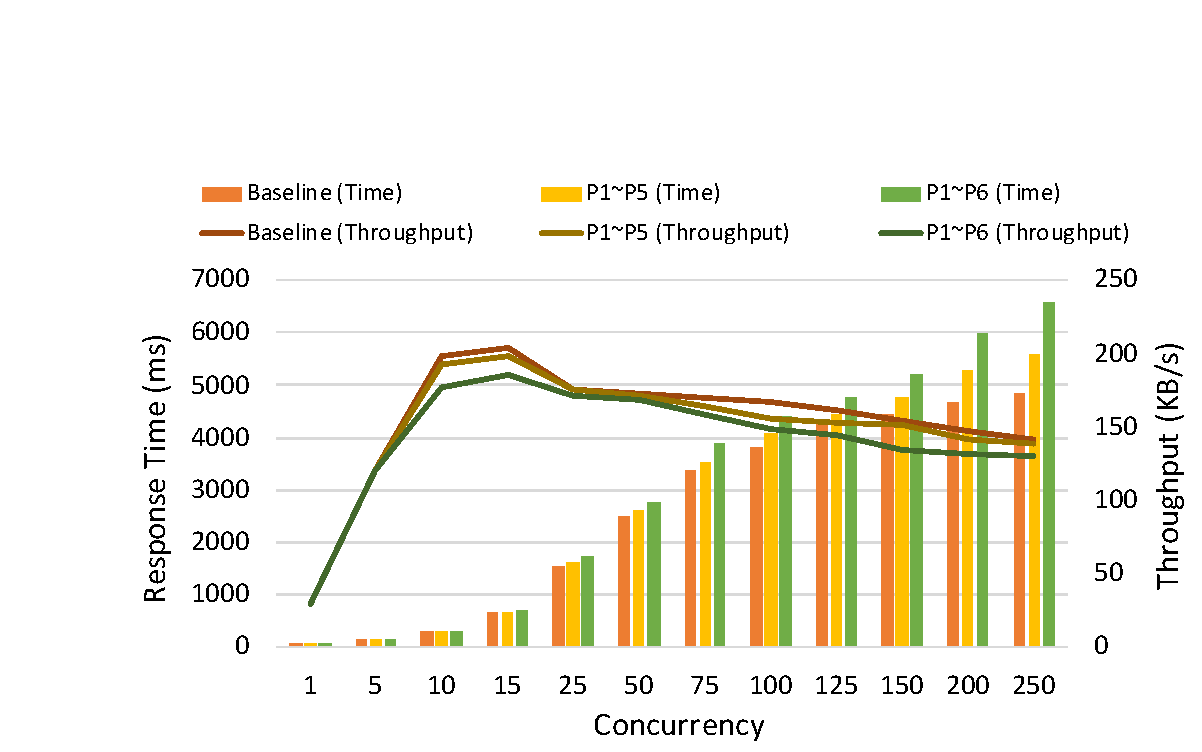
\includegraphics[scale=0.48]{figures/fg-https-server.pdf}}
\vspace{-2pt}
\caption{Performance on HTTPS server}\label{fg-https-all}
\vspace{-15pt}
\end{figure}
%\begin{figure}[htbp]
\centerline{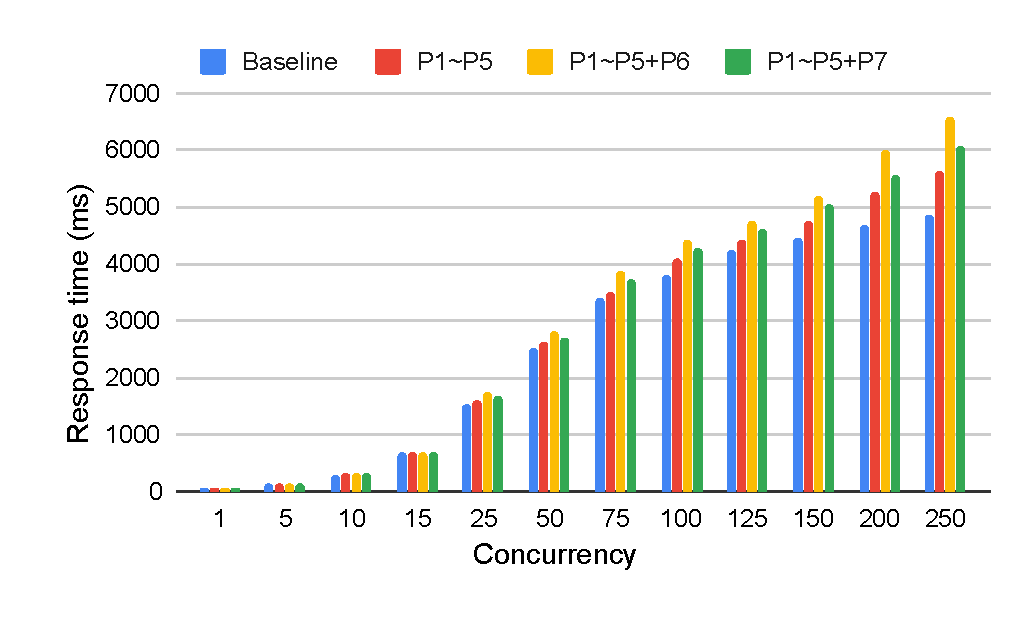
\includegraphics[scale=0.5]{figures/fg-https-rs.pdf}}
\caption{Performance on HTTPS Server (Response Time)}\label{fg-https-rs}
\end{figure}

\vspace{2pt}\noindent$\bullet$\textit{ HTTPS server}. We built an HTTPS server in enclave using the mbed TLS library~\cite{mbedtls}. The case of HTTPS server is to show that DEFLECTION is capable of handling multiple clients and it outperforms other solutions when the data size is increasing.
A client executes a stress test tool - Siege~\cite{siege} - on another host in an isolated LAN. Siege was configured to send continuous HTTPS requests (with no delay between two consecutive ones) to the web server for 10 minutes. We measured its performance in the presence of different concurrent connections to understand how our instrumented HTTPS server implementation would perform. 
%One concurrent request is deployed for measuring the response time. 

%\begin{figure}[htbp]
\centerline{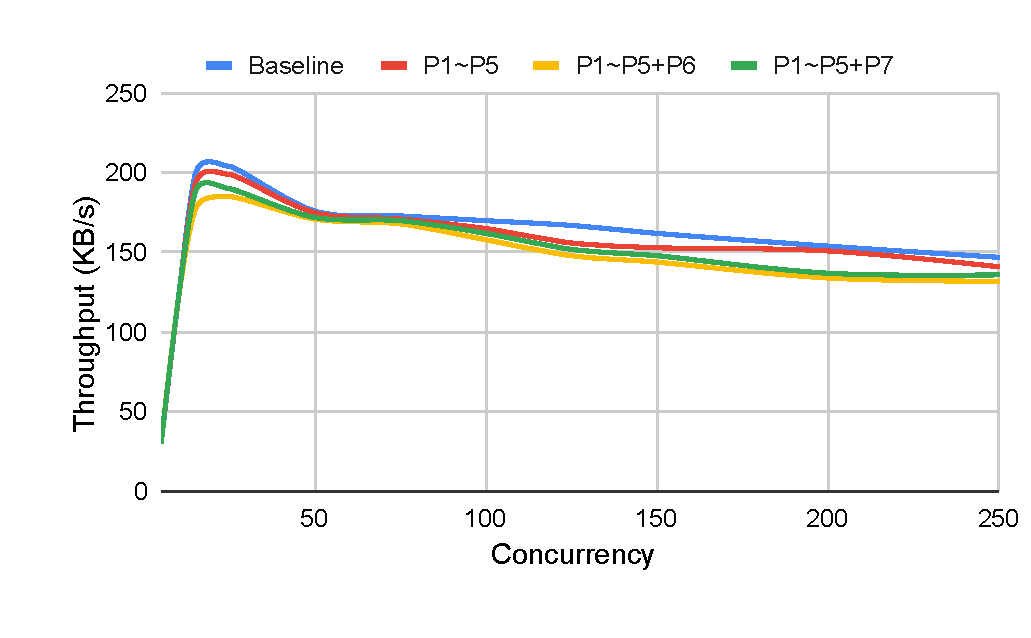
\includegraphics[scale=0.5]{figures/fg-https-tp.pdf}}
\caption{Performance on HTTPS Server (Throughput)}\label{fg-https-tp}
\end{figure}

Figure~\ref{fg-https-all} shows the response times and throughput when all policies are applied to the HTTPS server benchmark. When the concurrent connections are less than 75, the instrumented HTTPS server has similar performance of the in-enclave https server without instrumentation. When the concurrency increases to 100, the performance goes down to some extent. 
While after the concurrency increases to 150, the response time of instrumented server goes up significantly. On average, enforcing P1-P6 results in 14.1\% overhead in the response time. As for throughput, when the number of the concurrent connections is between 75 and 200, the overhead is less than 10\%. 
%the baseline always achieveshigher throughput, though just less than 10\% higher. 
These experiments on realistic workloads show that all policies, including side-channel mitigation, can be enforced at only reasonable cost. 

%proper policies on side channel mitigations can be enforced with only reasonable overhead.

\vspace{3pt}\noindent\textbf{Performance comparison on HTTPS server}.
Here we compare the performance overheads induced by existing shielding runtimes with our solution. Since Occlum has not integrated the SFI feature in its latest version~\cite{occlum} and Graphene-SGX does not support our security policies, we cannot get their performance details to compare against ours when policy-enforcing instrumentations are added. In our study, we ran an HTTPS server within those runtimes. As expected, their performance is affected by the workload, sizes of files requested from the server. As shown in Figure~\ref{fg-comparison}, unprotected Graphene-SGX has the best transfer rate with relatively small files. However, with the size growing, \textsc{Deflection} outperforms both runtimes (77\% of running the server on the native Linux), even when our approach implements security policies (P0-P5) while these runtimes do not. 


%Here we compare the performance overhead induced by existing shielding runtimes with our solution.  Since Occlum has not integrated the SFI feature in its latest version~\cite{occlum}, therefore we do not have the performance details on how it performs compared to ours when certain instrumentations were added. Compared with the HTTPS server on native Linux, shielding runtimes have performance discrepancies when requesting different sizes of files. When processing files less than 50MB, Graphene-SGX has the best transfer rate. However, it drops drastically with the file size increasing. Occlum's performance (1 thread, without SFI) also suffers from processing files whose size is larger than 70MB, while our solutions (both with and without policy enforcement) maintain a relatively high level of normalized transfer rate (greater than 77\%).


\begin{figure}[htbp]
\centerline{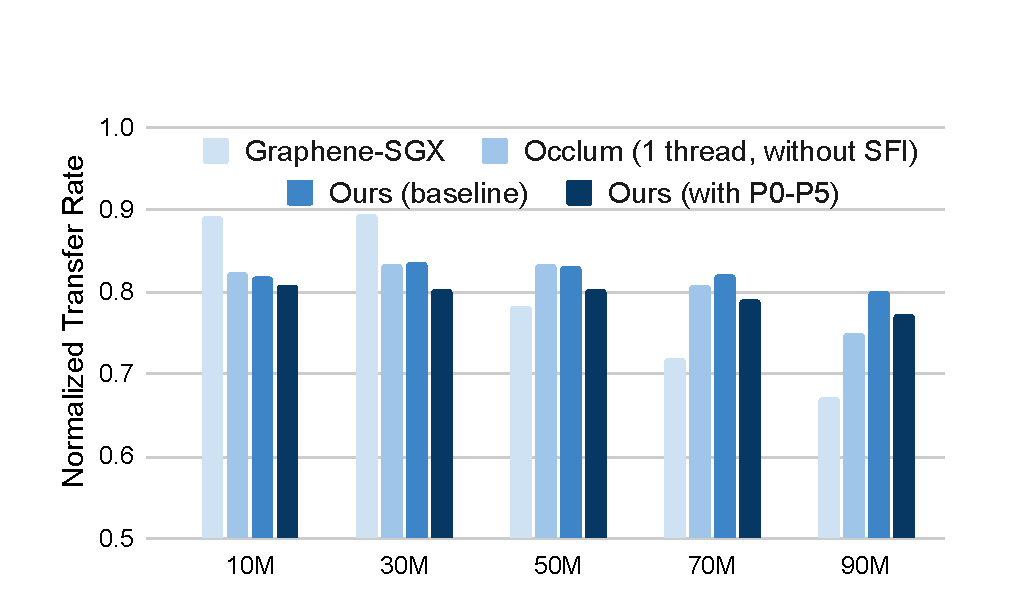
\includegraphics[scale=0.42]{figures/fg-comparison.pdf}}
\vspace{-2pt}
\caption{Performance comparison}\label{fg-comparison}
\vspace{-15pt}
\end{figure}
%\weijie{more distinguishable colors}

\ignore{
Currently, Occlum has not integrated the SFI feature in its latest version~\cite{occlum}, therefore we do not have the performance details on how it performs compared to ours when certain instrumentations were added. Compared with the HTTPS server on native Linux, Graphene-SGX, Occlum, and Ours all fluctuate between from 80\% to 90\%.
The performance of Occlum without SFI and the performance of the baseline CAT prototype (without ) are neck and neck, while Graphene-SGX has the best transfer rate since it does not provide memory access/CFI protection like ours (in Figure~\ref{fg-comparison}). Nevertheless, Graphene-SGX has to create a new enclave for each new process, which is very time consuming~\cite{shen2020occlum}.
The concurrent number ($<= 256$) has slight affect on the network throughput.
}
\section{Discussion}\label{sec-discussion}

%In previous sections we have shown that the design of CAT offers lightweight and efficient in-enclave verification of privacy policy compliance. 
%Here we discuss some extensions.

%\subsection{Preventing Side Channels}

%Side/covert channel often hides in the normal behaviors during program execution. Since the logic of service provider’s code would be very complicated, even if we could instrument all parts which needs to be protected, and guarantee the completeness of CFI policies if we do not apply side channel defenses.

%Although as described, side channel/covert channel issues are not considered in this paper, we still want to acclaim that side channel defense like CosMIX~\cite{orenbach2019cosmix} can be incorporated into our framework.
\vspace{3pt}\noindent\textbf{Supporting other side/covert channel defenses}.\label{subsec:morescenario}
The framework of our system is highly flexible, which means assembling new policies into current design can be very straightforward.
In Section~\ref{subsec-producer}, we talked about policy enforcement approaches for side channel resilience.
It demonstrated that our framework can take various side channel mitigation approaches to generate code carried with proof. Besides AEX based mitigations which we learnt from Hyperrace~\cite{chen2018racing}, others~\cite{doychev2015cacheaudit,almeida2016verifying,shih2017t,gruss2017strong,wu2018eliminating,wang2019identifying,orenbach2019cosmix} can also be transformed and incorporated into the design, \revise{specifically for mitigating cache timing, memory bus timing~\cite{liu2015can}, and other timing channels.}
\revise{ORAM~\cite{sasy2017zerotrace,ahmad2019obfuscuro} can also be integrated to \textsc{Deflection} as a policy, to relieve memory access based side- or covert- channel leakage to some extend.}
Additionally, policies such as \textit{on-demand aligning/blurring processing time} can be added for preventing processing-time based covert channels~\cite{liu2017demand}.
Even though new attacks have been kept being proposed and there is perhaps no definitive and practical
solutions to all side/covert channel attacks, we believe eventually some efforts can be integrated in our work, even using SGXv2~\cite{orenbach2020autarky}.

\ignore{
Other on-demand policies against newly-published security flaws can be appended/withdrawn to serve various goals. \textsc{Deflection} can make the quick patch possible on software level, just like the way people coping with 1-day vulnerabilities - emergency fix. 
}

%System calls may create covert channels, which also can be eliminated with more stricter policies such as fixing system call intervals.

%\weijie{Autarky: Closing controlled channels with self-paging enclaves}
%\weijie{transient execution attacks could be mitigated using other policies (e.g., inserting mfence/lfence to the service binary code)}

%\subsection{Other information leakage via deliberate interrupts issued from malicious OS}

%\vspace{3pt}\noindent\textbf{Supporting multi-user}.
%Currently we support single data owner scenarios. Of course for multi-user scenarios, we can easily add a data cleansing policy which ensures that once the task for one data owner ends, all her data will be removed from the enclave before the next owner's data is loaded, together with the content of SSA and registers, while not destroying the bootstrap enclave after use.
%Further, to fully support multi-user in-enclave services, we need to ensure each data owner's session key remains secret and to conduct remote attestation for data owners when they switch. Hardware features like Intel MPX~\cite{shen2018isolate} can be additionally applied to enforce memory permission integrity~\cite{zhao2020mptee}, as a supplementary boundary checking policy.



\vspace{3pt}\noindent\textbf{Supporting multi-threading}.
\revise{SGX supports multi-threaded execution. To concurrently service many clients, policies such as isolating each thread's private memory and setting read-only permissions on cross-thread shared memory can be enforced.}
Multi-threading could introduce serious bugs~\cite{weichbrodt2016asyncshock}. The proof enforcement of CFI may suffer from a time of check to time of use (TOCTOU) problem~\cite{xu2019confirm}.
To cope with that, we can make all CFI metadata to be kept in the register or hardware~\cite{delozier2020hurdle} instead of in memory, and guarantee that the instrumented proof could not be modified by any threads~\cite{burow2019sok}. 

%When taking multi-threading into account, the proof generation process become more complicated and cumbersome~\cite{guo2007certified}.
%\weijie{other issues}\cite{zhao2020mptee}\cite{shen2020occlum}




%\weijie{Of course, preventing memory read operations from other threads can take the multi-threading leakage once and for all. However, we do not apply this policy since it is too heavy. By enforcing enforcing policies from P1 to P5,  outside the enclave except via legitimate Ocalls.}

%Note that even we can prevent reads from other threads, that is not enough. If we don't prevent attacks mentioned in CONFirm, \weijie{multithread CFI issue}, the CFI is still broken. \weijie{enforcing P5 also cannot eliminate the threat of multi-thread CFI issue.} Therefore, we use TSX to wrap the checking code. \weijie{We need to discuss: more than 1 SSA/TLS and concurrent execution.}

%\wenhao{1. it seems that we do not need to audit memory loads, since it cannot leak; 2. , multi-thread CFI issues does not exist, as one thread cannot modify the CFI metadata? 

%\vspace{3pt}\noindent\textbf{Supporting on-demand policies}.



\section{Related Work}\label{sec-relatedwork}

\vspace{3pt}\noindent\textbf{Secure computing using SGX}.
Many existing works propose using SGX to secure cloud computing systems, e.g., VC3~\cite{schuster2015vc3}, TVM~\cite{hynes2018efficient}, by using 
sand-boxing, containers~\cite{tian2019practical}, and others~\cite{shinde2017panoply,shanker2020evaluation}. 
In-enclave JVM interpreter is also a good choice~\cite{jiang2020uranus}. These systems protect the enclave on untrusted platform, as a result, they either do not protect the code privacy or they consider a one-party scenario, i.e., the code and data needed for the computation are from the same participant. 
%In contrast, we consider 3 real world scenarios (CCaaS, CDaaS and CDCM) protecting code and data from multiple distrustful parties. 

\vspace{3pt}\noindent\textbf{Data confinement with SFI}.
Most related to our work are data confinement technologies, which confines untrusted code with confidentiality and integrity guarantees. Ryoan~\cite{hunt2018ryoan} and its follow-up work~\cite{hunt2018chiron} provide an distributed sand-box by porting NaCl to the enclave environment, confining untrusted data-processing modules to prevent leakage of the user’s input data. However the overhead of Ryoan turns out huge (e.g., 100\% on genes data) and was evaluated on an software emulator for supporting SGXv2 instructions.
XFI~\cite{erlingsson2006xfi} is the most representative unconventional PCC work based on SFI, which places a verifier at OS level, instead of a TEE. \revise{Our compiler-based generator is more efficient in providing forward-edge CFI and our runtime enforcement is simpler than inline reference monitor or dynamic binary translation used by traditional SFI}~\cite{zhou2014armlock,tan2017principles}. Occlum~\cite{shen2020occlum} is
a design of SGX-based library OS, enforcing in-enclave task isolation with \DIFaddbegin \DIFadd{an }\DIFaddend MPX-based multi-domain SFI scheme. 
Side channels pose serious threats~\cite{lee2017inferring,wang2017leaky,van2018foreshadow,chen2019sgxpectre}, while existing work assumes side channels as an orthogonal research topic~\cite{sinha2015moat,subramanyan2017formal,shen2020occlum}. 
%This leaves a challenge to integrate SGX secure computing framework with SGX side defense. 
Our framework is designed with side channels in mind and it can flexibly support integration of instrumentation based side channel defenses~\cite{shinde2016preventing,shih2017t,oleksenko2018varys,sinha2017compiler,chen2018racing}.
%As the goal of Occlum and others is not to prevent information leakage from untrusted code, none of them employs protections against side channel leakages. 
%It has a distributed verification design, the TCB introduced by the Library OS is substantial non-negligible.

\vspace{3pt}\noindent\textbf{Code privacy}.
Code secrecy is an easy to be ignored but very important issue~\cite{kuccuk2019managing}. TEEshift~\cite{lazard2018teeshift}, 
DynSGX~\cite{silva2017dynsgx} and SGXElide~\cite{bauman2018sgxelide} both make possible that developers execute their code privately in public cloud environments, enabling developers to better manage the scarce memory resources. However, they only care about the developer's privacy but ignore the confidentiality of data belonging to users. %\revise{Since the code provider will not expose any details, inferring unknown models without prior knowledge is highly impossible~\cite{tramer2016stealing}.\wenhao{do we need this sentence?}}

\vspace{3pt}\noindent\textbf{Confidentiality verification of enclave programs}.
With formal verification tools, Moat~\cite{sinha2015moat} and its follow-up works~\cite{sinha2016design} verify if an enclave program has the risk of data leakage. The major focus of them is to verify the confidentiality of an SGX application outside the enclave formally and independently. Although it is possible that the verification could be performed within a ``bootstrap enclave'', the TCB would include the IR level language (BoogiePL) interpreter~\cite{barnett2005boogie} and a theorem prover~\cite{de2008z3}. Moreover, neither of them can discharge the large overhead introduced by instruction modeling and assertion proving when large-scale real-world programs are verified.
%There are works to ~\cite{sinha2015moat,subramanyan2017formal}.

%\vspace{3pt}\noindent\textbf{Proof carrying code}.
%Our approach borrows the idea from PCC, however there are significant differences between the traditional PCC scheme and ours. Instead of using formal proof tools to generate proof annotations and verify them by a theorem prover, which cannot support large programs and has a large TCB, we let the proof generator (the customized LLVM) to provide rich control/data flow information and then check them strictly inside the enclave, which removes the compiler from the TCB and further helps saving memory consumption and performance overhead.



%Side channels have been recognized as a major threat for SGX. Attacks include cache, tlb, branch prediction, page table. Side channel defenses for SGX remains an important research problem. To the best of our knowledge, ours is the first work showing how to support verification of security policies for side channel defenses.


%The overhead for each check is far less than the solving expressions~\cite{de2008z3}, and the proof verifier does not have to traverse every execution path. XFI~\cite{erlingsson2006xfi} is the most representative unconventional PCC work, which places a verifier at OS level for minimizing the TCB. 
%However, it's problematic that XFI only protects forward edge control-flow integrity. 
%However, if we apply XFI to verify an SGX program but build a verifier as a kernel module inside the OS, it makes the scheme meaningless since the OS is also not trustworthy. 
%Another similar work to reduce the TCB greatly is the Flicker~\cite{mccune2008flicker}, which is a TPM-based solution to execute security-sensitive code in isolation from an OS.
%Unlike traditional methods including a VCGen into its trusted part~\cite{necula1997proof}, in our design, we let the proof generator (the customized LLVM) to provide rich control/data flow information and then check them strictly inside the enclave, which removes the compiler from the TCB and further helps saving memory consumption and performance overhead.


%while its confinement overhead is sometimes high (100\% on Genes data) and the checkpoint restore overhead is significant (55\% on Genes data) with SGXv2 instruction emulation. 



\ignore{
Many existing works have proposed approaches to perform privacy-preserving computation tasks or constitute a computing environment. There are quite some solutions using cryptography, e.g., fully homomorphic encryption (FHE)~\cite{gentry2009fully} that allows a computing task to be executed directly on encrypted data
%, and secure multi-party computation~\cite{jha2008towards} that enable different parties to jointly perform a computing task without disclosing their individual inputs to the others. 
However, these techniques often could not scale to meet the requirements for running complicated tasks.

A more scalable alternative solution is TEE, especially Intel SGX, which can run as fast as CPU allows except some small overheads introduced by encryption, decryption, and authentication~\cite{gueron2016memory}, and therefore can potentially achieve a performance that comes close to native execution (within one order of magnitude slowdown~\cite{tramer2018slalom}). 
Researchers proposed VC3, the first system that allows users to run distributed MapReduce computations in the cloud while keeping their code and data always encrypted~\cite{schuster2015vc3}. From then on, there are works to verify if a program has the risk of data leakage~\cite{sinha2015moat,subramanyan2017formal}.
TVM is also a Privacy-preserving Machine Learning framework that can be used on SGX\cite{hynes2018efficient}. But in threat models of theirs, the remote user owns both data and code, which means the code may not be attestable for confidentiality.
%\weijie{To the best of our knowledge, CAT seems not the first approach that can protect both code and data privacy, while keeping the enclave is attestable. The first one should be the VC3~\cite{schuster2015vc3}, but VC3 only can protect map-reduce like services. In VC3, both E- and the user's data are always kept encrypted.}
Ryoan~\cite{hunt2018ryoan} and its follow-up work~\cite{hesamifard2018privacy} provide an SFI-based distributed sandbox, confining untrusted data-processing modules to prevent leakage of the user’s input data, while its confinement overhead is sometimes high (100\% on Genes data) and the checkpoint restore overhead is significant (55\% on Genes data) with SGXv2 instruction emulation. 
MPTEE~\cite{zhao2020mptee} also introduces a loader and a trampoline table to ensure the dynamic changing of page privileges. And it applies some boundary check mechanisms like Intel MPX~\cite{shen2018isolate} to enforce memory permission integrity. Similar work such as Occlum~\cite{shen2020occlum} can also guarantee a secure and efficient multitasking environment.
%Moreover, those approaches do not take side channel leakage into consideration, which would be a threat to confidentiality partially.
%Researchers use SGX and other hardware features (Intel MPX) to build a multi-domain software fault isolation (SFI) scheme\cite{shen2018isolate}, which can isolate data and code domains.

However, if we only depend on SGX's built-in integrity protection mechanism - the RA protocol - the in-enclave code would be still unreliable and there is no privacy since the code must be public for attestation.
%\weijie{talk about the code privacy}
Code secrecy is is an easy to be ignored but very important issue~\cite{mazmudar2019mitigator,kuccuk2019managing}.
DynSGX~\cite{silva2017dynsgx} and SGXElide~\cite{bauman2018sgxelide} both make possible that developers execute their code privately in public cloud environments, enabling developers to better manage the scarce memory resources. However, they only care about the developer's privacy but ignore the confidentiality of data belonging to remote users. 


%Many works have pursued to reducing the system TCB. Glamdring~\cite{lind2017glamdring} can automatically partition the application into untrusted and trusted parts for SGX, reducing the TCB. But still, it does not care about the Intellectual Property of the developer's code.

%\weijie{the following work also do not consider the code privacy}

Although we learn from the principle of PCC to implement our scheme, there are some significant differences between the traditional PCC scheme and ours. Traditional PCC usually uses the theory of formal proof to abstract a model, generate proof annotations and verify them by a theorem prover. Such formal verification still has two limitations: the degree of automation (complex implementation) and the degree of availability (inadequate expressiveness)~\cite{d2008survey}. Instead, our scheme does not use the formal method but leverages the control/data flow analysis. The overhead for each check is far less than the solving expressions~\cite{de2008z3}, and the proof verifier does not have to traverse every execution path. XFI~\cite{erlingsson2006xfi} is the most representative unconventional PCC work, which places a verifier at OS level for minimizing the TCB. 
%However, it's problematic that XFI only protects forward edge control-flow integrity. 
However, if we apply XFI to verify an SGX program but build a verifier as a kernel module inside the OS, it makes the scheme meaningless since the OS is also not trustworthy. 
Another similar work to reduce the TCB greatly is the Flicker~\cite{mccune2008flicker}, which is a TPM-based solution to execute security-sensitive code in isolation from an OS.
Unlike traditional methods including a VCGen into its trusted part~\cite{necula1997proof}, in our design, we let the proof generator (the customized LLVM) to provide rich control/data flow information and then check them strictly inside the enclave, which removes the compiler from the TCB and further helps saving memory consumption and performance overhead.

}
\section{Conclusion}\label{sec-conclusion}

In this paper we proposed \textsc{Deflection}, which allows the user to verify the code provided by untrusted parties without undermining their privacy and integrity. Meanwhile, we instantiated the design of a code generator and a code consumer (the bootstrap enclave) - a lightweight PCC-type framework.
\DIFdelbegin \DIFdel{Due to the differences between normal binary and SGX binary, we retrofit the framework to be fitted into SGX. In return, we reduce the framework's TCB as small as possible.
}\DIFdelend %DIF >  Due to the differences between normal binary and SGX binary, we retrofit the framework to be fitted into SGX. In return, we reduce the framework's TCB as small as possible.
%by moving the compiler out of the trusted part.
Our work does not use formal certificate to validate the loaded private binary, but leverage data/control flow analysis to fulfill the goal of verifying if a binary has such data leakage, allowing our solution to scale to real-world software. 
%Moreover, our method provides a new paradigm for PCC to use a TEE (other than the OS) as an execution environment, which provides more powerful protection. 


%A coarse grained CFI is enforced to prevent a strong attacker from bypassing the runtime checks we instrumented in the loaded binary.  The verifier we built is self-protection and is hard to be circumvented.
%Our CFI scheme can guarantee all indirect branches the target binary and the SGX’s SDK are legal.  

%In this way, we can ensure that the trust chain is sound and complete.

%In future, we plan to extend the framework to support other policies.
%using typed assembly language~\cite{morrisett1999system}

%\revise{Our design does have a few limitations, however.}

\section*{Acknowledgment}

%\normalem

% \clearpage
% commenting all appendices for now

\bibliographystyle{./bibliography/IEEEtran}
%\bibliographystyle{plain}
\bibliography{./bibliography/IEEEabrv,./bibliography/ref}

%\clearpage
%\appendix

%for ACM format
%\section*{Appendix}

%\weijie{illustrate the alternative side/covert channel mitigation policy}

\subsection{Instrumentation Details}\label{appendix-instrumentation}

Here we illustrate other instrumentation modules in our code generator.

\vspace{3pt}\noindent\textbf{RSP modification instrumentation}. Since RSP spilling would cause illegal implicit memory writing, RSP modification instructions should also be checked. This module first locates all RSP modification instructions in the program and then instruments assembly code after them to check whether the RSP values are out of bounds. Just like store instruction instrumentation, the upper and lower boundaries of RSP are specified by the loader and written into the assembly instructions by the rewriter, while the compiler only fills them with speical immediates (0x5ffffffffffff and 0x6ffffffffffff).

When the instrumentation finds that the stack pointer is modified to an illegal address, it will cause the program to exit. Fig.~\ref{fg-rsp} shows eight instructions be inserted after the \texttt{ANDQ} instruction, which is tend to reserve new stack spaces (minus 16 from the value in RSP register). We leave the enforcement of implicit modification of the stack pointer using \texttt{PUSH} and \texttt{POP} by adding guard pages (a page with no permission granted) to the dynamic loader.

\begin{figure}[hbp]
\begin{center}
\begin{minipage}{0.4\textwidth}
\begin{lstlisting}[basicstyle=\scriptsize,numbers=left]
andq    $-16, %rsp
pushq   %rax
movabsq $0x5FFFFFFFFFFFFFFF, %rax   ;set bounds
cmpq    %rax, %rsp
ja      exit_label
movabsq $0x6FFFFFFFFFFFFFFF, %rax   ;set bounds
cmpq    %rax, %rsp
jb      exit_label
popq    %rax
\end{lstlisting}
\end{minipage}
\end{center}
\caption{RSP Modifying Instrumentation}\label{fg-rsp}
\end{figure}

\vspace{3pt}\noindent\textbf{Indirect branch instrumentation}. For checking indirect branches, we first extract all legal target names at assembly level, and output them to a list. 
%The start address of this list in enclave memory is rewritten to certain values by the Imm rewriter when used. 
After that, we insert a inspection function calling in front of every indirect branch instruction (in Fig.~\ref{fg-indirect}), to achieve forward-edge CFI check at runtime. 
Specifically, the inspection function \verb|CFICheck| is written and included in the target binary, to search if the indirect branch is on that list, therefore ensuring they conform to the program control flow. 
%Consequently as shown in Fig.~\ref{fg-indirect}, calling these functions in assembly will achieve legality checks on the program at runtime.

\begin{figure}[hbp]
\begin{center}
\begin{minipage}{0.3\textwidth}
\begin{lstlisting}[basicstyle=\scriptsize,numbers=left]
movq	%reg, %rdi
callq	CFICheck
\end{lstlisting}
\small{Instrumentations before callq \*\%reg}
\end{minipage}
\begin{minipage}{0.3\textwidth}
\begin{lstlisting}[basicstyle=\scriptsize,numbers=left]
movq	(%reg), %rdi
callq	CFICheck
\end{lstlisting}
\small{Instrumentations before callq \*(\%reg)}
\end{minipage}
\end{center}
\caption{Indirect Call Instrumentation}\label{fg-indirect}
\end{figure}

\vspace{3pt}\noindent\textbf{Shadow stack}. For function returns, the code generator instruments instructions to support a shadow call stack, which is a fully precise mechanism for protecting backwards edges~\cite{burow2019sok}. The shadow stack’s base address is specified by the loader, and will be rewritten by the Imm rewriter (to replace the imm filled in by the compiler in advance).

As shown in Fig.~\ref{fg-shadowstack}, at every function entry, we insert instructions (before the function stack alignment) that will modify the shadow stack top pointer and push the function's return address into the shadow stack. Similar to instrumentation at the function entry, instructions inserted before the function returns  modify the stack pointer and pop the return address. Comparing the saved return address with the real return address, \texttt{RET} can be checked at runtime.

\begin{figure}[hbp]

\begin{center}
    
\begin{minipage}{0.3\textwidth}
\begin{center}
\begin{lstlisting}[basicstyle=\scriptsize,numbers=left]
movabsq	$0x2FFFFFFFFFFF, %r11
addq	$8, (%r11)
movq	(%r11), %r10
addq	%r10, %r11
movq	(%rsp), %r10
movq	%r10, (%r11)
pushq	%rbp
movq	%rsp, %rbp
\end{lstlisting}
\small{Instrumentation before stack alignment}
\end{center}
\end{minipage}

\hfill

\begin{minipage}{0.3\textwidth}
\begin{center}
\begin{lstlisting}[basicstyle=\scriptsize,numbers=left]
movabsq	$0x2FFFFFFFFFFF, %r11
movq	(%r11), %r10
addq	%r11, %r10
subq	$8, (%r11)
movq	(%r10), %r11
cmpq	%r11, (%rsp)
jne	exit_label
\end{lstlisting}
\small{Instrumentation before function return}
\end{center}
\end{minipage}

\hfill

\begin{minipage}{0.3\textwidth}
\begin{center}
\begin{lstlisting}[basicstyle=\scriptsize,numbers=left]
exit_label:
    movl    $0xFFFFFFFF, %edi
    callq   exit
\end{lstlisting}
\small{Instrumentation for exit label}
\end{center}
\end{minipage}

\caption{Structured Guard Formats of Shadow Stack}\label{fg-shadowstack}

\end{center}
\end{figure}

\vspace{3pt}\noindent\textbf{SSA monitoring instrumentation}. 
As demonstrated in previous works~\cite{gruss2017strong,chen2018racing}, AEX can be detected by monitoring the SSA. Therefor, to enforce P6, we instrument every basic block to set a marker in the SSA and monitor whether the marker is overwritten by AEX within the basic block. The execution is terminated once the number of AEXes within the basic block exceeds a preset threshold. 

A function is also implemented to get the interrupt context information in the bootstrap enclave's SSA area. At the beginning of each basic block, we call this function through instrumentation to check whether there are too many interruptions during execution. When a basic block is too large, this function will also be called in the middle of basic block every k ($k=20$) instructions. We count the number of interrupts/AEXs that occurred from the last check to the current check. When 22 or more are triggered, the target program aborts.

\vspace{3pt}\noindent\textbf{Alternative instrumentation}. 
To mitigate AEX based side-channel risks, CAT-SGX provides an alternative enforcement mechanism, through TSX, which can be chosen when compiling the target program. This approach is based upon T-SGX~\cite{shih2017t}, putting transaction memory protection on each basic block and running a fallback function to keep track of the number of interrupts observed. Just like T-SGX, when more than 10 consecutive AEXes happen, the computation aborts, due to the concern of an ongoing side-channel attack.  The protection is instrumented by the generator and its presence is verified by the code consumer in the enclave. 

We have implemented a function, in which \texttt{XBEGIN} and \texttt{XEND} is called and fallback is specified, which can be inserted into the target binary. Around each branch, every \texttt{CALL}/\texttt{RET} instruction, and at the begin/end of each basic block, we call this function so that the program leaves the last transaction and enters a new transaction when a possible control flow branch occurs and completes. Some code snippets are shown in Figure~\ref{fg-tsgx}. 

%About wrapper function
To deal with the compatibility problems caused by calling functions that has no need to be checked (e.g., the system calls via OCall stubs), we implemented another non-TSX wrapper for external functions.
Particularly, our LLVM pass will generate an alternative function \verb|wrapper_foo| to replace original function \verb|foo|, to avoid the TSX instrumentation.
%wrapper function is not the tsx wrapper

\begin{figure}
\begin{center}
% \begin{minipage}{0.3\textwidth}
% \begin{lstlisting}[basicstyle=\scriptsize,numbers=left, numberstyle=\scriptsize,,keywordstyle=\color{blue!70},commentstyle=\color{red!50!green!50!blue!50}, rulesepcolor=\color{red!20!green!20!blue!20}]
% xend
% movq	%r15, %rax
% \end{lstlisting}
% \end{minipage}

% \footnotesize{Instrumentation at the beginning of each branch instruction}

% \begin{minipage}{0.3\textwidth}
% \begin{lstlisting}[basicstyle=\scriptsize,numbers=left, numberstyle=\scriptsize,,keywordstyle=\color{blue!70},commentstyle=\color{red!50!green!50!blue!50}, rulesepcolor=\color{red!20!green!20!blue!20}]
% movq	%rax, %r15
% call    transactionBegin
% \end{lstlisting}
% \end{minipage}

% \footnotesize{Instrumentation before function return}

\begin{minipage}{0.3\textwidth}
\begin{lstlisting}[basicstyle=\scriptsize,numbers=left]
movq	%rax, %r15
lahf
movq	%rax, %r14
callq	transactionEndBegin
movq	%r14, %rax
sahf
movq	%r15, %rax
\end{lstlisting}
\end{minipage}

\end{center}
\caption{TSX instrumentation}\label{fg-tsgx}
\end{figure}

\subsection{Preparing Target Binary}\label{appendix-preparing}

\vspace{3pt}\noindent\textbf{Libc}. To manage interactions with the untrusted operating system, we make some Ocall stubs for system calls. 
Related works~\cite{shinde2017panoply,tsai2017graphene,priebe2019sgx,shinde2020besfs} provide various great Ocall interfaces. But some of them still require additional interface sanitizations.
We use parts of musl libc~\cite{musllibc} for completing the code loading support (Section~\ref{subsec:code-loading-support}).
%- since we cannot use SGX SDK's Libc, we make the applications calling Musl-Libc and let Musl to call the customized 36 Ocall stubs. 
Undoubtedly, the musl libc should be instrumented as well. Then, it can be linked against other necessary libraries statically, e.g., mbedTLS for buiding an HTTPS server.

\vspace{3pt}\noindent\textbf{Stack and heap}. We also reserved customized stack and heap space for the target program execution. During the above-mentioned loading phase, the CAT-SGX system initializes a 4 MB (by default) memory space for the stack, and links against a customized and instrumented \verb|malloc| function for later heap usage. In current version of our prototype, the memory ranges of the additional stack and the heap provided for the target program are fixed, for efficient boundary checking.

\vspace{3pt}\noindent\textbf{Other necessary functions}. The instrumented proof includes not only the assembly instructions. Some necessary functions and objects also should be compiled and linked.
Since we need an algorithm to check if the address of an indirect branch target is on the legal entry label list (for P5 enforcement), a binary search function \verb|CFICheck| is inserted into the target program.
Similarly, as we need a function to enforce P6, necessary functions need to be called for SSA monitoring frequently. 
Those objects would also be disassembled and checked during the stage of proof verification, to ensure that these can not be compromised when they are called.
%, and the variables in them will not be tampered with.
%\weijie{CFICheck.o for forward-edge CFI; TransactionBegin.o and telib\_t.o for side channel resilience}

%As we retrofit the T-SGX and Hyperrace, two necessary functions (one for executing the \texttt{XBEGIN} instruction and the other for calling an SSA modification check) need to be called frequently. Therefore, objects used in side channel defenses like \verb|telib_t.o| (for SSA monitoring) that consist of those two functions respectively are linked and work with the whole instrumentations. Those objects would also be disassembled and checked during the stage of proof verification. We can ensure that these are also safe when they are called, and the variables in them will not be tampered with.
%% \onecolumn
\section*{Reviews and Summary of Revision}

\noindent Following are the reviews we received from our latest submission to IEEE S\&P 2020, and our summary of changes following the reviews.

\section{Summary of revision}
Following the reviews from IEEE S\&P 2020, we have made the following major improvements to this paper.


\vspace{3pt}\noindent\textbf{Better highlighted the novelty}.
We elaborated the strengths of our work (Section~\ref{sec-introduction}) and compared them with the most related works (Section~\ref{sec-relatedwork}). To the best of our knowledge, we are the first one proposing the CAT model and trying to address the confidential attestation dilemma (that the service code provider is reluctant to expose the implementation details of its services for public attestation) with the unbalanced proof carrying code framework. Barely related work takes into account the privacy issues of both code providers and data owners. Works such as Ekiden~\cite{cheng2018ekiden} provide a computing environment for running a smart contract on sensitive data privately. However, they only care about the confidentiality of the input data and the contract state, but don't need to cope with the secrecy of contract(program) because of its transparency. Thus, the CAT model solves a disparate problem in a totally different scenario.

Fortunately, the confidential attestation challenge can be addressed perfectly using Proof Carrying Code (PCC) framework.
According to the XFI~\cite{erlingsson2006xfi}, a brilliant work co-authored by the designer -  George C. Necula, XFI modules can be seen as an example of proof-carrying code, even though they do not include logical proofs. Similar as XFI, our work uses static analysis with inline software guards that perform checks at runtime, which could be regarded as an example of PCC that trusts only the verifier, not the means of proof generation.

Sand-boxing is a suitable technique to perform privacy-preserving computations. Related works like Ryoan~\cite{hunt2018ryoan} leverage Google NaCl to build its prototype, whose core library is about 19 MB including several LLVM components. Instead, our implementation is more lightweight, adding about 2MB of binary code to the TCB.

On the other side, our approach is more practical compared with formal methods, e.g., a type-safe language. A type-safe language compiler/interpreter along cannot finish the verification of properties such as confidentiality.  A verification condition generator (VCGen) and a proof solver should work together with the compiler/interpreter, which introduce huge TCB and computation overhead.
In our design, we let the proof generator (the customized LLVM) to provide rich control/data flow information and then check them strictly inside the enclave, which removes the compiler from the TCB and further helps saving memory consumption and performance overhead. And we fully considered the characteristics of policy-compliant computations before proposing our design. Real-world applications often contain hundreds of lines of code, and thousands of instructions. Comparing to formal verification, generating security annotations is significantly less weighted, allowing our solution to scale to real world software of such amount of code.


\vspace{3pt}\noindent\textbf{Added more policies}. We extended the number of policies that we need to enforce from 5 to 7, to fully protect the privacy of user data. These policies include data leak control, control-transfer management, self-modifying code block, and side/covert channel mitigation. We used the implemented prototype to demonstrate how policies can be enforced (using an unbalanced design of assembly level instrumentations on the code provider side with a lightweight verification on the code consumer side). 

Those additional policies including input/output constraint (P0) and side/covert channel mitigation (P6) are described (Section~\ref{subsec-policies}), which are designed to limit the amount of information an attacker can get. Specifically, attackers can not access the plaintext of input/output message directly via enforcing P0. We made OCall stubs for calling system calls. Restrictions on the length of OCall stubs can handle the issue of the Intel SGX SDK's Null-terminated string.
Enforcing P6 could protect the data owner from page fault-based controlled channel attacks and most L1/L2 cache-based side channel attacks. 
Meanwhile, Data Execution Prevention (DEP) can not be skipped since the loaded binary will be allocated on enclave's heap memory, leading to a W+X problem. The goal of enforcing DEP (P4) was elaborated in Section~\ref{subsec-policies}. This will not be a problem in SGXv2 since dynamic memory management of EPC is introduced in the new version of SGX hardware, which can protect dynamic loaded pages with permission changing and verifying instructions such as \texttt{EAUG/EMODPE/EACCEPT}.


\vspace{3pt}\noindent\textbf{Enriched implementation details}.
We added details on how the proof is generated and how the whole system works (Section~\ref{sec-implementation} and Appendix~\ref{appendix-instrumentation}). Specifically, we illustrate how to use CAT to implement information release prevention policies and common SGX side/covert channel alleviation policies. 

We built an assembly-level PCC framework from scratch. The instrumentation module for enforcing P1 and also be used in enforcing DEP, aka. P4, with few modification.
We showed that the code generator consists of portable components, which introduces a great flexibility for supporting replaceable policies. Wider policies can be integrated via implementing other LLVM passes.

Exquisite implementation was applied in building one bootstrap enclave as well (Section~\ref{subsec:bootstrap-impl}). We illustrated how the loader and the verifier can be integrated seamlessly (Section~\ref{subsec-loading}). The binary parsing module in the loader (in Figure~\ref{fg-workflow}) is  not only designed for assisting to get offsets for relocation, but also can give the program entry for later disassembling. Moreover, legal indirect branch labels need to be translated by the binary parser. The loader and the verifier formed a whole and work in harmony.

Our implementation did not use two enclave for separating the verification stage and the code loading and execution stage. The only advantage of using two enclaves is that there will be no W+X issue during the target binary loading, which actually can be dealt with the software DEP. Meanwhile, using two enclave may induce more communication overhead. The attestation protocol should be re-designed, while introduces larger TCB and more overhead since more parties are involved.
%More importantly, if we consider it more carefully, it still needs a binary rewriter within the one bootstrap enclave. 

We believe both designs are reasonable. However, at this time, we may stick to the original ``one-enclave'' design for the following reasons. Firstly, memory store operation instrumentation can be easily extended to support W+X. Secondly, within the one-enclave design, the code of resolving symbols (during loading) can be easily reused by the rewritter and the verifier which reduces the memory consumption of limited enclave memory. 
%One-enclave design is more compact and cute, which leads a smaller TCB.


\vspace{3pt}\noindent\textbf{Thoroughly evaluated the CAT system}.
We built more benchmarks (including micro-benchmarks and real-world applications) and tested them with the prototype we implemented (Section~\ref{subsec-experiments}). Performance analysis was given, showing the difference under multiple granularities of protections (P1, P1+P2, P1\textasciitilde P5, and P1\textasciitilde P6). Security suggestions on which policies should be incorporated can be made according to their performance and what security properties they can bring in at different scenarios.

In addition, the TCB of our CAT system was evaluated. Policies had been analyzed for soundness and completeness as well (Section~\ref{subsec-securityanalysis}). 
The goal of enforcing policies on memory write operations is to build an information confinement, and a CFI policy can gruarantee the check on other policies cannot be circumvented.


\vspace{3pt}\noindent\textbf{Better summarized the lessons learnt}.
We have to acknowledge that our current CAT-SGX system has limitations and we discussed them in Section~\ref{sec-discussion}. We summarized those limitations as follows.

Side channels have been recognized as a major threat for SGX. Attacks include cache, TLB, branch prediction, page table, etc. Side channel defenses for SGX remains an important research problem. 
%To the best of our knowledge, ours is the first work showing how to support side channel defenses verification by flexible security policy enforcement.
With the help of SSA monitoring to detect and prevent AEX-based channels, our work can limit the data leakage via most interrupt-based covert channels. Further, covert channel based on parameters of system calls can be eliminated by enforcing P0 - a strong constraint on input/output messages that only allows certain syscalls (\texttt{send/recv}). System functions like setjmp/longjmp are disallowed in our system since they can break
call-return semantics.
System call interval can not be a covert channel in CDaaS cases since we only process input/output once during the in-enclave service. Individual request can only leak few bits. However, it can be a threat in CCaaS scenarios such as web-server as a service. Attackers can deliberately construct requests which would cost different processing time, and transfer some secrets via the processing time difference. Overall, we have to admit that our work cannot take over all kinds side/covert channels, policies to defend against them (e.g., fixed processing time) can be added into our framework though.

Multi-threading/Multi-user is not supported currently, but can be accomplished with certain extensions. We elaborated how our work can be extended towards solving those issues in Section~\ref{sec-discussion}. Supporting the single-thread multi-user scenario could be very easy by adding a data cleansing policy as well as a session key management for multiple users. Unfortunately, supporting a multi-thread scenario would take much more effort. 
Recent works have been proposed on this hot topic. Occlum~\cite{shen2020occlum} and MPTEE~\cite{zhao2020mptee} both leverage Intel MPX~\cite{shen2018isolate} to isolate the address space between multiple threads for multitasking efficiently. Although, incluing LibOS into the TCB may not be accepted, we can learn from them and  memory read auditing policies for reserved regions for different threads. Specifically, the code provider can divide the `.data' section of the target program into memory spaces for $N$ threads.
Then on the bootstrap enclave side, the loader should keep the upper/lower bounds when performing thread switch, and the verifier can enforce the memory accessing policies for all $N$ threads.


%%%%%%%%%%%%%%%%%%%%%%%%%%%%%%%%%%%%%%%%%%%%%%%%%%%%%
%reviews

\section{Reviews}

\begin{markdown}
## Review A
=================================================


### Brief Paper Summary  

The paper proposes CAT, an approach for ensuring to a user that code meets privacy requirements without the user observing the code.  CAT relies on a combination of compiler modification to generate code that meets the privacy requirements and an SGX enclave that loads and execute the code only after verifying it meets the requirements.

### Strengths

Ensuring data privacy is important.

### Weaknesses

There is a huge gap between what the paper promises and what it delivers
Considering what is being delivered, it's not clear what the novelty is.

### Detailed Comments for Authors

Thank you for submitting your work to IEEE SP.  While I appreciate the amount of work that went into CAT, I am afraid that I cannot recommend that the work be accepted.

The paper starts with a promise of a framework that can validate the compliance of code with privacy policies. However, it only investigates a single privacy policy. There is absolutely no discussion of how the research can be extended to other privacy policies, and such extensions do not seem trivial.

The privacy policy the paper claims to enforce is to ensure that data is not leaked from the enclave.  The paper reduces this policy to five requirements (P1-P5, Page 6).  While I agree that all requirements are necessary for enforcing the policy, I am not convinced that they are sufficient.  In particular, I do not see that these requirements are sufficient to prevent data from one query leaking into another.  In the case of a service provider that provides a service to multiple clients, this would allow leaking information between clients.  Another potential information leak is via system calls or their arguments - the paper indicates that system calls are supported but does not explain how their arguments are validated.

When reducing the problem to only maintaining the five requirements, it is not clear what the advantage of the suggested approach over using type-safe languages or mechanisms such as suggested for Google Chrome Native Clients (Yee et al. IEEE SP 2009).

Side channel attacks are considered out-of-scope for the paper. However, given the vulnerability of SGX to such attacks, and the attempt to protect from malicious code, ignoring these seem to render CAT completely useless for protecting privacy.

There is absolutely no discussion of the limitations of the approach. Can the verified code communicate with the service provider? Can it use longjmp? Is multithreading supported? etc.

Overall, I think that the idea is promising, but the gap between the promise and the current implementation is too wide.  I suggest that the authors work on reducing the gap e.g. by showing how the approach could apply for a wider range of security/privacy policies.



## Review B
=================================================



### Brief Paper Summary

This paper proposes to solve a problem with remote attestation as used in SGX. One party provides code and another provides data; neither wants to provide their part in the clear; but the party providing data needs to be sure that their data's privacy is assured.  They propose to do this with a loader enclave that checks and runs proof-carrying code (PCC) guaranteed to comply with the privacy policy.

### Strengths

The system is relatively simple.

### Weaknesses

The simplicity of this system comes from its lack of expressiveness, and fixed not-very-useful security policy.

The lack of covert channel protection is very problematic.  There's not much point in blocking the front door if the back door is wide open.  While unintentional side channels can be tricky to exploit, covert channels are really easy.

The only supported policy is that no data is written outside the enclave.  It is not clear how the loader will determine whether the results of the computation comply with any kind of privacy policy, which is implied in some of the suggested use cases.  In fact, the paper doesn't discuss how output is to be produced at all, though I assume that the loader would have a trusted output routine of some kind.

The paper is riddled with typos.

This isn't proof-carrying code.  It's instrumented code.

I'm not clear why this would be better in practice than a LISP interpreter with some security/privacy policy annotations.  If you must run binary code, why must the loader be in the same enclave as the running code?  Surely verifying it from afar would be safer and would avoid some of this CFI mess?

### Detailed Comments for Authors

needs certified -> needs to be certified

quite larger -> significantly larger

unintended redirected -> redirected,

conclude with malicious OS or hypervisor -> collude with a malicious OS or hypervisor

during the compiling -> during compilation

would leakage user's data -> would leak users' data
rewritting -> rewriting

As mentioned above, to facilitate PCC framework working well -> cut this paragraph, you said it already

Instrumentations -> Instrumentation

Theses -> These

stack pointer never point -> stack pointer never points

cannot modify alter -> cannot modify

i.e., one does not use external elements -> i.e., one that does not use external elements

code generator firstly extract -> code generator first extracts

is very small that only consists -> consists

500 lines that is made from scratch -> 500 new lines of code (in addition to ...).

more small and exquisite -> smaller and more exquisite

but leverage -> but leverages

we still want to acclaim -> we still claim [or expect?]




## Review C
=================================================



### Brief Paper Summary

The paper makes three main contributions: the CAT model where the privacy of
both code and data are preserved (leakage is limited to what the code/data
premptively agree to), a proof-carrying code based implementation to reduce
the trusted code base size (TCB), and performance/programmability evaluation.


### Strengths

The paper includes a pragmatic set of decisions to reduce the TCB
of a two-way (between data owner and code owner) privacy contract.

### Weaknesses

The CAT model has been proposed and studied extensively; often coupled
with a blockchain based audit logs of the transaction between the code-
and data-owner.

Examples: 

- private data objects (Intel): https://arxiv.org/abs/1807.05686

- similar paper (cheng et al): https://arxiv.org/abs/1804.05141

and others.

The advance of CAP over a standard attestation protocol is a direct
extension -- perhaps I am missing something.

### Detailed Comments for Authors

Good work! I like the problem space -- this is in an area where advances can be very impactful towards building a low TCB system where data-owners and code-owners can transact.

The paper can be greatly improved by focusing and going deeper into what is new here.

The attestation protocol might be new; but I couldn't figure out why. 
Allocating the tasks across untrusted and trusted parts, with one generating the proof while a simpler trusted part checks it inside the enclave seems novel and worth leading the story with. Bolting on DEP etc protections to cover for SGX v1 details seems unnecessary -- can this be skipped?

If focusing on the second theme above, it would be great to discuss the
properties and their impact on proof gen/verification.

Security properties that are being checked: (leaving out DEP etc)
- prevent explicit stores of data outside the enclave range
- prevent implicit spills out of the enclave
- prevent tampering of the bootstrap enclave contents

Should these be enforced in hardware (if the goal is to use hardware-based enclaves like SGX)? Why should this require a proof-carrying code -- I am not sure and would love to learn more.

Interestingly, I can see why one might want to verify side-channel security of code that runs inside an enclave and ensuring that side-channel defenses compiled into the code indeed check off certain properties.

Overall, I am very supportive of this problem and the effort seems honest -- I couldn't pinpoint the key advances that this paper really pushes, but am happy to be convinced otherwise.

\end{markdown}





%%%%%%%%%%%%%%%%%%%%%%%%%%%%%%%%%%%%%%%%%%%%%%%%%%%%%%%%%%%

\ignore{

\section{Response to reviews}

To Review A:

Comment 1. *”...There is absolutely no discussion of how the research can be extended to other privacy policies, and such extensions do not seem trivial...The privacy policy the paper claims...While I agree that all requirements are necessary for enforcing the policy, I am not convinced that they are sufficient...”*

We extend the number of policies that we need to enforce from 5 to 9, to fully protect the privacy of user data. Proofs are sufficient, which were proved in previous work.

Comment 2. *”Another potential information leak is via system calls or their arguments - the paper indicates that system calls are supported but does not explain how their arguments are validated”*

We made Ocall stubs for calling system call. Restrictions on all Ocall stubs output length, including string type of parameters, can handle the issue of the Intel SGX SDK's Null-terminated string. The policy we enforced on Ocalls (P1) will make sure the arguments are valid.

Comment 3. *”...it is not clear what the advantage of the suggested approach over using type-safe languages or mechanisms such as suggested for Google Chrome Native Clients...”*

One important downside of a type-safe intermediate language (IL) is that no current formal tools can transform a binary to IL for verification inside Intel SGX enclave. 

And compared with a sandbox implementation for SGX (e.g., Ryoan at OSDI `16) that adds more TCB and computations, our work only consists of less than 2 MB binary code as the TCB and has much better performance than approaches using other mechanisms.

Comment 4. *”Side channel attacks are considered out-of-scope for the paper...”*

Side channels are difficult to eliminate since they are close related to the hardware architecture. Nevertheless, we illustrate that we can insert proof to mitigate the AEX-based side channel leakages.

Comment 5. *”...Can the verified code communicate with the service provider? Can it use longjmp? Is multithreading supported? etc.”*

Setjmp/longjmp is disallowed in our system since they can break
call-return semantics. Multi-threading/Multi-user is supported. Other discussions are made in Section~\ref{sec-discussion}.

To Review B:

Comment 1. *“The lack of covert channel protection is very problematic ..."*

We added new policies on side channel/covert channel prevention.

Comment 2. *”The only supported policy is that no data is written outside the enclave...”*

Besides the policy that no data is written outside the enclave, the CAT-SGX system now supports categories of security policies, including data leak control, control-transfer management, self-modifying code block and side/covert channel mitigation (Section~\ref{subsec-policies}).

Comment 3. *”The paper is riddled with typos.”*

Mentioned typos are carefully rectified.

Comment 4. *”This isn't proof-carrying code.  It's instrumented code.”*

According to XFI (OSDI `06) (a paper coauthored by George C. Necula, the designer of PCC) XFI modules can be seen as an example of proof-carrying code, even though they do not include logical proofs. Similar as XFI our work uses static analysis with inline software guards that perform checks at runtime, which could be regarded as an example of PCC that trusts only the verifier, not the means of proof generation.

Comment 5. *”I'm not clear why this would be better in practice than a LISP interpreter with some security/privacy policy annotations.”*

First of all, an enclave program is designed written in C/C++
Comparing to formal verification, generating security annotations is significantly less weighted, allowing our solution to scale to real world software


Comment 6. *”...why must the loader be in the same enclave as the running code?  Surely verifying it from afar would be safer and would avoid some of this CFI mess?”*

CFI is still needed even two enclaves are applied. 
CFI is a meaningful confidentiality policy because it guarantees that attackers cannot hijack the control flow and bypass the check, even when the attack collude with the service code provider.
The only advantage of using two enclave is that there will be No W+X issue during the binary loading, which in return can be dealt with the software DEP. However, using two enclave may induce more communication overhead 
%And the attestation protocol should be re-designed, while introduces larger TCB and more overhead since more parties are involved.
and we still need a binary rewriter within the bootstrap enclave. We believe both designs are reasonable. However, at this time, we may stick to the original `one-enclave' design for the following reasons: memory store operation instrumentation can be easily extended to support W+X. With the one-enclave design, the code of resolving symbols (during loading) can be easily reused by the rewritter and the verifier which reduces the memory consumption of SGX memory. 
%One-enclave design is more compact and cute, which leads a smaller TCB.

To Review C:

Comment 1. *“The CAT model has been proposed and studied extensively...- private data objects (Intel): https://arxiv.org/abs/1807.05686
- similar paper (cheng et al): https://arxiv.org/abs/1804.05141
and others."*

Those two papers only care about the data privacy, but not the smart contract's secrecy. Thus, the CAT model is not exactly the same with them.

Comment 2. *“...Bolting on DEP etc protections to cover for SGX v1 details seems unnecessary -- can this be skipped?"*

The goal of enforcing DEP was elaborated (since the bootstrap enclave built on SGXv1 ....)

The DEP can not be skipped since the loaded binary will be allocated on enclave's heap memory, leading to a W+X problem.

Comment 3. *“Should these be enforced in hardware (if the goal is to use hardware-based enclaves like SGX)? Why should this require a proof-carrying code..."*

Although Intel SGX provides good security guarantees, an enclave still can write data outside of its EPC memory region arbitrarily. Thus, we need to make various ground rules which are not naturally supported in SGX to screen and prevent such memory operations and the integrity of the check itself.

Allocating the tasks across untrusted and trusted parts unbalanced, with one generating the proof while a simpler trusted part checks it inside the enclave, will result in a very small TCB and computation on the trusted parts. As a PCC example, CAT-SGX can make sure the properties are checked only by verifying if the proof exists.


Comment 4. *“I can see why one might want to verify side-channel security of code that runs inside an enclave and ensuring that side-channel defenses compiled into the code indeed check off certain properties.*“

We added policies and demonstrated that side channels can be checked through proof compiled into the code. 

}

\end{document}